% This LaTeX document needs to be compiled with XeLaTeX.
\documentclass[10pt]{article}
\usepackage[utf8]{inputenc}
\usepackage{graphicx}
\usepackage[export]{adjustbox}
\graphicspath{ {./images/} }
\usepackage{amsmath}
\usepackage{amsfonts}
\usepackage{amssymb}
\usepackage[version=4]{mhchem}
\usepackage{stmaryrd}
\usepackage{hyperref}
\hypersetup{colorlinks=true, linkcolor=blue, filecolor=magenta, urlcolor=cyan,}
\urlstyle{same}
\usepackage[fallback]{xeCJK}
\usepackage{polyglossia}
\usepackage{fontspec}
\usepackage{newunicodechar}
\setCJKmainfont{Noto Serif CJK SC}

\setmainlanguage{english}
\setmainfont{CMU Serif}

%New command to display footnote whose markers will always be hidden
\let\svthefootnote\thefootnote
\newcommand\blfootnotetext[1]{%
  \let\thefootnote\relax\footnote{#1}%
  \addtocounter{footnote}{-1}%
  \let\thefootnote\svthefootnote%
}

%Overriding the \footnotetext command to hide the marker if its value is `0`
\let\svfootnotetext\footnotetext
\renewcommand\footnotetext[2][?]{%
  \if\relax#1\relax%
    \ifnum\value{footnote}=0\blfootnotetext{#2}\else\svfootnotetext{#2}\fi%
  \else%
    \if?#1\ifnum\value{footnote}=0\blfootnotetext{#2}\else\svfootnotetext{#2}\fi%
    \else\svfootnotetext[#1]{#2}\fi%
  \fi
}

\newunicodechar{×}{\ifmmode\times\else{$\times$}\fi}

\begin{document}
夏门郑剑雄高中数学竞赛系列\\
全国小学奥数群:221739457,全国初中奥数学生群:253736211,全国高中奥数学生群591782992全国初中奥数教练群112464128,全国高中奥数教练群195949359\\
竞赛公众号:新浪微博@郑剑雄 微信:v136257437 QQ:136257437\\
业务:初高中联赛班、培优班、美国高中数学、教师培训、机构教学产品研发、讲义资料出售等\\
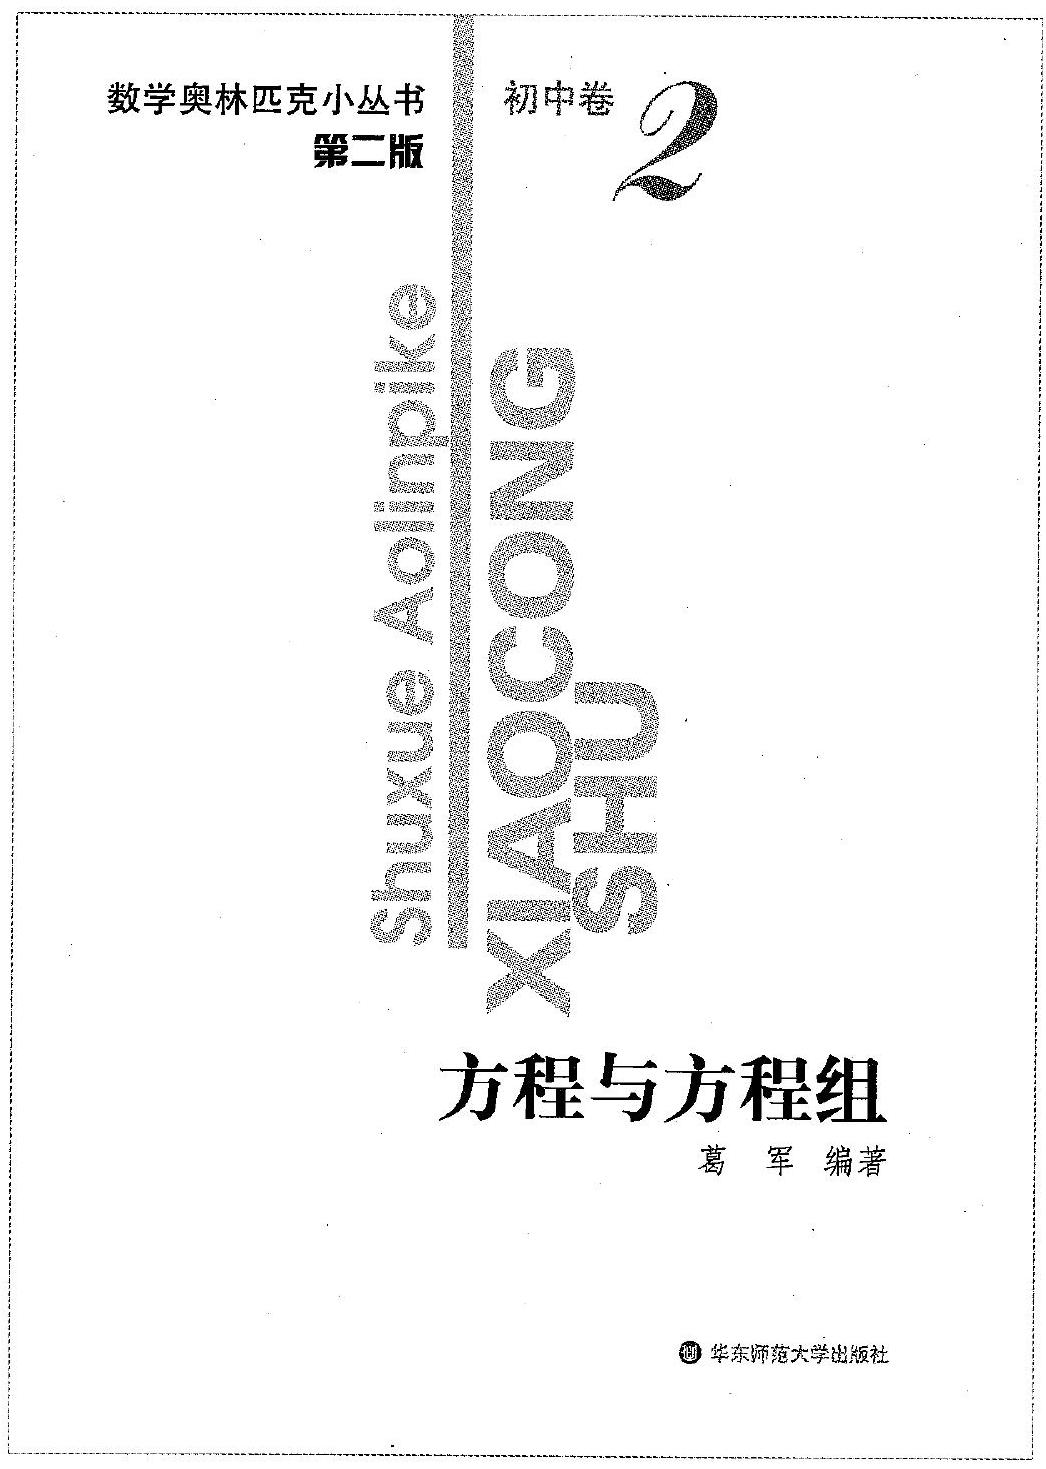
\includegraphics[max width=\textwidth, center]{2024_10_30_26b590fd1106d28139f0g-001}

物理竞赛群:271751860,化学竞赛群:271751511,生物竞赛群:254139830,信息竞赛群:281798334,英语竞赛群:271750414,英语 $\square$ 语群:168570356,心算交流群:131033273,厦门培训机构教师招聘

\section*{数学奥林匹克小丛书(第二版) 编委会}
冯志刚 第 53 届 $1 M O$ 中国队副领队、上海中学特级教师\\
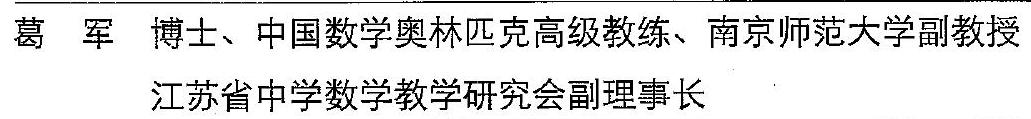
\includegraphics[max width=\textwidth, center]{2024_10_30_26b590fd1106d28139f0g-002}\\
冷岗松 国家集训队教练、上海大学教授、博士生导师

李胜宏 第44届1MO中国队领队、浙江大学教授、博士生导师\\
李伟固 中国数学奥林匹克委员会委员、国家集训队教练\\
北京大学教授、博士生导师\\
刘诗雄 华南师范大学中山附属中学校长、中学数学特级教师\\
倪 明 华东师范大学出版社教辅分社社长、编审\\
单 墫 第30、31届1MO中国队领队、南京师范大学教授、博士生导师\\
吴建平 中国数学会普及工作委员会主任、中国数学奥林匹克委员会副主席\\
熊 斌 第46、49、51、52、53届1MO中国队领队\\
中国数学奥林匹克委员会委员、华东师范大学教授、博士生导师\\
余红兵 中国数学奥林匹克委员会委员、国家集训队教练\\
苏州大学教授、博士生导师\\
朱华伟 中国教育数学学会常务副理事长、国家集训队教练\\
广州大学软件所所长、研究员

数学竞赛像其他竞赛活动一样,是青少年学生的一种智力竟赛。在类似的以基础科学为竞赛内容的智力竞赛活动中,数学竞赛的历史最悠久、国际性强,影响也最大。我国于1956年开始举行数学竞赛,当时最有威望的著名数学家华罗庚、苏步青、江泽涵等都积极参加领导和组织竞赛活动,并组织出版了一系列青少年数学读物,激励了一大批青年学生立志从事科学事业。我国于1986年起参加国际数学奥林匹克,多次获得团体总分第一,并于1990年在北京成功地举办了第 31 届国际数学奥林匹克,这标志着我国数学竞赛水平在国际上居领先地位,为各国科学家与教育家所瞩目。

我国数学竞赛活动表明,凡是开展好的地区和单位,都能大大激发学生的学习数学的兴趣,有利于培养创造性思维,提高学生的学习效率。这项竞赛活动,将健康的竞争机制引进数学教学过程中,有利于选拔人才。由数学竞赛选拔的优胜者,既有踏实广泛的数学基础,又有刻苦钻研、科学的学习方法,其中的不少青年学生将来会成为出色的科学工作者。在美国,数学竟赛的优胜者中后来成名如米尔诺(J. W. Milnor)、芒福德(D. B. Mumford)、奎伦 (D. Quillen)等都是菲尔兹数学奖的获得者;在波兰,著名数论专家辛哲尔 (A. Schinzel)学生时代是一位数学竞赛优胜者;在匈牙利,著名数学家费叶尔 (L. Fejér)、里斯(M. Riesz)、舍贵(G. Szegö)、哈尔(A. Haar)、拉多 (T. Radó)等都曾是数学竞赛获奖者。匈牙利是开展数学竞赛活动最早的国家,产生了同它的人口不成比例的许多大数学家!

在开展数学竞赛的活动同时,各学校能加强联系,彼此交流数学教学经验,从这种意义上来说,数学竟赛可能成为数学课程改革的"催化剂",成为培养优秀人才的有力措施。

不过,应当注意在数学竞赛活动中,注意普及与提高相结合,而且要以普及为主,使竞赛具有广泛的群众基础,否则难以持久。

当然,现在有些人过于关注数学竟赛的成绩,组织和参与都具有很强的功利目的,过分扩大数学竟赛的作用,这些都是不正确的,违背了开展数学竟赛活动的本意。这些缺点有其深层次的社会原因,需要逐步加以克服,不必因

为有某些缺点,就否定这项活动。\\
我十分高兴看到这套《数学奥林匹克小丛书》的正式出版。这套书,规模大、专题细。据我所知,这样的丛书还不多见。这套书不仅对数学竞赛中出现的常用方法作了阐述,而且对竞赛题作了精到的分析解答,不少出自作者自已的研究所得,是一套很好的数学竞赛专题教程,也是中小学生和教师的参考书。

这套小丛书的作者都是数学竞赛教学和研究人员,不少是国家集训队的教练和国家队的领队。他们为我国开展数学竞赛的活动和我国学生在 IMO上取得成绩、为国争光作出了贡献,为这套书尽早面世付出了艰辛的劳动。华东师大出版社在出版《奥数教程》和《走向 IMO》等竞赛图书基础上,策划组织了这套丛书,花了不少心血。我非常感谢作者们和编辑们在这方面所做的工作,并衰心祝愿我国的数学竞赛活动开展得越来越好。

\section*{五}
\footnotetext{王元,著名数学家,中国科学院院士,曾任中国数学会理事长、中国数学奥林匹克委员会主席.
}物理竞赛群:271751860,化学竞赛群:271751511,生物竞赛群:254139830,信息竞赛群:281798334,英语竞赛群:271750414,英语 语群:168570356,心算交流群:131033273,厦门培训机构教师招聘

\section*{夏门郑剑雄高中数学竞赛系列}
全国小学奥数群:221739457,全国初中奥数学生群:253736211,全国高中奥数学生群591782992全国初中奥数教练群112464128,全国高中奥数教练群195949359\\
竞赛公众号:新浪微博@郑剑雄 微信:v136257437 QQ:136257437\\
业务:初高中联赛班、培优班、美国高中数学、教师培训、机构教学产品研发、讲义资料出售等

\begin{enumerate}
  \item 看 $a$ 与 1 ..... 001\\
2 -元一次方程的求解 ..... 003\\
3 含字母系数的一次方程 ..... 008\\
4 -元一次方程的应用 ..... 013\\
5 二(多)元一次方程组 ..... 020\\
6 二(多)元一次方程组的应用 ..... 026\\
7 学会配方 ..... 035\\
8 认识一元二次方程 ..... 041\\
9 一元二次方程的判别式 ..... 049\\
10 根与系数的关系及其应用 ..... 055\\
11 高次方程 ..... 062\\
12 分式方程 ..... 068\\
13 无理方程 ..... 075\\
14 -元二烦方苼组 ..... 080\\
15 二(多) 元一次方程的整数镬 ..... 089\\
16 二元二次方程的整矮根 ..... 095\\
17 一元二次方程的应用 ..... 102\\
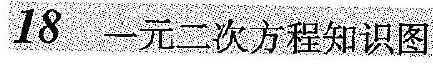
\includegraphics[max width=\textwidth]{2024_10_30_26b590fd1106d28139f0g-005} ..... 117习题解答119
\end{enumerate}

全国小学奥数群:221739457,全国初中奥数学生群:253736211,全国高中奥数学生群591782992全国初中奥数教练群112464128,全国高中奥数教练群195949359竞赛公众号:新浪微博@郑剑雄 微信:v136257437 QQ:136257437\\
业务:初高中联赛班、培优班、美国高中数学、教师培训、机构教学产品研发、讲义资料出售等

全国小学奥数群:221739457,全国初中奥数学生群:253736211,全国高中奥数学生群591782992全国初中奥数教练群112464128,全国高中奥数教练群195949359竞赛公众号:新浪微博@郑剑雄 微信:v136257437 QQ:136257437\\
业务:初高中联赛班、培优班、美国高中数学、教师培训、机构教学产品研发、讲义资料出售等

\section*{看 $a$ 与 1}
\begin{center}
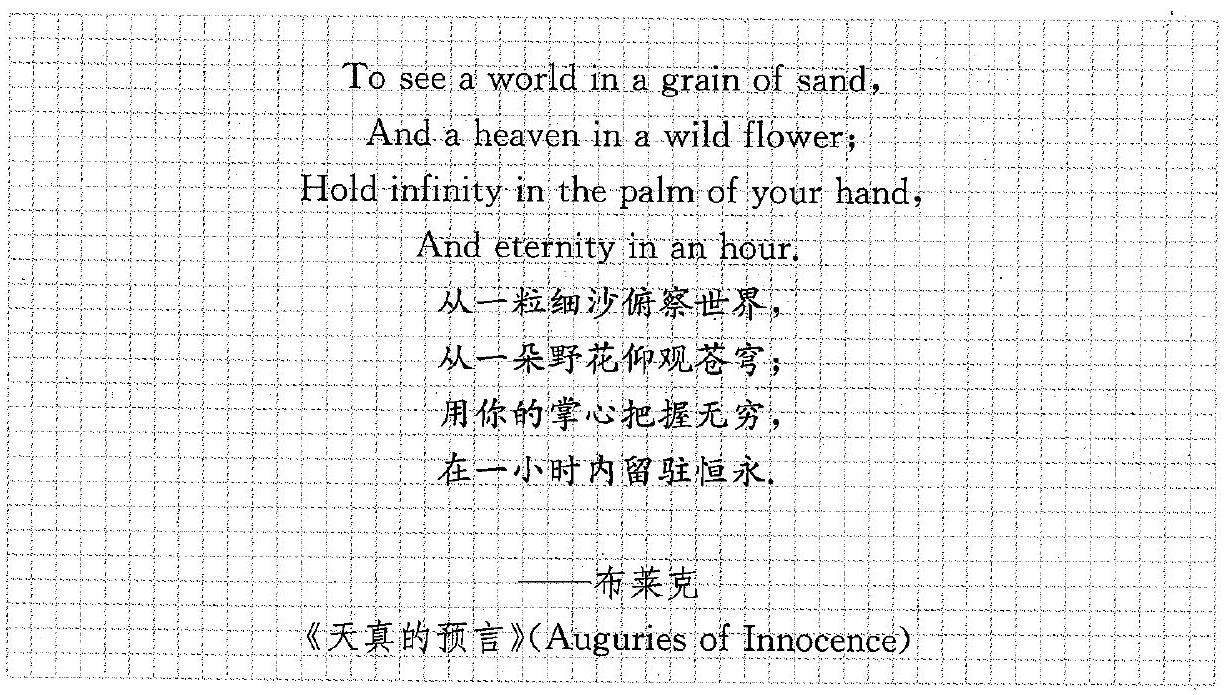
\includegraphics[max width=\textwidth]{2024_10_30_26b590fd1106d28139f0g-007}
\end{center}

大多数人总会认为如下的问题:\\
字母 $a$ 表示什么?\\
数字 1 是什么?\\
都是极为平凡的问题。\\
可是,你再仔细樵端详,用脑想一想,感觉不那么简单,而且想来很有趣,难道不是吗?!

字母 $a$ 表示什么呢? 转换你看问题的角度, 用 $a$ "丈量"你学习的足迹, 发现 $a$ 真的很丰富很生动。

你会说, $a$ 是 26 个英文字母表中排第一的字母; $a$ 可以代表正整数,可以代表分数,代表无理数、实数 $\cdots \cdots \cdot a$ 还可以代表一个算术算式,一个多项式如 $x-2, x^{2}+3 x-2$ ,代表分式如 $\frac{1}{x-3}$ ,代表无理式如 $\sqrt{x^{2}-2} \cdots \cdots a$ 还可以代表一个几何图形及其周长与面积……

你想 $a$ 是什么,它就是什么。

由此可以明白, $a$ 可表示单数"一",也包含着"all". 因此,你看 $a$ ,不能仅仅看成是一个"一",而是要看到"一切"。

其实,我们每个人都容易拥有一切,只需用你的眼光。但是,我们常常把自己框限于一个小小天地里,因此就会感觉到学得不够灵活,不够轻松。

让我们从现在开始,转换观念,由"一"想及"一切",则你必胜于"千里之外",不战而胜,且"胜于无形"之中。

说到数 1 ,与以上的认识一样,它也预示着"看我 1 ,不起眼,我却可以代表一切"。

读者在阅读这本小册子时,首先要做的,就是你的眼睛:"看 $a$ 不是 $a$ ", "看 1 不是 1 "。看" $a$ "应认为是你曾经的所有. 能做到吗?亲爱的读者们。\\
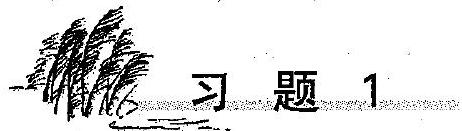
\includegraphics[max width=\textwidth, center]{2024_10_30_26b590fd1106d28139f0g-008}

试举几个具体例子,运用上述理念来进一步认识这些例子,并谈谈你自己的感受。

我思,故我在。\\
——笛卡儿

受过数学调练的人,应当比没有受过数学训练的人聪明一些,效率更高一些。\\
—单撙(摘自《解题研究》第22页,上海教育出版社,2007年4月)

让我们一起来玩列式游戏吧!\\
将数 2 和 3 、字母 $x$ ,用等号" $=$ "及四则运算符号"十、一、×、 $\div$ "中一个连接起来,可以得到哪些式子?

相信你可以写出很多个式子。\\
由前一讲" $a$ 与 1"的理解,你可以将它们归为四类,一类式子是形如 $x=$ $a \pm b, x=a \times b, x=a \div b$ ,这一类式子可以直接利用算术计算得 $x$ 的结果;第二类式子形如 $x+b=c$ ;第三类式子形如 $a x=c(a \neq 0)$ ;第四类式子形如 $\frac{a}{x}=c$ 。

对于式子 $x+b=c$ ,可以用加法与减法互为逆运算来计算,若一个数加上数 $b$ 等于数 $c$ ,则这个数等于 $c$ 减去 $b$ ,即 $x=c-b$ 。当我们用未知数 $x$ 来认识等式 $x+b=c$ 时,就称为一元一次方程 $x+b=c$ ,上述运算过程,又可以看作是将方程中的项 $b$ 从等号的左边移至右边且改变符号,使含未知数 $x$ 的项在等号的左边,已知数的式子在等号的右边。这个过程,在解方程中叫做移项,得 $x=c+(-b)$ ,即方程 $x+b=c$ 的解为 $x=c-b$ 。

对于 $a x=c$ ,在 $a \neq 0$ 的条件下,利用乘除互逆运算关系得 $x=c \times\left(\frac{1}{a}\right)$ ,即 $x=\frac{c}{a}$. 从方程的角度可以将上述过程看作是方程两边同除以 $a(a \neq 0)$ ,得 $x=\frac{c}{a}$, 即方程 $a x=c(a \neq 0)$ 的解为 $x=\frac{c}{a}$. 同样地, 对于第四类式子 $\frac{a}{x}=$ $c$, 先在两边同乘以 $x$, 得 $a=c x$, 化为第三类式子从而求得 $x=\frac{a}{c}$.

至此,我们会解方程 $a x=c(a \neq 0)$ 和 $x+b=c$ 了,如方程 $2 x=\frac{1}{3}$ 和 $x-3=1$ 的解就容易得到了,前者在方程两边同时除以 2 ,后者把 -3 移到等号右边,则这两个方程的解分别为 $x=\frac{1}{6}, x=4$ 。

再回首。多看一眼 $a x=c$ ,可以认识到 $a x+0=c$ ;多看一眼 $x+b=c$ ,可以认识到 $1 \cdot x+b=c$ 。据此,你自然想问若将" 0 " 换为数 $b$ ,将 " 1 "换为 $a$ 得到形如 $a x+b=c$ 的方程可以求解吗?

例如,方程 $3 x-5=4$ 如何求解呢?\\
必然地想到利用解形如方程 $a x=c, x+b=c$ 的基本解法。\\
首先,将一5改变符号后,移至等号右边,得

\begin{align*}
3 x=4+5 \text {, 即 } 3 x=9 \text {. }
\end{align*}

其次在方程 $3 x=9$ 的两边同时除以 3 ,得 $x=3$ 。\\
将 $x=3$ 代入原方程,验算知等式成立。(这一步在解多项式方程时可以略去,但在解分式方程时需将求得结果代回到原方程验算等式是否成立. 这一步骤又称为检验)。

所以,方程 $3 x-5=4$ 的解为 $x=3$ 。\\
因此,我们又会解方程 $a x+b=c(a \neq 0)$ 了。\\
尝试总结解方程 $a x+b=c$ 的步骤,并思考在解方程 $a x+b=c(a \neq 0)$时是否还可先两边同除 $a$ ,然后再移项呢?

例1 解方程 $\frac{1}{2} x+5=1$ 。\\
解法 1 移项得 $\frac{1}{2} x=1-5$, 即 $\frac{1}{2} x=-4$.\\
两边同除 $\frac{1}{2}$, 得 $x=(-4) \times 2$, 即 $x=-8$.\\
故原方程的解为 $x=-8$.\\
解法2 方程两边同除 $\frac{1}{2}$ ,得

\begin{align*}
\begin{gathered}
x+5 \times 2=1 \times 2, \text { 即 } x+10=2, \\
x=2-10, \text { 即 } x=-8 .
\end{gathered}
\end{align*}

移项得\\
故原方程的解为 $x=-8$ 。\\
说明 上述两个基本解法可根据实际选用。\\
例2 解方程 $3(x+2)-\frac{1}{3}(x-2)=4$ 。

基本思路 例 2 的方程与例 1 相比要复杂得多,因为它需要通过代数式的运算(合并同类项)将其转化为形如 $a x+b=c$ 或 $a x=c$ 的形式。因此首先要化简。

解 方程可化为

\begin{align*}
3 x+3 \times 2-\frac{1}{3} x+\frac{1}{3} \times 2=4
\end{align*}

合并同类项, 得 $\left(3-\frac{1}{3}\right) x+\left(3 \times 2+\frac{1}{3} \times 2\right)=4$,

即

\begin{align*}
\frac{8}{3} x+\frac{20}{3}=4,
\end{align*}

两边通分, 得 $8 x+20=4 \times 3$, 即 $8 x+20=12$.\\
移项得 $8 x=-8$ 。\\
两边同除 8 ,得 $x=-1$ 。\\
故原方程的解为 $x=-1$ 。\\
说明 通过解例 2 ,你能总结出解类似于例 2 的较为复杂的方程的步骤吗?

例3 小明在解方程 $3 a-2 x=15$ ( $x$ 为未知数)时,误将 $-2 x$ 看作是 $+2 x$ ,得方程的解为 $x=3$ ,试求出原方程的解。

基本思路 先按题设将方程改写为 $3 a+2 x=15$ ,然后利用方程的解的意义即 $x=3$ 使得等式成立,从而求得 $a$ 。最后解题设中的方程。

解 由题设知方程 $3 a+2 x=15$ 的解为 $x=3$ ,所以将 $x=3$ 代入方程得

\begin{align*}
3 a+2 \times 3=15 \text {, 即 } 3 a+6=15 \text {. }
\end{align*}

解这个关于 $a$ 的一元一次方程,得 $a=3$ 。\\
于是题中方程为 $9-2 x=15$ 。\\
解这个方程得 $\dot{x}=-3$ 。\\
故原方程的解为 $x=-3$ 。

\section*{例4 解方程}
\begin{align*}
\frac{3}{4}\left[\frac{4}{3}\left(\frac{1}{2} x-\frac{1}{4}\right)-8\right]=\frac{3}{2} x+1
\end{align*}

基本思路 别急,多读题。通常的做法是去括号,先去小括号再去中括号 $\cdots \cdots$ ,运算较繁。但是,你再读一遍,发觉可尝试先去中括号(因为 $\frac{3}{4} \times \frac{4}{3}=$

业务:初高中联赛班、培优班、美国高中数学、教师培训、机构教学产品研发、讲义资料出售等 1),可以简捷简化方程式。

解 题设方程可化为

得

\begin{align*}
\begin{gathered}
\left(\frac{1}{2} x-\frac{1}{4}\right)-6=\frac{3}{2} x+1 \\
\frac{1}{2} x-\frac{3}{2} x=1+\frac{1}{4}+6 \\
-x=7 \frac{1}{4} \\
x=-7 \frac{1}{4}
\end{gathered}
\end{align*}

故原方程的解为 $x=-7 \frac{1}{4}$.\\
说明(1)请读者尝试按通常做法解此方程,并指出按通常做法处理较为复杂方程时的优点之处。(2)解方程的过程不必拘泥于一定将含未知数的项移至方程式等号的左边。上述求解中,还可以将含未知数 $x$ 的项 $\frac{1}{2} x$ 移至等号右边,而数 1 移至左边,即 $-\frac{1}{4}-6-1=x$ 。

例 5 解方程 $|x+1|+3=5$ 。\\
基本思路 先移项 3 ,再用绝对值的意义分情况讨论,注意舍去不合题设的 $x$ (即增解)。

解 由 由方程 $|x+1|+3=5$ ,得

\begin{align*}
|x+1|=2
\end{align*}

当 $x+1 \geqslant 0$ 时, 有 $x \geqslant-1$, 且 $x+1=2$, 得 $x=1$.\\
当 $x+1<0$ 时, 有 $x<-1$ ,且 $x+1=-2$ ,得 $x=-3$ 。\\
将 $x=1$ 和 $x=-3$ 代人原方程,知 $x=1$ 和 $x=-3$ 均为原方程的解。\\
故原方程的解为 $x=-3, x=1$ 。\\
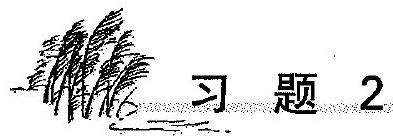
\includegraphics[max width=\textwidth, center]{2024_10_30_26b590fd1106d28139f0g-012}

解方程:(1) $0.5 x=19.5$ ;\\
(2) $\frac{x+3}{0.5}+\frac{\frac{1}{3}(x+4)}{0.125}=5 x+19$.

2 解方程:

业务:初高中联赛班、培优班、美国高中数学、教师培训、机构教学产品研发、讲义资料出售等\\
(1) $\frac{x+2}{4}-\frac{2 x-3}{6}=1$ ;\\
(2) $\frac{2 x+1}{3}-\frac{x-1}{2}=1$.

3 解方程:\\
(1) $3(2 x-3)-\frac{1}{3}(3-2 x)=7(3-2 x)-\frac{1}{7}(2 x-3)$;\\
(2) $x-\frac{1}{3}\left[x-\frac{1}{3}(x-9)\right]=\frac{1}{9}(x-9)$.

4 解方程:\\
(1) $2\left|x-\frac{1}{2}\right|-3=\frac{2}{3}$;\\
(2) $\frac{3}{4}\left\{\frac{4}{5}\left[\frac{2}{3}\left(\frac{1}{2} x-4\right)-2\right]+4\right\}-9=0$;\\
(3) $3\{2 x-1-[3(2 x-1)+3]\}=5$.

\section*{心智体操}
\section*{铅笔十橡皮 $=55$ 万美金}
律蒲曼是美国佛罗里达州的一位画家,他一度穷得除了画具和一支短短的铅笔之外一无所有。由于绘画时需要用橡皮擦,往往要花费很大功夫才能找到橡皮擦,待把画面擦好后又找不到铅笔了。如果把橡皮擦用丝线扎在铅笔的另一端上不就解决了吗?实验之下,他发现这种方法仅仅能够凑合使用,没多久,橡皮擦又从笔端掉落下来。

几经思考,他终于想出了一个好办法。他剪下一块薄铁皮片,把橡皮擦放在笔端,用铁皮片包起来,这样一来果然管用了。"说不定这玩意还能赚钱呢!"律蒲曼有了申请专利的念头。于是就找亲戚借钱申办了专利手续. 果不其然,当他将这项专利卖给 RABAR 铅笔公司时,他得到了 55 万美金。

全国小学奥数群:221739457,全国初中奥数学生群:253736211,全国高中奥数学生群591782992全国初中奥数教练群112464128,全国高中奥数教练群195949359竞赛公众号:新浪微博@郑剑雄 微信:v136257437 QQ:136257437\\
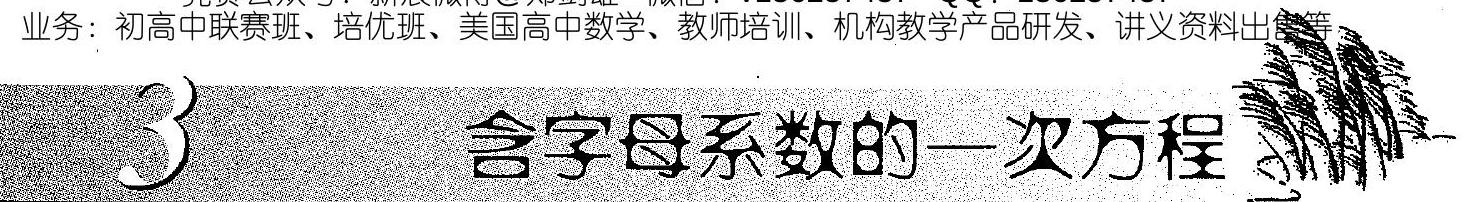
\includegraphics[max width=\textwidth, center]{2024_10_30_26b590fd1106d28139f0g-014(1)}\\
1.. it took men about five thousand years, counting from the beginning of number symbols, to think of a symbol for nothing.\\
….. 从产生数的符号算起,到想用一个符号来表示"无",足足花了人类约五千年的时间。

二阿西莫夫(摘自《阿西莫夫论数》)

适当地使用字母,可以使问题简化,规律变得明显。

\section*{与单墫(摘自《解题研究》第22页,上海教育出版社)}
在第 2 讲中,我们主要讨论了一元一次方程 $a x=b(a \neq 0)$ 的求解,这里 $a, b$ 是给定的数,知道了关于 $x$ 的方程在 $a \neq 0$ 的情形下方程的解为 $x=\frac{b}{a}$ 。

方程 $a x=b$ 又称为含字母系数的一元一次方程。\\
方程 $a x=b$ 对于 $a=0$ 和 $b=0$ ,可变形为 $0 \cdot x=0$ ,这表明 $x$ 有无数多个值满足此等式,即方程有无数多个解;对于 $a=0$ ,且 $b \neq 0$ ,方程变形为 $0 \cdot x$ $=b$ ,此等式不成立,这表明方程无解。

因此,方程 $a x=b$ 解的情形为: $a \neq 0$ 时方程有唯一解,为 $x=\frac{b}{a}, a=0$且 $b=0$ 时方程有无数多个解, $a=0$ 且 $b \neq 0$ 时方程无解。

利用上述结果可以方便地求解若干较为复杂的含字母系数的一元一次方程。\\
例1 解关于 $x$ 的方程: $4 a^{2}-x=2 a x+1$ 。\\
基本思路 移项转化为 $A x=B$ 的形式,利用平方差公式分解 $4 a^{2}-1$ ,然后讨论字母不同取值下方程的解的情况。

解 移项得

\begin{align*}
(2 a+1) x=4 a^{2}-1
\end{align*}

\begin{center}

\includegraphics[max width=\textwidth]{2024_10_30_26b590fd1106d28139f0g-014}
\end{center}

物理竞赛群:271751860,化学竞赛群:271751511,生物竞赛群:254139830,信息竞赛群:281798334,英语竞赛群:271750414,英语 语群:168570356,心算交流群:131033273,厦门培训机构教师招聘

利用 $4 a^{2}-1=(2 a-1)(2 a+1)$ ,方程又可变形为

\begin{align*}
(2 a+1) x=(2 a-1)(2 a+1)
\end{align*}

当 $2 a+1 \neq 0$ 时, $x=2 a-1$, 即当 $a \neq-\frac{1}{2}$ 时方程的解为 $x=2 a-1$;\\
当 $2 a+1=0$ 时, $0 x=0$, 即 $a=-\frac{1}{2}$ 时方程有无数多个解.\\
故 $a \neq-\frac{1}{2}$ 时,方程有唯一解,为 $x=2 a-1 ; a=-\frac{1}{2}$ 时,方程有无数多个解。

例2 解关于 $x$ 的方程 $m^{2}(1-x)=m x+1$.\\
基本思路 仿照例 1 变形方程。注意不要漏掉方程的解的讨论情况。\\
解 原方程变形为 $m^{2}-m^{2} x=m x+1$ 。\\
移项得

\begin{align*}
\begin{gathered}
\left(m^{2}+m\right) x=m^{2}-1 \\
m(m+1) x=(m-1)(m+1)
\end{gathered}
\end{align*}

当 $m \neq 0$ 且 $m \neq-1$ 时,方程的解为 $x=\frac{m-1}{m}$ ;\\
当 $m=0$ 时,原方程变为 $0 \cdot x=-1$ ,方程无解;\\
当 $m=-1$ 时,原方程变为 $0 \cdot x=0$ ,方程有无数多个解,其解为任意数。\\
故 $m \neq 0$ 且 $m \neq-1$ 时,方程有唯一解,为 $x=\frac{m-1}{m} ; m=0$ 时,方程无解; $m=-1$ 时,方程有无数多个解。

例3 19 个糖果盒排成一列,正中间的盒子放 $a$ 个糖果。从这里向右,每个盒子比前一个多 $m$ 个糖果;从这里向左,每个盒子依次比前一个多 $n$ 个糖果( $a, m, n$ 都是正整数)。如果糖果的总数是 1995 个,且 $a \geqslant 36$ 。求 $a$ 的值。

基本思路 按题设得到糖果总数为 $19 a+45 m+45 n$ ,然后利用因数分解及整除性,求得结果。

解 由题设得糖果总数为

\begin{align*}
\begin{aligned}
& a+(a+m)+(a+2 m)+\cdots+(a+9 m)+(a+n)+ \\
& (a+2 n)+\cdots+(a+9 n) \\
= & 19 a+\frac{m+9 m}{2} \times 9+\frac{n+9 n}{2} \times 9=19 a+45(m+n)
\end{aligned}
\end{align*}

又 $19 a+45(m+n)=1995$ ,则有

\begin{align*}
19 a=19 \times 105-45(m+n)
\end{align*}

业务:初高中联赛班、培优班、美国高中数学、教师培训、机构教学产品研发、讲义资料出售等

\begin{align*}
a=105-\frac{45 \times(m+n)}{19}
\end{align*}

因为 $a, m, n$ 均为正整数, 19 是质数, 所以 $m+n$ 一定是 19 的倍数, 但 $\frac{45 \times(m+n)}{19}$ 须小于 105 ,从而有

\begin{align*}
\begin{aligned}
& m+n=19, \text { 得 } a=60 ; \\
& m+n=19 \times 2, \text { 得 } a=15 .
\end{aligned}
\end{align*}

又题设中 $a \geqslant 36$ ,所以 $a$ 为 60 .

关于 $x$ 的方程 $a x=b$ ,逆向思考,我们可以有如下结论:\\
若方程有唯一解,则 $a \neq 0$ ;若方程有无数多个解,则 $a=0$ ,且 $b=0$ ;若方程无解,则 $a=0$ ,且 $b \neq 0$ 。

例4 若 $a b c=1$ ,解方程

\begin{align*}
\frac{2 a x}{a b+a+1}+\frac{2 b x}{b c+b+1}+\frac{2 c x}{c a+c+1}=1
\end{align*}

基本思路 注意到 $a b+a$ 中每项含有 $a$ ,则尝试将 1 代换为 $a b c$ ,这样可以简化式子 $\frac{2 a x}{a b+a+a b c}=\frac{2 x}{b+1+b c}$ ;同样地,将 $a b c$ 代换为 1 ,可变形式子 $\frac{2 c x}{c a+c+1}=\frac{2 b c x}{a b c+b c+b}=\frac{2 b c x}{b c+b+1}$ ,从而简化方程形式求得结果.

解 利用 $a b c=1$ ,可将原方程变形为

\begin{align*}
\begin{gathered}
\frac{2 a x}{a b+a+a b c}+\frac{2 b x}{b c+b+1}+\frac{2 b c x}{a b c+b c+b}=1 \\
\frac{2(1+b+b c) x}{b c+b+1}=1 \\
2 x=1 \\
x=\frac{1}{2}
\end{gathered}
\end{align*}

故方程的解为 $x=\frac{1}{2}$ 。\\
例 5 若一元一次方程 $a x=b$ 有两个不同的解 $x_{1}$ 和 $x_{2}$ ,求证:这个方程必有无数多个解。

证明 由题设 $x_{1}, x_{2}$ 都是方程 $a x=b$ 的解,得 $a x_{1}=b, a x_{2}=b$ 。于是

业务:初高中联赛班、培优班、美国高中数学、教师培训、机构教学产品研发、讲义资料出售等

即

\begin{align*}
a x_{1}=a x_{2}
\end{align*}

\begin{align*}
a\left(x_{1}-x_{2}\right)=0
\end{align*}

又因为 $x_{1} \neq x_{2}$, 所以必有 $a=0$. 从而

\begin{align*}
b=a x_{1}=0 \cdot x_{1}=0
\end{align*}

由于 $a=0$ 且 $b=0$ ,所以方程 $a x=b$ 有无数多个解。\\
说明 例 5 告诉我们,如果一个一元一次方程,只要有两个不同的解,那公它必有无数多个解。\\
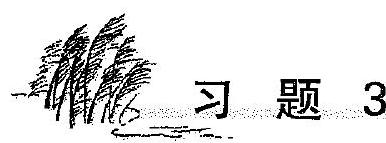
\includegraphics[max width=\textwidth, center]{2024_10_30_26b590fd1106d28139f0g-017}

\begin{itemize}
  \item 解关于 $x$ 的方程 $a x+1=b x$ 。
\end{itemize}

2 . 已知关于 $x$ 的方程 $3 m(x+3)=9 x+4$ 无解,求 $m$ 的值。\\
解关于 $x$ 的方程 $(a x-b)(a+b)=0$ 。\\
4 解关于 $x$ 的方程 $\frac{x}{a}+\frac{x}{b-a}=\frac{a}{a+b}\left(a \neq 0, a^{2} \neq b^{2}\right)$.\\
5 5设 $a$ 为整数,已知关于 $x$ 的方程 $|x|=a x+1$ 既有一个正根又有一个负根,求 $a$ 的值。

\section*{心智体操}
\section*{学会表述}
从前,有个人财大气粗,自命不凡,认为有钱能使鬼推磨,从没有办不成的事。但他肚子里缺少墨水,说起话来随随便便,从不考虑,就轻易出口。为此他得罪了很多人,朋友越来越少。有一天,他设宴请客,桌上摆满了鸡鸭鱼肉,山珍海味。来宾倒也不少。但他一看,却有几个重要的人物还没有到场,就不假思索,自言自语道:\\
"该来的怎么还不来呢?"\\
在座的客人们一听,心里凉了一大截,心想:照他这么说,我们是不该来的喽!于是有一半的人连招呼都不打就走了。

他一看,这么多人不辞而别,便着急地说:\\
"啊!不该走的都走了。"\\
剩下的人听了,心里好不生气,"他这么说,是当着和尚骂秃妭。这么说,

全国小学奥数群:221739457,全国初中奥数学生群:253736211,全国高中奥数学生群591782992全国初中奥数教练群112464128,全国高中奥数教练群195949359\\
竞赛公众号:新浪微博@郑剑雄 微信:v136257437 QQ:136257437\\
业务:初高中联赛班、培优班、美国高中数学、教师培训、机构教学产品研发、讲义资料出售等\\
我们是该走了!"于是,又有三分之二的人不告而别。\\
一看这阵势,这位东道主急得直拍大腿:\\
"这,这,我说的不是他们啊!"\\
剩下的三个客人听了,心里着实不是滋味,"不是说他们,那当然是说我们了。"于是,二话不说,也都气冲冲地打道回府了。

结果,宾客全都跑光了,只剩下主人一个人干着急。\\
你知道这位愣头愕脑的"马大哈"主人在说第一句话之前,已经到了多少客人吗?

如果没有数学的帮助和介入,对于大自然中的许多部分,我们既不能以足够的精细去阐明,也不能以足够的明晰去论证,还不能以足够的灵巧去应用。\\
——伽利略

现在,你已经会解一元一次方程了。你能否运用一元一次方程知识来处理一些实际问题呢?

事实上,我们是可以的。\\
因为处理实际问题时,我们只要多读题,善于用字母表示出实际问题中所涉及的对象和关系,并转化为一元一次方程,就变得易于解决了。有时,为了尽快地理解思路,需借助图表揭示实际问题中的关系,而迅捷地转化为一元一次方程。

从学习数学语言的角度看,处理实际问题就是需要我们学会玩语言的 "三角"转换,即实际文字语言、符号语言与图表语言之间的转化。让我们从现在起努力学会玩"语言三角"阦!

例1 某商店一种商品的进价降低了 $8 \%$ ,而售价保持不变,可使得商店的利润提高 $10 \%$ ,问:原来的利润率是百分之几?

基本思路 慢读,逐句理解清楚。回顾"进价",就是商店购进商品时的价格,可以大胆地尝试用字母表示,这里可以用 $a$ 表示原来的进价,"进价降低了 $8 \%$ "就是现在的进价为 $a \times(1-8 \%)$ 。"售价"就是实际销售的价格,"利润"是因销售商品而赚的钱,即利润三售价一进价,"利润率"就是利润与进价的百分比值。用 $\dot{x} \%$ 表示原来利润率,则原来的售价为"利润十进价" $=x \% \cdot a+a$ ,于是由"售价保持不变,可使商店的利润提高 $10 \%$ ",可得现在利润率为 $x \%+$ $10 \%$ ,从而有 $\frac{\text { 利润 }}{\text { 现进价 }} \times 100 \%=x \%+10 \%$ ,而"售价 - 现进价" $=(a+a \cdot$ $x \%)-a \times(1-8 \%)$ ,所以就得到式子: $a+a \cdot x \%-a \times(1-8 \%)=[a \times$\\
$(1-8 \%)] \cdot(x \%+10 \%)$ ,从而转化为含字母系数的一元一次方程了,求解此方程得结果。

解 设原来的进价为 $a$ 元,原利润率为 $x \%$ 。\\
由题设知原售价为 $(1+x \%) a$ 元,现在进价为( $1-8 \%) a$ 元,利润率为 $x \%+10 \%=(x+10) \%$ ,而现在的售价仍为 $(1+x \%) a$ ,所以现在利润 $=(1+$ $x \%) a-(1-8 \%) a$ 元,从而有

\begin{align*}
(1+x \%) a-(1-8 \%) a=(1-8 \%) a \cdot(x+10) \%
\end{align*}

可化为

\begin{align*}
(1+x \%)-(1-8 \%)=(1-8 \%)(x+10) \%
\end{align*}

\begin{align*}
\begin{gathered}
(100+x)-(100-8)=(100-8)(x+10) \times \frac{1}{100} \\
x+8=(x+10) \times \frac{92}{100}
\end{gathered}
\end{align*}

解得

\begin{align*}
x=15 .
\end{align*}

答:原来的利润率是 $15 \%$ 。\\
例2 "妇人洗碗在河滨,路人问她客几人?答曰不知客数目,六十五碗自分明,二人共食一碗饭,三人共吃一碗美,四人共肉无余数,请君细算客几人?"(摘自《孙子算经》)

基本思路 用 $x$ 表示客人数,"二人共食一碗饭"知饭碗用了 $\frac{x}{2}$ 只,"三人共吃一碗美"知美碗用了 $\frac{x}{3}$ 只,"四人共肉无余数"知肉碗用了 $\frac{x}{4}$ 只,共有碗 65只,则易于列出等式。

解 设客人有 $x$ 人,则饭碗用了 $\frac{x}{2}$ 只,美碗用了 $\frac{x}{3}$ 只,肉碗用了 $\frac{x}{4}$ 只.于是,根据题设得方程

\begin{align*}
\frac{x}{2}+\frac{x}{3}+\frac{x}{4}=65
\end{align*}

解得

\begin{align*}
x=60 . \tag{10}
\end{align*}

2\\
答:客人有 60 人.\\
9\\
3\\
例3 10 个人围成一个圆圈做游戏。游戏的规则是:每个人心里都想好一个数,并把自己想好的数如实地告诉他两旁的两个人,然后每个人将他两旁的两个人告诉他的数的平均数报出来。若报出来的数如图 4-1

5\\
6\\
图4-1

所示,则报 3 的人心里想的数是 $\qquad$。(2009 年全国初中数学竞赛题)\\
基本思路 设报 3 的人心里想的数是 $x$ ,报 5 的心里想的数是 $a$ ,那么报 4 的结果是 $a$ 与 $x$ 的平均数,即 $\frac{a+x}{2}=4$ ,得 $a=4 \times 2-x=8-x$ 。这样就可以知道报 5 的人心里想的数为 $8-x$. 同样的道理,报 7 的人心里想的数是 $6 \times 2-(8-x)=x+4$ ,报 9 的人心里想的数为 $8 \times 2-(x+4)=12-x$,报 1 的人心里想的数为 $2 \times 10-(12-x)=x+8$ ,报 3 的人心里想的数为 $2 \times 2-(x+8)=-x-4$ ,而这等于 $x$ ,得到方程。

解 设报 3 的人心里想的数是 $x$ ,则报 5 的人心里想的数应是 $4 \times 2$ -$x=8-x$ 。同理可知报 7 的人心里想的数是 $x+4$ ,报 9 的人心里想的数是 $12-$ $x$ ,报1的人心里想的数是 $x+8$ ,报 3 的人心里想的数是 $-4-x$ 。于是得

\begin{align*}
x=-4-x
\end{align*}

解得

\begin{align*}
x=-2
\end{align*}

例4 如图,一个高为 10 cm 、半径为 6 cm 的圆柱,以每分钟转一圈的速度旋转。一个宽为 3 cm 的刷子从圆柱侧面的顶端以每分钟移动 1 cm 的速度垂直向下移动。那么刷子刷过圆柱侧面 $50 \%$ 的面积所花的时间是 $\qquad$分钟。(2011 年"时代杯"江苏省中学数学应用与创新邀请赛题)\\
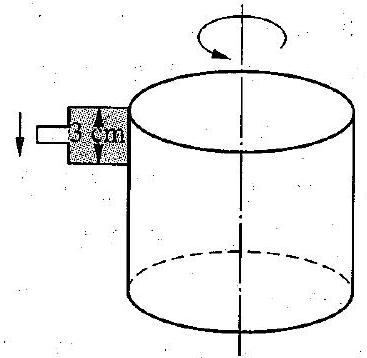
\includegraphics[max width=\textwidth, center]{2024_10_30_26b590fd1106d28139f0g-021}

图(1)\\
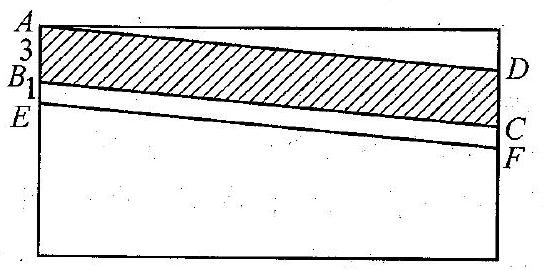
\includegraphics[max width=\textwidth, center]{2024_10_30_26b590fd1106d28139f0g-021(1)}

图(2)

图4-2\\
基本思路 刷子第一圈刷过的侧面展开图如图(2)。圆柱侧面展开图为矩形,图柱高 10 cm 为矩形的宽,长为 $2 \pi \times 6=12 \pi(\mathrm{~cm})$ 。第一圈刷子刷过侧.面展开图为平行四边形 $A B C D$ 。第 2 圈刷子垂直向下移动 1 cm ,得到一个小平行四边形带 $B C F E$ ,其面积为 $1 \times 2 \pi \times 6=12 \pi\left(\mathrm{~cm}^{2}\right)$ 。如此继续下去,每圈多刷出 $12 \pi \mathrm{~cm}^{2}$ 。这样,设经过 $t$ 分钟后刷子共刷过圆柱侧面的面积为 $3 \times 12 \pi+(t-$ 1) $\times 12 \pi$ ,当它是圆柱侧面的 $50 \%$ 时,就可以得到等式即方程。

解 设刷子经过 $t$ 分钟刷过圆柱侧面 $50 \%$ 的面积。

圆柱侧面积为 $2 \pi \times 6 \times 10=120 \pi\left(\mathrm{~cm}^{2}\right)$ ,圆柱侧面展开图中矩形的长为 $2 \pi \times 6=12 \pi(\mathrm{~cm})$ ,宽为 10 cm 。

由题设知第一圈刷过的面积为 $3 \times 12 \pi=36 \pi\left(\mathrm{~cm}^{2}\right)$, 从第 2 圈开始每圈多刷出 $1 \times 12 \pi=12 \pi\left(\mathrm{~cm}^{2}\right)$ 。于是有

\begin{align*}
36 \pi+12 \pi(t-1)=50 \% \times 120 \pi
\end{align*}

解得

\begin{align*}
t=3
\end{align*}

答:刷子刷过圆柱侧面 $50 \%$ 的面积所花的时间为 3 分钟。\\
说明 画一个草图如图(2)用以发现面积增加的规律。这是便捷解决实际问题的有益建议。

例 5 一辆客车、一辆货车和一辆小轿车在一条笔直的公路上朝同一方向匀速行驶。在某一时刻,客车在前,小轿车在后,货车在客车与小轿车的正中间。过了 10 分钟,小轿车追上了货车;又过了 5 分钟,小轿车追上了客车;再过 $t$ 分钟, 货车追上了客车, 则 $t=$ $\qquad$。(2010 年全国初中数学竞赛题)

基本思路 解这些较复杂的题,建议大胆用字母表示若干对象及其之间的数量关系,并借助于直观图理清它们之间的关系。读第一遍,知道了题的基本意思。读第二遍大胆设之,逐句列式,"在某一时刻,客车与货车,货车与小轿车之间的距离为 $S$ 千米,小轿车、货车、客车的速度分别为 $a, b, c$ 千米/分,货车经过 $x$ 分钟后追上客车。"过了 10 分钟,小轿车追上了货车"可以列式为 $10(a-b)=S$ ;"又过了 5 分钟,小轿车追上了客车",表明小轿车用 $10+5=15$ (分钟)追上了客车,即 $(10+5)(a-c)=2 S$ ;"货车经过 $x$ 分钟追上客车"即 $x(a-c)=S$ 。上述三个式子联立,消去 $a, b, c$ 后可以得到所求结果。

解 设在某一时刻,货车与客车、小轿车的距离均为 $S$ 千米,小轿车、货车、客车的速度分别为 $a, b, c$ 千米/分, 并设货车经过 $x$ 分钟追上客车, 则由题意得

\begin{align*}
\begin{aligned}
10(a-b) & =S \\
15(a-c) & =2 S \\
x(b-c) & =S
\end{aligned}
\end{align*}

由 $10(a-b)=S$ 及 $15(a-c)=2 S$ 得 $a-b=\frac{S}{10}, a-c=\frac{2 S}{15}$, 则

\begin{align*}
b-c=(b-a)+(a-c)=\frac{2 S}{15}-\frac{S}{10}=\frac{S}{30}
\end{align*}

\begin{center}

\includegraphics[max width=\textwidth]{2024_10_30_26b590fd1106d28139f0g-022}
\end{center}

物理竞赛群:271751860,化学竞赛群:271751511,生物竞赛群:254139830,信息竞赛群:281798334,英语竞赛群:271750414,英语 语群:168570356,心算交流群:131033273,厦门培训机构教师招聘

于是有

得

\begin{align*}
\begin{gathered}
\frac{S}{30} \cdot x=S \\
x=30
\end{gathered}
\end{align*}

所以

\begin{align*}
t=30-10-5=15 \text { (分). }
\end{align*}

例 6 一队旅客乘坐汽车,要求每辆汽车的乘客人数相等,起初,每辆汽车乘了 22 人,结果剩下一人未上车;如果有一辆汽车空车开走,那么所有旅客正好能平均分乘到其他各车上。 已知每辆汽车最多只能容纳 32 人,求起初有多少辆汽车?有多少名旅客?

基本思路 多读,大胆设元,转化为数学式子。设总人数为 $S$ ,起初有 $x$ 辆汽车,"起初每辆乘 22 人,结果剩下一人未上车",得 $22 x=S-1$ ;"开走一辆空车,乘客正好平均分到车上",得 $(x-1) k=S$ ,这里 $k$ 为正整数;又"每辆车最多只能容纳 32 人",即 $k \leqslant 32$ 。这样消去 $S$ ,并结合 $x, k$ 为正整数且 $k \leqslant 32$可得所求结果。

解 设起初有汽车 $x$ 辆,开走一辆空车后平均每辆车所乘的旅客为 $k$ 名。\\
由题意知 $22 x+1=k(x-1), x \geqslant 2, k \leqslant 32$ ,所以

\begin{align*}
k=\frac{22 x+1}{x-1}=22+\frac{23}{x-1}
\end{align*}

因为 $k$ 为正整数,所以 $\frac{23}{x-1}$ 为整数。而 23 为素数,那么 $x-1=1$ ,或 $x-$ $1=23$ ,得 $x=2$ ,或 $x=24$ 。

当 $x=2$ 时, $k=45$ 不合题意;\\
当 $x=24$ 时, $k=23$ 合题意,\\
这时旅客人数为 $k(x-1)=529$ 。\\
答:起初有 24 辆汽车,529名旅客。

\section*{习 题 4}
【I 已知一个多边形的内角和等于其外角和的 3 倍,求此多边形的边数。\\
2. $0 \sim 9$ 这 10 个数字每个恰用一次,组成若干个数,它们的和为 100 。问有多少种方法?\\
[3 甲、乙两个机器人同时从起点出发,沿跑道匀速向终点行进. 电子记录仪

表明:当甲距离终点 1 米时,乙距离终点 2 米;当甲到达终点时,乙距离终点 1.01 米。那么,跑道的长度为 $\qquad$米。\\
4 旅行者从下午 3 时步行到晚上 8 时,他先走平路,然后上山,到达山顶后就按原路下山,再走平路返回出发地。若他走平路每小时行 4 千米,上山每小时行 3 千米,下山每小时行 6 千米,问旅行者一共行多少千米?\\
5 如图为一个阶梯的纵截面,一只老鼠沿长方形的两边 $A \rightarrow B \rightarrow D$ 的路线逃跑,一只猫同时沿阶梯(折线) $A \rightarrow C \rightarrow D$ 的路线去捉,结果在距离点 $C 1.5$ 米的 $D$ 处,猫捉住了老鼠。已知老鼠的速度是猫的 $\frac{10}{13}$ ,问:阶梯 $A \rightarrow C$ 的长度是多少米?\\
66 游泳者在河中逆流而上,所带水壸于桥 $A$ 下被\\
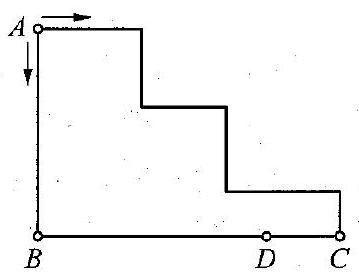
\includegraphics[max width=\textwidth, center]{2024_10_30_26b590fd1106d28139f0g-024}\\
(第 5 题)

水冲走。继续向前游了 20 分钟后他发现水亚遗失,于是立即返回,在桥 $A$ 下游距桥 $A 2$ 千米的桥 $B$ 下追到水壸。求该河水流的速度。\\
「梅林中学租用两辆小汽车(设速度相同)同时送 1 名带队老师及 7 名九年级的学生到县城参加数学竞赛,每辆限坐 4 人(不包括司机)。其中一辆小汽车在距离考场 15 km 的地方出现故障,此时离截止进考场的时刻还有 42 分钟,这时唯一可利用的交通工具是另一辆小汽车,且这辆车的平均速度是 $60 \mathrm{~km} / \mathrm{h}$ ,人步行的速度是 $5 \mathrm{~km} / \mathrm{h}$ (上、下车时间忽略不计)。\\
(1)若小汽车送 4 人到达考场,然后再回到出故障处接其他人,请你通过计算说明他们能否在截止进考场的时刻前到达考场;\\
(2)假如你是带队的老师,请你设计一种运送方案,使他们能在截止进考场的时刻前到达考场,并通过计算说明方案的可行性。

\section*{心智体操}
\section*{凸作"代换"}
从前有座山,山上有座庙,庙里有个老和尚和小和尚,老和尚喜欢算术,小和尚也很聪明。有一天,老和尚要求小和尚两天内把圆周率 $\pi$ 的值背到小数点后 20 位。小和尚看到师傅写给他的一串枯燥无味而又杂乱无序的数字,很是头疼。背了两天才能背出"3.1415 $926535 "$ ,再往后的数字就乱了。两天后,老和尚来检查时,小和尚没有能完成任务。老和尚罚他面壁思过,并再给他一天的时间,否则重罚。小和尚饥寒交迫地跪在佛像前,盯着这一串杂乱无序的

数字发呆,第三天的中午,小和尚看着师傅一个人在自由自在地喝酒,突然灵机一动,头脑中闪过一首诗,他在自己的头脑中理顺后,立刻跑到师傅的桌边说:"师傅,师傅,我背出来了。"老和尚道:"背来听听。"小和尚:"山顶一寺一壸酒,尔乐,苦杀吾,把酒吃,酒杀尔,杀不死,乐而乐"。老和尚大吃一惊,立即叫他与自己一起吃饭。此后逢人便夸小和尚聪明。小朋友,你知道为什么吗?

原来小和尚的那首诗正好与圆周率 $\pi$ 的值有关。\\
山顶一寺一壸酒,尔乐,苦杀吾,把酒吃,酒杀尔,杀不死,乐而乐。\\
$3.14159 \quad 26 \quad 535 \quad 897 \quad 932 \quad 384 \quad 626$

\section*{夏门郑剑雄高中数学竞赛系列}
全国小学奥数群:221739457,全国初中奥数学生群:253736211,全国高中奥数学生群591782992全国初中奥数教练群112464128,全国高中奥数教练群195949359\\
竞赛公众号:新浪微博@郑剑雄 微信:v136257437 QQ:136257437\\
业务:初高中联赛班、培优班、美国高中数学、教师培训、机构教学产品研发、讲义资料

落霞与弧燉齐飞,秋水共长天一色。

王勃(摘自《滕王图序》)

解二(多)元一次方程组的基本思想就是"消元",将二(多)元一次方程组转化为一元一次方程。恰似秋水共长天一色。常用的消元法有"加减消元法"和"代入消元法"。处理较为复杂的一次方程组时还需灵活运用等式的基本性质,以及"整体换元"等基本技巧。

例1 解方程组 $\left\{\begin{array}{l}x+3 y=-1, \\ 3 x-y=7 .\end{array}\right.$\\
基本思路 用代入消元法,将 $x=-1-3 y$ 代入另一方程 $3 x-y=7$ ,或将 $y=3 x-7$ 代入方程 $x+3 y=-1$ ;或用加减消元法,将方程式 $3 x-y=7$两边同乘以 3 后,与方程式 $x+3 y=-1$ 相加,消去 $y$ 元。

解法 1 由方程 $3 x-y=7$ 得 $y=3 x-7$ ,代入方程 $x+3 y=-1$ ,得

\begin{align*}
\begin{gathered}
x+3(3 x-7)=-1 \\
10 x=20
\end{gathered}
\end{align*}

解得 $x=2$, 代入方程 $y=3 x-7$ 得 $y=-1$.\\
故原方程组的解为 $\left\{\begin{array}{l}x=2, \\ y=-1 .\end{array}\right.$\\
解法 2 将方程 $3 x-y=7$ 两边同乘以 3 ,得

与方程\\
相加得\\
解得

\begin{align*}
9 x-3 y=7 \times 3
\end{align*}

\begin{align*}
x+3 y=-1
\end{align*}

\begin{align*}
9 x+x=21-1,
\end{align*}

\begin{align*}
x=2
\end{align*}

物理竞赛群:271751860,化学竞赛群:271751511,生物竞赛群:254139830,信息竞赛群:281798334,英语竞赛群:271750414,英语 $\square$ 语群:168570356,心算交流群:131033273,厦门培训机构教师招聘

将 $x=2$ 代入方程 $x+3 y=-1$, 得 $2+3 y=-1$, 解得 $y=-1$.\\
故方程组的解为 $\left\{\begin{array}{l}x=2, \\ y=-1 .\end{array}\right.$\\
说明 当方程组中有一个元的系数为 1 ,常用代人法使算术运算简便。当方程组中有一个元在两个方程中的系数或相等,或符号相反,常用加减消元法易于运算。

一般地,对于二元一次方程组

\begin{align*}
\left\{\begin{array}{l}
a_{1} x+b_{1} y=c_{1} \\
a_{2} x+b_{2} y=c_{2}
\end{array}\right.
\end{align*}

这里 $a_{1}, a_{2}, b_{1}, b_{2}$ 为已知数, $a_{1}$ 与 $b_{1}, a_{2}$ 与 $b_{2}$ 中都至少有一个不为零。\\
(1)当 $\frac{a_{1}}{a_{2}} \neq \frac{b_{1}}{b_{2}}$ 时,方程组有唯一一组解

\begin{align*}
\left\{\begin{array}{l}
x=\frac{b_{2} c_{1}-b_{1} c_{2}}{a_{1} b_{2}-a_{2} b_{1}} \\
y=\frac{a_{1} c_{2}-a_{2} c_{1}}{a_{1} b_{2}-a_{2} b_{1}}
\end{array}\right.
\end{align*}

(2)当 $\frac{a_{1}}{a_{2}}=\frac{b_{1}}{b_{2}}=\frac{c_{1}}{c_{2}}$ 时,方程组有无穷多组解;\\
(3)当 $\frac{a_{1}}{a_{2}}=\frac{b_{1}}{b_{2}} \neq \frac{c_{1}}{c_{2}}$ 时,方程组无解。\\
例 2 已知关于 $x$ 的方程 $2 a(3 x+2)-1=(2 b+1) x$ 有无数多个解,求 $a$ 与 $b$ 的值。

基本思路 由一元一次方程有无数多解的条件,列出二元一次方程组,解这个方程组,得结果。

解 由题设关于 $x$ 的方程可变形为

\begin{align*}
(6 a-2 b-1) x=1-4 a
\end{align*}

那么由此方程有无数多个解,得

\begin{align*}
\left\{\begin{array}{l}
6 a-2 b-1=0 \\
1-4 a=0
\end{array}\right.
\end{align*}

解得

\begin{align*}
a=\frac{1}{4}, b=\frac{1}{4}
\end{align*}

业务:初高中联赛班、培优班、美国高中数学、教师培训、机构教学产品研发、讲义资料出售等\\
故

\begin{align*}
a=\frac{1}{4}, b=\frac{1}{4} .
\end{align*}

例3 已知关于 $x, y$ 的方程组

\begin{align*}
\left\{\begin{array}{l}
a x+2 y=1+a  \tag{1}\\
2 x+2(a-1) y=3
\end{array}\right.
\end{align*}

分别求出当 $a$ 为何值时,方程组有唯一一组解;无解;有无穷多组解。\\
基本思路 用代入消元法。对于含字母的式子去乘或除方程的两边时,式子的值需不等于零。

解 由方程(1)得 $2 y=1+a-a x$ ,代人(2) 得

\begin{align*}
\begin{gather*}
2 x+(a-1)(1+a-a x)=3 \\
(a-2)(a+1) x=(a-2)(a+2)
\end{gather*} \tag{3}
\end{align*}

当 $(a-2)(a+1) \neq 0$ ,即 $a \neq 2$ 且 $a \neq-1$ 时,方程 (3) 有唯一解 $x=\frac{a+2}{a+1}$.代入 $2 y=1+a-a x$ ,得 $y=\frac{1}{2(a+1)}$ 。因此原方程组有唯一一组解。

当 $(a-2)(a+1)=0$ ,且 $(a-2)(a+2) \neq 0$ ,即 $a=-1$ 时,方程 (3) 无解。因此原方程组无解。

当 $(a-2)(a+1)=0$ ,且 $(a-2)(a+2)=0$ ,即 $a=2$ 时,方程 (3) 有无穷多个解。因此原方程组有无穷多组解。

例 4 设 $m, n$ 是给定的实数,已知关于 $x, y$ 的方程组 $\left\{\begin{array}{l}x+2 y=5, \\ m x-y=1+n\end{array}\right.$ 与 $\left\{\begin{array}{l}x-2 y=-3, \\ 2 n x+y=1+m\end{array}\right.$ 有相同的解, 求 $m, n$ 的值。(2011 年 "时代杯"江苏省中学数学应用与创新邀请赛题)

基本思路 先由方程的解的意义解方程组 $\left\{\begin{array}{l}x+2 y=5, \\ x-2 y=-3,\end{array}\right.$ 然后将所得解代人题设中的方程组,再解关于 $m, n$ 的方程组。

解 由题设解方程组 $\left\{\begin{array}{l}x+2 y=5, \\ x-2 y=-3,\end{array}\right.$ 得 $\left\{\begin{array}{l}x=1, \\ y=2 .\end{array}\right.$\\
将 $\left\{\begin{array}{l}x=1, \\ y=2\end{array}\right.$ 代入题设中的两个方程组, 得 $\left\{\begin{array}{l}m-2=1+n, \\ 2 n+2=1+m\end{array}\right.$\\
解之,得 $\left\{\begin{array}{l}m=5, \\ n=2 .\end{array}\right.$\\
例 5 求方程组 $\left\{\begin{array}{l}|x|+y=12, \\ x+|y|=6\end{array}\right.$ 的解的组数.(2007 全国初中数学竞赛

\section*{题改编)}
基本思路 根据绝对值的意义分情形转化为二元一次方程,要注意检验。\\
解 若 $x \geqslant 0$ ,则题设方程组转化为 $\left\{\begin{array}{l}x+y=12 , \\ x+|y|=6 ,\end{array}\right.$ 得 $|y|-y=-6$ ,而 $|y|-y \geqslant 0$, 所以不存在 $y$ 使得 $|y|-y=-6$ ,从而推知 $x \geqslant 0$ 时原方程组无解.

若 $x<0$, 则题设方程组转化为 $\left\{\begin{array}{l}-x+y=12, \\ x+|y|=6 .\end{array}\right.$\\
于是有 $|y|+y=18$, 解得 $y=9$, 从而求得 $x=-3$.\\
所以,原方程组的解为 $\left\{\begin{array}{l}x=-3 , \\ y=9 ,\end{array}\right.$ 只有 1 组解。\\
例 6 已知 $x, y, z$ 为实数,满足 $x+2 y-5 z=3, x-2 y-z=-5$ ,则 $x^{2}+y^{2}+z^{2}$ 的最小值为( ). (2011年全国初中数学竞赛题)\\
(A) $\frac{1}{11}$\\
(B) 0\\
(C) 5\\
(D) $\frac{54}{11}$

基本思路 将题设中等式看作是关于 $x, y$ 的二元一次方程组,解得 $x, y$关于 $z$ 的式子,然后代入 $x^{2}+y^{2}+z^{2}$ 中得到一个关于 $z$ 的一元二次式,则可利用完全平方公式 $(a+b)^{2}=a^{2}+2 a b+b^{2}$ 及完全平方值的非负性求得结果。

解 由 $\left\{\begin{array}{l}x+2 y-5 z=3, \\ x-2 y-z=-5,\end{array}\right.$ 可得 $\left\{\begin{array}{l}x=3 z-1, \\ y=z+2 .\end{array}\right.$\\
于是

\begin{align*}
\begin{aligned}
x^{2}+y^{2}+z^{2} & =11 z^{2}-2 z+5=11\left(z^{2}-2 \cdot z \cdot \frac{1}{11}+\frac{1}{121}\right)+5-\frac{1}{11} \\
& =11\left(z-\frac{1}{11}\right)^{2}+\frac{54}{11} \geqslant \frac{54}{11}
\end{aligned}
\end{align*}

因此,当 $z-\frac{1}{11}=0$ 即 $z=\frac{1}{11}$ 时, $x^{2}+y^{2}+z^{2}$ 最小,最小值为 $\frac{54}{11}$.\\
选 D.\\
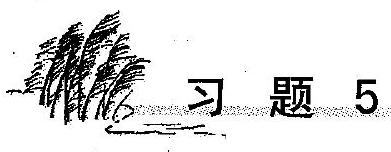
\includegraphics[max width=\textwidth, center]{2024_10_30_26b590fd1106d28139f0g-029}

【I 解方程组: (1) $\left\{\begin{array}{l}\frac{2 x-1}{5}+\frac{3 y-2}{4}=2, \\ \frac{3 x+1}{5}-\frac{3 y+2}{4}=0 .\end{array}\right.$\\
(2) $\left\{\begin{array}{l}\frac{x+y}{6}+\frac{x-y}{10}=3, \\ \frac{x+y}{6}-\frac{x-y}{10}=-1 .\end{array}\right.$

2 关于 $x, y$ 的两个方程组 $\left\{\begin{array}{l}a x-2 b y=2, \\ 2 x-y=7\end{array}\right.$ 和 $\left\{\begin{array}{l}3 a x-5 b y=9, \\ 3 x-y=11\end{array}\right.$ 具有相同的解,求 $a, b$ 的值.\\
5 已知关于 $x, y$ 的方程组 $\left\{\begin{array}{l}2 x+3 y=6, \\ a x+6 y=12 .\end{array}\right.$ 问 $a$ 为何值时, 方程组有无数多组解? $a$ 为何值时,只有一组解?\\
4. 对于任意的数 $a, b$ ,关于 $x, y$ 的二元一次方程 $(a-b) x-(a+b) y=a-$ $b$ 都有一组公共解,这组公共解为 $\qquad$。\\
5 甲 、乙两人解二元一次方程组

\begin{align*}
\left\{\begin{array}{l}
a x+5 y=13  \tag{1}\\
4 x-b y=-2
\end{array}\right.
\end{align*}

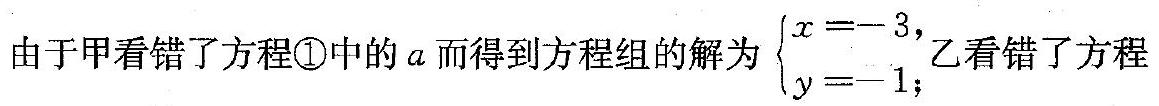
\includegraphics[max width=\textwidth]{2024_10_30_26b590fd1106d28139f0g-030(1)} (2) 中的 $b$ 而得到的解为 $\left\{\begin{array}{l}x=5, \\ y=4 .\end{array}\right.$ 求正确的 $a, b$ 值,并求出原方程组的解.

6 解方程组 $\left\{\begin{array}{l}\frac{x}{4}=\frac{y}{5}=\frac{z}{6}, \\ 2 x+3 y-4 z=-3 .\end{array}\right.$\\
7 解方程组 $\left\{\begin{array}{l}2 x+y+z=2, \\ x+2 y+z=4, \\ x+y+2 z=6 .\end{array}\right.$\\
8. 解方程组 $\left\{\begin{array}{l}|x-y|=x+y-2, \\ |x+y|=x+2 .\end{array}\right.$\\
9) 若 $x_{1}, x_{2}, x_{3}, x_{4}$ 和 $x_{5}$ 满足方程组

\begin{align*}
\left\{\begin{array}{l}
2 x_{1}+x_{2}+x_{3}+x_{4}+x_{5}=6 \\
x_{1}+2 x_{2}+x_{3}+x_{4}+x_{5}=12 \\
x_{1}+x_{2}+2 x_{3}+x_{4}+x_{5}=24 \\
x_{1}+x_{2}+x_{3}+2 x_{4}+x_{5}=48 \\
x_{1}+x_{2}+x_{3}+x_{4}+2 x_{5}=96
\end{array}\right.
\end{align*}

试确定 $3 x_{4}+2 x_{5}$ 的值.\\

\includegraphics[max width=\textwidth, center]{2024_10_30_26b590fd1106d28139f0g-030}

物理竞赛群:271751860,化学竞赛群:271751511,生物竞赛群:254139830,信息竞赛群:281798334,英语竞赛群:271750414,英语 $\square$ 语群:168570356,心算交流群:131033273,厦门培训机构教师招聘\\
10. 已知 $\frac{a+b}{a-b}=\frac{b+c}{2(b-c)}=\frac{c+a}{3(c-a)}, a, b, c$ 互不相等. 求证:

\begin{align*}
8 a+9 b+5 c=0
\end{align*}

\section*{心智体操}
解题是一种实践性的技能,就像游泳、滑雪或弹钢琴一样,只能通过模仿和实践学到它……你想学会游泳,你就必须下水,你想成为解题高手,你就必须去解题。\\
——波利亚\\
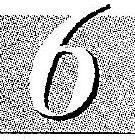
\includegraphics[max width=\textwidth, center]{2024_10_30_26b590fd1106d28139f0g-032}

\section*{二 (多)元一次方程组的应用}
宇宙之大,粒子之微,火箭之速,化工之巧,地球之变,生物之谜,日月之繁,无处不用数学。

应用二(多)元一次方程组来解决实际问题时,首要的依然是多读题,善于用字母将题中对象及关系表示出来,进而利用等式基本性质简化所求问题的代数式(即二(多)元一次方程组),求得实际问题的结果。

例1 鸡兔共 100 只,鸡的脚比兔的脚多 80 只,问鸡与兔各多少只?(摘自《孙子算经》)

基本思路 利用鸡的只数与其脚数、兔的只数与其脚数之间的关系,列出方程组。

解 设鸡有 $x$ 只,兔有 $y$ 只,则由题意知

解得

\begin{align*}
\begin{gathered}
\left\{\begin{array}{l}
x+y=100 \\
2 x-4 y=80
\end{array}\right. \\
\left\{\begin{array}{l}
x=80 \\
y=20
\end{array}\right.
\end{gathered}
\end{align*}

所以,鸡有 80 只,兔有 20 只。\\
说明 上述问题是鸡兔同笼问题,在小学里运用假设法及算术知识处理了与本题类似的问题。但是其处理的方式较之代数的解法(设未知数,列出方程组)来说较难(同学们可以再体会一下)。代数的方法具有统一性,各种各样的问题可以用同样的方法处理,而且复杂的应用题,特别是涉及多个对象及关系多重的应用题,往往只能用代数方法来处理。

例2 小王沿街匀速行走,发现每隔 6 分钟从背后驶过一辆 18 路公交车,每隔 3 分钟从迎面驶来一辆 18 路公交车。假设每辆18路公交车行驶速度

相同,而且 18 路公交车总站每隔固定时间发一辆车,那么发车间隔的时间是\\
$\qquad$分钟。(2008 年全国初中数学竞赛题)\\
基本思路 大胆用字母表示,令同向行驶的相邻两车的间距为 $s$ 米,18路公交车和小王行走的速度分别 $x 、 y$ 米 / 分。利用题设条件列出方程组。

解 设 18 路公交车的速度是 $x$ 米/分,小王行走的速度是 $y$ 米/分,同向行驶的相邻两车的间距为 $s$ 米。

每隔 6 分钟从背后开过一辆 18 路公交车,则

\begin{align*}
6 x-6 y=s \tag{1}
\end{align*}

每隔 3 分钟从迎面驶来一辆 18 路公交车,则

\begin{align*}
3 x+3 y=s \tag{2}
\end{align*}

由(1),(2)可得 $s=4 x$ ,所以 $\frac{s}{x}=4$ 。\\
答:18路公交车总站发车间隔的时间是4分钟。\\
例3 有四个正整数,其中任三个数的算术平均数与第四个数的和,分别等于 $29,23,21,17$ ,则这四个数中最大的一个是 $\qquad$。\\
基本思路 分别令四个数为 $x, y, z, w$, 列出四元一次方程组,解这个方程组。

解 设四个数分别为 $x, y, z, w$ ,则由题设知

\begin{align*}
\left\{\begin{array}{l}
\frac{1}{3}(x+y+z)+w=29 \\
\frac{1}{3}(x+y+w)+z=23 \\
\frac{1}{3}(x+z+w)+y \Rightarrow 21 \\
\frac{1}{3}(y+z+w)+x=17
\end{array}\right.
\end{align*}

上述四个方程相加得

\begin{align*}
2(x+y+z+w)=90, x+y+z+w=45
\end{align*}

因为

\begin{align*}
\begin{aligned}
& \frac{1}{3}(x+y+z)+w=\frac{1}{3}(x+y+z+w)+\frac{2}{3} w \\
& \frac{1}{3}(x+y+w)+z=\frac{1}{3}(x+y+z+w)+\frac{2}{3} z \\
& \frac{1}{3}(x+z+w)+y=\frac{1}{3}(x+y+z+w)+\frac{2}{3} y
\end{aligned}
\end{align*}

\begin{align*}
6 \text { 二(多)元一次方程组的 }
\end{align*}

应用

物理竞赛群:271751860,化学竞赛群:271751511,生物竞赛群:254139830,信息竞赛群:281798334,英语竞赛群:271750414,英语口语群:168570356,心算交流群:131033273,厦门培训机构教师招聘

业务:初高中联赛班、培优班、美国高中数学、教师培训、机构教学产品研发、讲义资料出售等

\begin{align*}
\frac{1}{3}(y+z+w)+x=\frac{1}{3}(x+y+z+w)+\frac{2}{3} x
\end{align*}

所以由 $29>23>21>17$ 知道 $\frac{2}{3} w>\frac{2}{3} z>\frac{2}{3} y>\frac{2 x}{3}$, 得 $w>z>$ $y>x$ ,即 $w$ 是最大数. 于是,由

\begin{align*}
\left\{\begin{array}{l}
x+y+z+w=45, \\
\frac{1}{3}(x+y+z+w)+\frac{2}{3} w=29,
\end{array}\right.
\end{align*}

得 $\frac{2}{3} w+\frac{1}{3} \times 45=29$ ,解得 $w=21$ 。\\
所以,这四个数中最大的一个是 21 。\\
说明 在上述解答过程中,可以直接由 $x+y+z+w=45$ 及上述方程组中的每个方程分别求解出 $z=12, y=9, x=3$ ,从而知 $w$ 为最大数。

例4 某纸品加工厂制作了甲、乙两种无盖的长方体小盒,如图 6-1,然后又利用边角料裁出了正方形硬纸片 150 张,长方形硬纸片 300 张,并且长方形的宽与正方形边长相等,如图 6-2. 再将这些硬纸片全部用于制作这种小盒,还可做成甲、乙两种小盒各多少个?\\
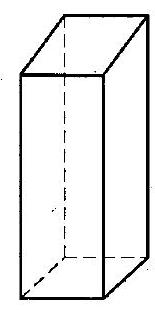
\includegraphics[max width=\textwidth, center]{2024_10_30_26b590fd1106d28139f0g-034(1)}

甲\\
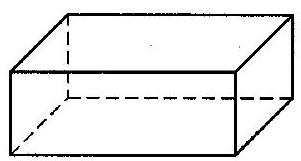
\includegraphics[max width=\textwidth, center]{2024_10_30_26b590fd1106d28139f0g-034(4)}

乙\\
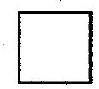
\includegraphics[max width=\textwidth, center]{2024_10_30_26b590fd1106d28139f0g-034}

图6-1\\
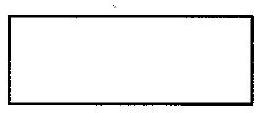
\includegraphics[max width=\textwidth, center]{2024_10_30_26b590fd1106d28139f0g-034(2)}

图 6-2

基本思路 甲种小盒每个由 1 张正方形纸片和 4 张长方形纸片组成,乙种小盒每个由 2 张正方形纸片和 3 张长方形纸片组成,因此,可令甲、乙两种小盒的个数分别为 $x, y$ ,那么甲种小盒共需要 $x$ 张正方形纸片及 $4 x$ 张长方形纸片,乙种小盒共需要 $2 y$ 张正方形纸片及 $3 y$ 张长方形纸片,从而得到 $x$ , $y$ 的方程组。

解 设可做成甲、乙两种小盒各 $x$ 个, $y$ 个,则 $x$ 个甲种小盒需要 $x$ 张正方形纸片和 $4 x$ 张长方形纸片, $y$ 个乙种小盒需要 $2 y$ 张正方形纸片和 $3 y$ 张长方形纸片。于是,由题设得\\

\includegraphics[max width=\textwidth, center]{2024_10_30_26b590fd1106d28139f0g-034(3)}

\begin{align*}
\left\{\begin{array}{l}
x+2 y=150 \\
4 x+3 y=300
\end{array}\right.
\end{align*}

解得

\begin{align*}
\left\{\begin{array}{l}
x=30 \\
y=60
\end{array}\right.
\end{align*}

答:可做成甲、乙两种小盒各 30 个、 60 个.\\
例5 $A, B, C$ 三人各有糖若干粒,要求互相赠送。先由 $A$ 给 $B, C$ ,所给的糖数等于 $B, C$ 原来各有的糖数,依同法再由 $B$ 给 $A, C$ 现有糖数,后由 $C$给 $A, B$ 现有糖数,互送后每人恰好各有 64 粒。问原来三人各有糖多少粒?

基本思路 题中条件较为复杂,列出一个表来揭示相互间的等量关系,这是一个转化实际问题的基本方式。在大胆设元 $A 、 B 、 C$ 三人各有糖 $x 、 y 、 z$粒之下,仔细列表正确表示出变化过程中的量的关系。

解 设 $A, B, C$ 三人原来各有 $x, y, z$ 粒糖,依题意可列出下表:

\begin{center}
\begin{tabular}{|c|c|c|c|}
\hline
 & $A$ & $B$ & $C$ \\
\hline
原有 & $x$ & $y$ & $z$ \\
\hline
\begin{tabular}{l}
第一次 \\
赠送后 \\
\end{tabular} & $x-y-z$ & $2 y$ & $2 z$ \\
\hline
\begin{tabular}{l}
第二次 \\
赠送后 \\
\end{tabular} & $2(x-y-z)$ & $2 y-(x-y-z)-2 z$ & $4 z$ \\
\hline
\begin{tabular}{c}
第三次 \\
赠送后 \\
\end{tabular} & $4(x-y-z)$ & $4 y-2(x-y-z)-4 z$ & \begin{tabular}{c}
$4 z-2(x-y-z)-2 y+$ \\
$(x-y-z)+2 z$ \\
\end{tabular} \\
\hline
\end{tabular}
\end{center}

由此可得

\begin{align*}
\left\{\begin{array}{l}
4(x-y-z)=64 \\
4 y-2(x-y-z)-4 z=64 \\
4 z-2(x-y-z)-2 y+(x-y-z)+2 z=64
\end{array}\right.
\end{align*}

解得

\begin{align*}
\left\{\begin{array}{l}
x=104 \\
y=56 \\
z=32
\end{array}\right.
\end{align*}

答:原来甲有糖 104 粒,乙有糖 56 粒,丙有糖 32 粒。\\
说明 在解决实际问题时,需常想到列表或画一个示意图。这是可以简捷得到解题思路的良好方式。

例6 一个时钟有时针与分针但钟面上并没有数字。在早上 $T$ 时刻,钟在

\begin{align*}
\begin{gathered}
6 \text { 二 (多) 元一次方程组的 } \\
\text { 应用 }
\end{gathered}
\end{align*}

镜子中的影像显现出早上 $X$ 时刻,且 $X$ 比 $T$ 迟了 5 小时 28 分,问 $T$ 是早上几时几分。

基本思路 首先知道在时钟上每小时时针移动 $30^{\circ}$ ,将两个时刻的时间关系转化为圆上圆心角之间的关系,列出关于两个时刻时针所对应角度 $\alpha, \beta$的方程组,解出 $\alpha, \beta$ 之后,再对应到时刻 $T$ 与 $X$ 。

解 由题设,两个时刻 $X$ 与 $T$ 之差为 5 小时 28 分,设(从 12 点处出发顺时针方向计算) $X$ 时刻时针对应的角度为 $\alpha, T$ 时刻时针对应的角度为 $\beta$ ,则在钟面上它们所对应的角度之差是

\begin{align*}
\alpha-\beta=\left(5 \frac{28}{60}\right) \times 30^{\circ}=164^{\circ}
\end{align*}

又因为它们之间的角度关系是 $\alpha+\beta=360^{\circ}$ ,所以有方程组 $\left\{\begin{array}{l}\alpha-\beta=164^{\circ} \\ \alpha+\beta=360^{\circ},\end{array}\right.$ 解得 $\beta=\frac{360^{\circ}-164^{\circ}}{2}=$ $98^{\circ}, \frac{98}{30}=3 \frac{4}{15}$ ,所以对应的 $T$ 时刻为 3 时 16 分.

答: $T$ 是早上 3 时 16 分。\\
例7 一个十位数字为 0 的三位数,它恰好等于它的数字和的 67 倍;交换它的个位与百位数字后\\
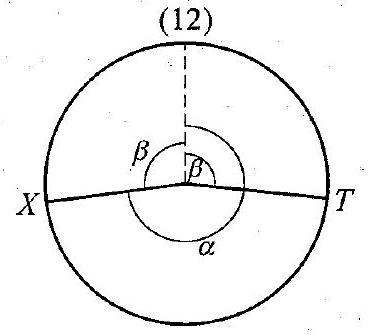
\includegraphics[max width=\textwidth, center]{2024_10_30_26b590fd1106d28139f0g-036}

图6-3

得到一个新的三位数,它恰好又是数字和的 $m$ 倍,求 $m$ 的值。

基本思路 利用十进位制知识可设百位、个位上数字分别是 $x 、 y$ ,得出关于 $x, y$ 的方程组,整体析出 $x+y$ ,从而直接求得 $m$ 。

解 设原三位数的百位数字为 $x$ ,个位数字为 $y$ ,由题意得

\begin{align*}
\left\{\begin{array}{l}
100 x+y=67(x+y) \\
100 y+x=m(x+y)
\end{array}\right.
\end{align*}

上述两个方程相加得

\begin{align*}
101 \cdot(x+y)=(67+m)(x+y) .
\end{align*}

由 $x+y>0$ 得

\begin{align*}
\begin{gathered}
67+m=101 \\
m=34
\end{gathered}
\end{align*}

答: $m$ 的值为 34 。\\
例8 有一片牧场,草每天都匀速地生长(草每天增长的量相等)。若在牧场上放牧 24 头牛,则 6 天吃完牧草;若放牧 21 头牛,则 8 天吃完牧草。设每头牛每天吃草的量都是相等的。问:(1)如果放牧 16 头牛,那么几天可以吃完牧草?\\
(2)要使牧草永远吃不完,至多放牧几头牛?

基本思路 本题是熟知的"牛吃草问题"。需考虑草每天的增长量 $y$ ,每头牛每天的吃草量 $x$ ,牧场原有的草量 $a$ 和 16 头牛 $z$ 天吃草量或 $w$ 头牛吃草量之间的关系,逐步列出方程组。

解 (1)设每头牛每天吃草量为 $x$ ,草每天增长量为 $y$ ,牧场原有的草量为 $a, 16$ 头牛 $z$ 天可以吃完牧草。

根据题意得 $x>0, y>0, z>0$ ,且

\begin{align*}
\left\{\begin{array}{l}
a+6 y=24 \times 6 x  \tag{1}\\
a+8 y=21 \times 8 x \\
a+y z=16 x z
\end{array}\right.
\end{align*}

(2) -(1)得

\begin{align*}
y=12 x \tag{3}
\end{align*}

(3) - (2)得

\begin{align*}
(z-8) y=8 x(2 z-21) \tag{4}
\end{align*}

将(4)代人(5)得

\begin{align*}
(z-8) \times 12 x=8 x(2 z-21) \tag{5}
\end{align*}

\begin{align*}
3(z-8)=2(2 z-21)
\end{align*}

解得

\begin{align*}
z=18
\end{align*}

(2)设放牧 $w$ 头牛, 牧草永远吃不完, 则必须使 $w$ 头牛每天吃的草量不大于草每天的增长量,即

\begin{align*}
x \cdot w \leqslant y . \tag{6}
\end{align*}

(4)代入(6)得

由 $x>0$ 知

\begin{align*}
x w \leqslant 12 x .
\end{align*}

\begin{align*}
w \leqslant 12
\end{align*}

所以至多放牧 12 头牛。\\
答:若放牧 16 头牛,则 18 天可以吃完牧草;要使牧草永远吃不完,至多放牧 12 头牛。

说明 "问什么,设什么",这是解决实际问题的基本要求,不是表述转化实际问题为代数问题的唯一目的要求,若这样,复杂问题中量与量关系就难以直接明白快捷地转化为数学问题了。因此,用较多字母表示出题中量与量之间关系,是处理实际问题的良好意识,需要学习者极力注重培养。

例 9 现有含糖 $15 \%$ 的糖水 20 克,含糖 $40 \%$ 的糖水 15 克,另有足够多的糖和水,要配制成含糖 $20 \%$ 的糖水 30 克。\\
(1)试设计多种配制方案;\\
(2)试对你的各种配制方案作一评价,哪一种用糖最省?哪一种现有糖水的浪费最少?\\
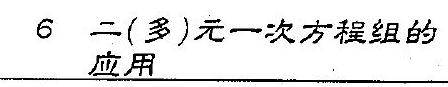
\includegraphics[max width=\textwidth, center]{2024_10_30_26b590fd1106d28139f0g-037}

基本思路 溶液的配制方案可以是:只用糖与水;不用含糖 $40 \%$ 的糖水;不用含糖 $15 \%$ 的糖水;两种糖水各用 10 克等。分别列出上面四种方案所对应的二元一次方程组,然后解方程组,并比较相应的量的大小。

解(1)因为有两种不同含糖量的糖水和足够多的糖和水供配制之用,于是可以有下面四种方案(还可有其他方案):\\
(1) 不用现有的糖水,只用糖和水。

设用糖 $x$ 克,用水 $y$ 克,则

\begin{align*}
\left\{\begin{array} { l } 
{ x + y = 3 0 , } \\
{ x = 3 0 \times 2 0 \% , }
\end{array} \text { 解得 } \left\{\begin{array}{l}
x=6, \\
y=24 .
\end{array}\right.\right.
\end{align*}

(2) 将含糖 $15 \%$ 的糖水 20 克全用上,但不用含糖 $40 \%$ 的糖水。

设用糖 $x$ 克,用水 $y$ 克,则

\begin{align*}
\left\{\begin{array} { l } 
{ 2 0 + x + y = 3 0 , } \\
{ 2 0 \times 1 5 \% + x = 3 0 \times 2 0 \% }
\end{array} \text { 解得 } \left\{\begin{array}{l}
x=3, \\
y=7 .
\end{array}\right.\right.
\end{align*}

(3) 将含糖 $40 \%$ 的糖水 15 克全用上,但不用含糖 $15 \%$ 的糖水。

由于含糖 $40 \%$ 的糖水 15 克中有糖 6 克,而所要配制的含糖 $20 \%$ 的糖水 30 克也有糖 6 克,数量相等,所以只要用含糖 $40 \%$ 的糖水 15 克再加水 15 克即可。\\
(4) 用两种糖水各 10 克。

设用糖 $x$ 克,用水 $y$ 克,则

\begin{align*}
\left\{\begin{array} { l } 
{ 1 0 + 1 0 + x + y = 3 0 , } \\
{ 1 0 \times 1 5 \% + 1 0 \times 4 0 \% + x = 3 0 \times 2 0 \% , }
\end{array} \text { 解得 } \left\{\begin{array}{l}
x=0.5, \\
y=9.5 .
\end{array}\right.\right.
\end{align*}

(2)上述各种解法中,第(3)种方法用糖最省(不用糖)。\\
第(2)、(4)种方法与其他方法比较,现有糖水用得最多(浪费最少),有没有比现有糖水浪费更少的方法?理想的方法是 30 克糖水均由现有糖水构成,即不加糖和水。

设用含量 $15 \%$ 的糖水 $x$ 克,含糖 $40 \%$ 的糖水 $y$ 克,则

\begin{align*}
\left\{\begin{array} { l } 
{ x + y = 3 0 , } \\
{ x \times 1 5 \% + y \times 4 0 \% = 3 0 \times 2 0 \% , }
\end{array} \text { 解得 } \left\{\begin{array}{l}
x=24, \\
y=6 .
\end{array}\right.\right.
\end{align*}

但含糖 $15 \%$ 的糖水总共才有 20 克( $<24$ 克),故此解答不切实际,由于缺少的 4 克 $15 \%$ 的糖水中的糖分可用 $40 \%$ 的糖水补充,所以最省的方法应是只加水,不加糖。

设用现有糖水共 $y$ 克,其中含糖 $15 \%$ 的糖水 $x$ 克,加水 $a$ 克,则

\begin{align*}
\left\{\begin{array}{l}
x \times 15 \%+(y-x) \times 40 \%=30 \times 20 \% \\
y+a=30
\end{array}\right.
\end{align*}

整理得 $y=\frac{5}{8} x+15(0 \leqslant x \leqslant 20)$, 当 $x=20$ 时, $y_{\text {樶大 }}=27.5$, 此时 $a=30-y=2.5$

即用 $15 \%$ 的糖水 20 克, $40 \%$ 的糖水 7.5 克,加水 2.5 克,可使现有糖水浪费最少。\\
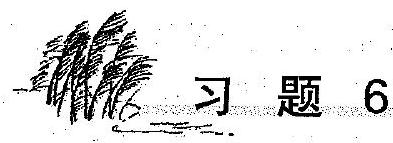
\includegraphics[max width=\textwidth, center]{2024_10_30_26b590fd1106d28139f0g-039}

1 有若干只鸡和兔子同笓,它们共有 88 个头, 244 只脚,问鸡和兔各有多少只?\\
2-项世博工程,由甲乙两个工程队合作 7 个月可以完成,现两队合作 5 个月后,甲队所有队员及乙队人数的 $\frac{1}{5}$ 调整做其他工作,又过了 6 个月由剩下的人把工程完成. 如果甲乙单独做,那么甲需要几个月,乙需要几个月?\\
3. 汽车以每小时 72 千米的速度在公路上行驶,开向寂静的山谷,驾驶员按一声喇叭,4秒后听到回响,这时汽车离山谷多远?(声音的速度以 340米/秒计算)\\
4有两种铁矿石,甲铁矿石含铁 $68 \%$ ,乙铁矿石含铁 $63 \%$ ,现要配制含铁 $65 \%$ 的混合铁矿石 100 吨,两种铁矿石应各取多少吨?\\
5 小强问叔叔有多少岁,叔叔说:"我像你这么大时,你才 4 岁;你到我这么大时,我就 40 岁了。"问小强和叔叔今年各是多少岁?\\
6 一批货物准备运往某地,有甲、乙、丙三辆卡车可以租用。已知甲、乙、丙三辆车每次运货量一定,如果甲、乙两车单独运这批货物,则甲车运送的次数是乙车运送次数的 2 倍;如果同时租用甲、丙两车,用相同次数运完这批货物时,甲车运了 180 吨;如果同时租用乙、丙两车,用相同次数运完这批货物时,乙车运了 270 吨。如果同时租用甲、乙、丙三车,用相同次数把这批货物运完,货主应付这三辆车车主运费各多少元(每运 1 吨付运费 20 元)?\\
■ 一个自行车轮胎,若把它安装在前轮,则自行车行驶 5000 km 后报废;若把它安装在后轮,则自行车行驶 3000 km 后报废,行驶一定路程后可以交换前、后轮胎。如果交换前、后轮胎,要使一辆自行车的一对新轮胎同时报废,那么这辆车将能行驶多少千米。(2009 全国初中数学竞赛题)\\
8要有五只猴子平均分一堆桃子,不能恰好分完。天黑了,它们把桃子留在原\\
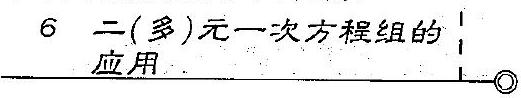
\includegraphics[max width=\textwidth, center]{2024_10_30_26b590fd1106d28139f0g-039(1)}

地,各自找一块地方睡觉去。月亮出来了,其中的一只猴子偷偷地跑过来,扔掉多余的一个桃子,剩下的桃子正好可以平均分成五份,它抱起自己应得的一份,回去睡觉了。过了一会儿,另一只猴子跑过来,也扔掉一个桃子,剩下的桃子刚好能平均分成五份,它也抱走自己的一份回去了。\\
(1)问原来的那一堆桃子至少应该是多少个?\\
(2) 若第三、第四、第五只猴子, 它们来了以后也是和前面两个猴子一样,扔掉一个,然后拿走自己的一份. 问原来的桃子至少有多少个?最后至少剩下多少个桃子?\\
-9一旅游团 50 人到一旅舍住宿,旅舍的客房有三人间、二人间、单人间三种,其中三人间的每人每晚 20 元,二人间的每人每晚 30 元,单人间的每晚 50 元.\\
(1)若旅游团共住满了 20 间客房,问三种客房各住了几间?怎样住消费最低?\\
(2)该旅游团中,若安排是夫妻的住二人间, 单身的(成人)住三人间,小孩可随父母住在一起。现已知有 4 对夫妻各带了 1 个小孩,单身的 30人,其中男性 17 人,有 2 名单身神经衰弱患者要求住单人间,问这一行人共需多少间客房?

\section*{心智体操}
\begin{enumerate}
  \item 托尔斯泰的分数:
\end{enumerate}

俄国大文豪托尔斯泰在谈到对人的评价时,把人比作一个分数。他说: "一个人就好像一个分数,他的实际才能好比分子,而他对自己的估价好比分母. 分母越大,则分数值就越小。"\\
2. 比尼:贝笛,你知道吗?

什么东西有两个脑袋、六条腿、一根尾巴?\\
贝笛:一个人骑在马背上。\\

\includegraphics[max width=\textwidth, center]{2024_10_30_26b590fd1106d28139f0g-040}

物理竞赛群:271751860,化学竞赛群:271751511,生物竞赛群:254139830,信息竞赛群:281798334,英语竞赛群: 271750414, 英语 语群: 168570356, 心算交流群: 131033273 , 夏门培训机构教师招聘

\section*{一切的一,光明呀!}
一的一切,光明呀!\\
光明便是你,光明便是我!\\
光明便是"他",光明便是火!\\
—郭沫若《成凰湦䑁》一一風》更生歌

在小学里,我们就学过"一个数加 2 等于 6 ,求这个数"这样的问题,如果用方程表示就是

\begin{align*}
x+2=6 \tag{1}
\end{align*}

这里的 $x$ 表示所求的数。解这个方程,对大家来说,是一件轻松而又容易的事,在(1)中移项就可以得到

\begin{align*}
x=4
\end{align*}

但是,如果是"一个数的平方加 2 ,等于 6 ,求这个数",那么又如何求呢?同样地,我们可以设所求的数为 $x$ ,则有

\begin{align*}
x^{2}+2=6, \tag{2}
\end{align*}

即

\begin{align*}
x^{2}=4
\end{align*}

我们知道,2的平方等于 $4,-2$ 的平方也等于 4 ,所以 $x=2$ 或 $x=-2$ 。\\
因此,对于 $x^{2}=4$ ,用根式表示就是 $x= \pm \sqrt{4}$ ,即 $x= \pm 2$ 。\\
一般地,对于 $x^{2}=a(a \geqslant 0)$ ,就有 $x= \pm \sqrt{a}$ 。\\
让我们换个角度来认识(1)与(2)的关系,我们发现(2)式可以看作是(1)式中 $x^{\prime}$ 生长"为 $x^{2}$ 得到的,即

\begin{align*}
x \rightarrow x^{2}
\end{align*}

现在,对" $x^{2}$ "中的 $x$ 来玩"生长",那么,我们能得到什么样的结果呢?看着 $x^{2}=4$ ,想着 $x$ 生长为 $x-3$ ,这个等式又变成怎样的形式呢?

我们用流程图表示就是

即

\begin{align*}
\begin{align*}
& x^{2}=4 \\
& \downarrow \text { 用 }(x-3) \text { 替换 } x \\
& (x-3)^{2}=4 \\
& \downarrow \text { 完全平方式展开 } \\
& x^{2}-6 x+9=4 \\
& \text { 移项、合并同类项 } \\
& x^{2}-6 x+5=0 .
\end{align*} \tag{3}
\end{align*}

得\\
这个(3)式即方程 $x^{2}-6 x+5=0$ 将如何求解呢?\\
回头看刚才的"生长过程",认识"来而不往非理也"。\\
我们发现:可以先利用完全平方公式配成平方,然后用根式的定义 $\left(x^{2}=\right.$ $a$ ,得 $x= \pm \sqrt{a}$ )求得方程的解,也就是:

得

即

得

即

\begin{align*}
x^{2}-6 x+5=0,
\end{align*}

\begin{align*}
\left(x^{2}-2 \times 3 x+3^{2}\right)+5-3^{2}=0
\end{align*}

\begin{align*}
\begin{gathered}
(x-3)^{2}=4, \\
x-3=2 \text { 或 } x-3=-2, \\
x=5 \text { 或 } x=1 .
\end{gathered}
\end{align*}

上述求解方程的关键就是"配方"。\\
运用前面所说的观念,学会看数 $6 、 5$ 不仅是数,它们可以变成字母 $b 、 c$ ,即看" $x^{2}-6 x+5=0$ "是" $x^{2}+b x+c=0$ "。那么,解这个方程 $x^{2}+b x+$ $c=0$ 的关键就是配方。

如何熟练地对二次三项式进行配方呢?关键在于熟练地运用 $a^{2}+2 a b+$ $b^{2}=(a+b)^{2}$ ,即看到 $a^{2}+b^{2}$ 想到找 $2 a b$ ,或者看到 $a^{2}+2 a b$ 想到找 $b^{2}$ 。

试举几例,期望读者拥有良好的配方感觉。\\
例1 分解因式: $\left(a^{2}-1\right)\left(b^{2}-1\right)+4 a b$ 。\\
基本思路 先展开试试,即 $\left(a^{2}-1\right)\left(b^{2}-1\right)=a^{2} b^{2}-a^{2}-b^{2}+1$ ,得

\begin{align*}
a^{2} b^{2}-\left(a^{2}+b^{2}\right)+1+4 a b
\end{align*}

试着:看 $a^{2} b^{2}+1$ 找 $2 a b$ ,看 $a^{2}+b^{2}$ 也找 $2 a b$ ,是否就可以分解了。\\
解 $\left(a^{2}-1\right)\left(b^{2}-1\right)+4 a b$

\begin{align*}
\begin{aligned}
& =a^{2} b^{2}-\left(a^{2}+b^{2}\right)+1+4 a b \\
& =a^{2} b^{2}+2 a b+1-\left(a^{2}+b^{2}-2 a b\right) \\
& =(a b+1)^{2}-(a-b)^{2} \\
& =(a b+1+a-b)(a b+1-a+b)
\end{aligned}
\end{align*}

思考 尝试看 $a^{2} b^{2}+4 a b$ 想到找 4 ,你能顺利地分解因式吗?你得到怎样的体会?

例2 已知 $a, b$ 都是大于 1 的正整数,求证: $a^{4}+4 b^{4}$ 是合数。\\
基本思路 看 $4 b^{4}=\left(2 b^{2}\right)^{2}, a^{4}=\left(a^{2}\right)^{2}$ ,想到 $2 \cdot a^{2} \cdot\left(2 b^{2}\right)\left(=4 a^{2} b^{2}\right)$ 。尝试配方,并用平方差公式因式分解。

解 由 $a^{4}+4 b^{4}$ 想到 $4 a^{2} b^{2}$ ,则有

\begin{align*}
\begin{aligned}
a^{4}+4 b^{4} & =a^{4}+4 a^{2} b^{2}+4 b^{4}-4 a^{2} b^{2} \\
& =\left(a^{2}+2 b^{2}\right)^{2}-(2 a b)^{2} \\
& =\left(a^{2}+2 b^{2}-2 a b\right)\left(a^{2}+2 b^{2}+2 a b\right) \\
& =\left[(a-b)^{2}+b^{2}\right]\left[(a+b)^{2}+b^{2}\right]
\end{aligned}
\end{align*}

由于 $a>1, b>1$, 所以 $(a-b)^{2}+b^{2}>1,(a+b)^{2}+b^{2}>1$.\\
因而 $a^{4}+4 b^{4}$ 是合数。\\
此题虽然做完了,但不要轻易放在一边,留足时间,再回首,品其韵味。\\
其一,问自己,什么样的整数 $a$ 与 $b$ ,使得 $a^{4}+4 b^{4}$ 是质数(除 1 及自身外无其他约数)?

其二,问自己, $a^{4}+4 b^{4}$ 可以写成四个数的平方和吗?如果能,这四个数可以不同吗?

例3 在实数范围内解方程

\begin{align*}
\sqrt{x}+\sqrt{y-1}+\sqrt{z-2}=\frac{1}{2}(x+y+z)
\end{align*}

基本思路 乍一看,怎生了得,从未见过。但冷静一想,三个未知数一个方程,必有倥门;再仔细一瞧, $x$ 与 $\sqrt{x}, y-1$ 与 $\sqrt{y-1}, z-2$ 与 $\sqrt{z-2}$ 之间的关系,想到配方。试试看!

解 原式整理为 $x+y+z-2 \sqrt{x}-2 \sqrt{y-1}-2 \sqrt{z-2}=0$,看 $x-2 \sqrt{x},(y-1)-2 \sqrt{y-1},(z-2)-2 \sqrt{z-2}$ 得

\begin{align*}
(x-2 \sqrt{x}+1)+[(y-1)-2 \sqrt{y-1}+1]+
\end{align*}

业务:初高中联赛班、培优班、美国高中数学、教师培训、机构教学产品研发、讲义资料出售等

\begin{align*}
[(z-2)-2 \sqrt{z-2}+1]=0
\end{align*}

即

\begin{align*}
(\sqrt{x}-1)^{2}+(\sqrt{y-1}-1)^{2}+(\sqrt{z-2}-1)^{2}=0
\end{align*}

由平方数是非负的,得

\begin{align*}
\begin{gathered}
\sqrt{x}-1=0, \sqrt{y-1}-1=0, \sqrt{z-2}-1=0 \\
x=1, y=2, z=3
\end{gathered}
\end{align*}

即\\
思考 你能运用第 1 讲中的"观念",得到类似于例 3 的问题,并努力尝试解决它们吗?

例4 说明 $n^{2}+n+1$ ( $n$ 是正整数)不是完全平方数。\\
基本思路 按题意,考虑 $n^{2}+n+1$ 介于两个连续数的平方之间,努力寻找这样的两个平方数。

解 由于 $n^{2}<n^{2}+n+1<n^{2}+2 n+1=(n+1)^{2}$, 所以 $n^{2}+n+1$ 不是完全平方数。

思考(1)试判别 $n^{2}+n+1$ ( $n$ 是整数)是否一定不是完全平方数?\\
(2)你会解决" $n^{2}+r(1 \leqslant r \leqslant 2 n, n, r$ 是正整数)不是完全平方数"的问题吗?

例 5 已知一个四边形的四条边长分别为 $a, b, c, d$ ,它们满足等式

\begin{align*}
a^{4}+b^{4}+c^{4}+d^{4}=4 a b c d
\end{align*}

试判断这个四边形的形状。\\
解 努力得到一些完全平方式,看到 $a^{4}+b^{4}$ 想到 $-2 a^{2} b^{2}$ ,看到 $c^{4}+d^{4}$ 想到 $-2 c^{2} d^{2}$ 。

\begin{align*}
\begin{aligned}
& a^{4}+b^{4}+c^{4}+d^{4}-4 a b c d \\
= & \left(a^{4}+b^{4}-2 a^{2} b^{2}\right)+\left(c^{4}+d^{4}-2 c^{2} d^{2}\right)+ \\
& 2 a^{2} b^{2}+2 c^{2} d^{2}-4 a b c d
\end{aligned}
\end{align*}

恰好有 $a^{2} b^{2}+2 a b c d+c^{2} d^{2}$ 是完全平方式,所以由

\begin{align*}
a^{4}+b^{4}+c^{4}+d^{4}-4 a b c d=0
\end{align*}

得

\begin{align*}
\left(a^{4}-2 a^{2} b^{2}+b^{4}\right)+\left(c^{4}-2 c^{2} d^{2}+d^{4}\right)+2\left(a^{2} b^{2}-2 a b c d+c^{2} d^{2}\right)=0
\end{align*}

即

\begin{align*}
\left(a^{2}-b^{2}\right)^{2}+\left(c^{2}-d^{2}\right)^{2}+2(a b-c d)^{2}=0
\end{align*}

得

\begin{align*}
a^{2}-b^{2}=0, c^{2}-d^{2}=0, a b-c d=0
\end{align*}

\begin{center}

\includegraphics[max width=\textwidth]{2024_10_30_26b590fd1106d28139f0g-044}
\end{center}

物理竞赛群:271751860,化学竞赛群:271751511,生物竞赛群:254139830,信息竞赛群:281798334,英语竞赛群:271750414,英语口语群:168570356,心算交流群:131033273,厦门培训机构教师招聘

由于 $a, b, c, d$ 都是正数,所以 $a=b=c=d$ 。\\
因此,这个四边形是菱形。\\
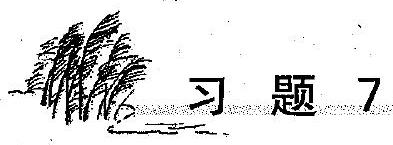
\includegraphics[max width=\textwidth, center]{2024_10_30_26b590fd1106d28139f0g-045}

1 已知 $x^{2}+y^{2}+4 x-6 y+13=0$, 其中 $x, y$ 均是实数,求 $x+2 y$ 的值.\\
2. 已知 $a, b, c$ 为三角形的三边长, 且满足

\begin{align*}
a^{2}+b^{2}+c^{2}+338=10 a+24 b+26 c
\end{align*}

试判断这个三角形的形状。\\
3 试确定方程 $\left(a^{2}+1\right) x^{2}-2 a x+\left(a^{2}+4\right)=0$ 的实根的个数。\\
4 实数 $a, b$ 满足关系 $a^{2} b^{2}+a^{2}+b^{2}+1=4 a b$ ,试求 $a+b$ 的值。\\
5 已知 $a, b, c, x, y, z$ 都是非零实数,且

\begin{align*}
a^{2}+b^{2}+c^{2}=x^{2}+y^{2}+z^{2}=a x+b y+c z
\end{align*}

求证: $\frac{x}{a}=\frac{y}{b}=\frac{z}{c}$ 。\\
6. 已知 $a, b, c$ 是三角形 $A B C$ 的三边长, 且满足

\begin{align*}
\frac{2 a^{2}}{1+a^{2}}=b, \frac{2 b^{2}}{1+b^{2}}=c, \frac{2 c^{2}}{1+c^{2}}=a,
\end{align*}

试求三角形 $A B C$ 的面积。\\
-7 设多项式 $a x^{2}+b x+c$ 为 $s$ ,若对任意实数 $x, s$ 满足

\begin{align*}
x^{2}+2 x+2 \leqslant s \leqslant 2 x^{2}+4 x+3,
\end{align*}

且 $x=9$ 时, $s=121$, 求 $a+b+c$ 的值. (2011 年全国初中数学竞赛题改编)

\section*{心智体操}
\section*{只需要 10 分神}
\section*{一个故事:}
有一个小男孩每天坚持练钢琴 4 个小时。他的老师知道后对他说:"你不能这样练,马上停止。因为你长大以后根本没有这么多的时间来练琴,你应该养成一有空闲就练的习惯,即使几分钟也行。"男孩听从了老师的劝告,把练钢琴的时间分解到各个时间段。其他时间用来写日记、培植标本、到草地上

业务:初高中联赛班、培优班、美国高中数学、教师培训、机构教学产品研发、讲义资料出售等踢足球,而这一切,并没影响他的琴艺。

这个小男孩后来成为著名的诗人、小说家和极其出色的钢琴家,他之所以在各个领域取得辉煌的成就,原因在于他能分解自己的爱好到每天的时间中,他即使只有 5 分钟的空闲也会利用起来,或写几句诗,或弹一首曲子。

几分钟的时间并不长,但如果能利用它并能成为一种习惯,这些短短的时间就有可能成就一个人,因为再大的事业和成就所需要的数年和数十年的时间都是由短短的几分钟累加起来的。当然这些应该是毫不拖延并加以充分利用的几分钟。

\section*{夏门郑剑雄高中数学竞赛系列}
全国小学奥数群:221739457,全国初中奥数学生群:253736211,全国高中奥数学生群591782992全国初中奥数教练群112464128,全国高中奥数教练群195949359\\
竞赛公众号:新浪微博@郑剑雄 微信:v136257437 QQ:136257437\\
业务:初高中联赛班、培优班、美国高中数学、教师培训、机构教学产品研发、讲义资料出售等\\

\includegraphics[max width=\textwidth, center]{2024_10_30_26b590fd1106d28139f0g-047}

横看成岭侧成峰,\\
远近高低各不同。\\
不现庐山真面目,只缘身在此山中。\\
——苏转《题西林壁》

在第 7 讲中,我们已经认识了一元二次方程 $x^{2}+b x+c=0$ ,自然地,我们也认识了(看二次项系数 1 ,非" 1 "是 $a$ )一元二次方程的一般形式

\begin{align*}
a x^{2}+b x+c=0
\end{align*}

不仅如此,想必你也知道如何求这个方程的解了。\\
那就是配方!\\
因为

\begin{align*}
\begin{aligned}
a x^{2}+b x+c & =a\left(x^{2}+\frac{b}{a} x+\frac{b^{2}}{4 a^{2}}\right)+\left(c-\frac{b^{2}}{4 a}\right) \\
& =a\left(x+\frac{b}{2 a}\right)^{2}+\frac{4 a c-b^{2}}{4 a}
\end{aligned}
\end{align*}

所以方程 $a x^{2}+b x+c=0(a \neq 0)$ 转化为

即

\begin{align*}
\begin{gather*}
a\left(x+\frac{b}{2 a}\right)^{2}+\frac{4 a c-b^{2}}{4 a}=0 \\
\left(x+\frac{b}{2 a}\right)^{2}=\frac{b^{2}-4 a c}{4 a^{2}}
\end{gather*} \tag{1}
\end{align*}

则当 $b^{2}-4 a c \geqslant 0$ 时,由平方根的意义就可以得到方程 $a x^{2}+b x+c=0$的解为

业务:初高中联赛班、培优班、美国高中数学、教师培训、机构教学产品研发、讲义资料出售等

\begin{align*}
x_{1,2}=\frac{-b \pm \sqrt{b^{2}-4 a c}}{2 a}\left(b^{2}-4 a c \geqslant 0\right) \tag{2}
\end{align*}

这又叫做一元二次方程的求根公式。\\
因此,求解具体的一元二次方程的解,就可以利用公式直接计算得到,即用公式来求解方程。

这样,我们解一元二次方程又有了一种方法,即公式法。但不论怎么说,配方法是解一元二次方程的基本方法。

让我们对得到的(2)式,再仔细樵端详,"横看成岭侧成峰":\\
(2)式形如 $x_{1,2}=A \pm \sqrt{B}(B \geqslant 0)$ ,反过来呢?即形如 $A \pm \sqrt{B}$ 的数是否一定是一元二次方程的根?

回头"由下而上求索"上述一元二次方程的求解过程,容易发现 $x=A \pm$ $\sqrt{B}$ 一定是一元二次方程的根,即有形如 $a x^{2}+b x+c=0$ 的等式成立。

利用这一结果常常可以简化一些复杂的数值计算。\\
例1 已知 $m, n$ 是有理数, 方程 $x^{2}+m x+n=0$ 有一个根是 $\sqrt{5}-2$, 求 $m+n$ 的值。

基本思路 将 $\sqrt{5}-2$ 代入方程中,整理出关于 $m, n$ 的等式,利用有理数\\

\includegraphics[max width=\textwidth, center]{2024_10_30_26b590fd1106d28139f0g-048}

解 由题意,数 $\sqrt{5}-2$ 必满足方程 $x^{2}+m x+n=0$ ,则

即

\begin{align*}
(\sqrt{5}-2)^{2}+m(\sqrt{5}-2)+n=0
\end{align*}

\begin{align*}
(9-2 m+n)+(m-4) \sqrt{5}=0
\end{align*}

因为 $m, n$ 是有理数,所以必有

\begin{align*}
\begin{gathered}
\left\{\begin{array}{l}
9-2 m+n=0 \\
m-4=0
\end{array}\right. \\
\qquad \begin{array}{l}
m=4 \\
n=-1
\end{array} \\
m+n=3
\end{gathered}
\end{align*}

于是\\
说明 如果 $x_{0}$ 是方程 $a x^{2}+b x+c=0$ 的根, 那么就有 $a x_{0}^{2}+b x_{0}+c=$ 0. 反之亦然.

例2 设 $a=\sqrt{7}-1$, 则代数式 $3 a^{3}+12 a^{2}-6 a-12$ 的值为()。\\
(A) 24\\
(B) 25\\
(C) $4 \sqrt{7}+10$\\
(D) $4 \sqrt{7}+12$\\
(2011 全国初中数学竞赛题)\\
基本思路 将 $a=\sqrt{7}-1$ 变形为 $a^{2}=6-2 a$ ,利用此等式简化题中代数式。\\
解法 1 因为 $a=\sqrt{7}-1, a+1=\sqrt{7}, a^{2}=6-2 a$ ,所以

\begin{align*}
\begin{aligned}
3 a^{3}+12 a^{2}-6 a-12 & =3 a(6-2 a)+12(6-2 a)-6 a-12 \\
& =-6 a^{2}-12 a+60 \\
& =-6(6-2 a)-12 a+60 \\
& =24
\end{aligned}
\end{align*}

故选 A.\\
解法2 由 $a=\sqrt{7}-1$, 得 $(1+a)^{2}=(\sqrt{7})^{2}, a^{2}+2 a-6=0$. 即 $a=$ $\sqrt{7}-1$ 可以看作是一元二次方程 $x^{2}+2 x-6=0$ 的一个根。

于是

\begin{align*}
\begin{aligned}
& 3 a^{3}+12 a^{2}-6 a-12 \\
= & 3 a\left(a^{2}+2 a-6\right)+6\left(a^{2}+2 a-6\right)+24 \\
= & 3 a \cdot 0+6 \cdot 0+24 \\
= & 24 .
\end{aligned}
\end{align*}

例3 设 $c$ 是实数,已知 $x^{2}-3 x+c=0$ 的一个解的相反数是方程 $x^{2}+$ $3 x-c=0$ 的一个解,求方程 $x^{2}-3 x+c=0$ 的解。

解 设 $x_{0}$ 是方程 $x^{2}-3 x+c=0$ 的一个解,则一 $x_{0}$ 是方程 $x^{2}+3 x-c=$ 0 的解,即

\begin{align*}
\left\{\begin{array}{l}
x_{0}^{2}-3 x_{0}+c=0 \\
\left(-x_{0}\right)^{2}-3 x_{0}-c=0
\end{array}\right.
\end{align*}

上述两式相减得 $2 c=0$ ,所以 $c=0$ 。\\
于是方程 $x^{2}-3 x+c=0$ 变为 $x^{2}-3 x=0$, 从而得此方程的解是

\begin{align*}
x_{1}=0, x_{2}=3
\end{align*}

例 4 已知 $b, c$ 为方程 $x^{2}+b x+c=0$ 的两个根,且 $c \neq 0, b \neq c$ ,求 $b$ , $c$ 。

基本思路 将 $b, c$ 代入方程得两个等式,简化变形为关于 $b$ 的一元二次方程 $2 b^{2}-b-1=0$ ,求得 $b$ ,从而由 $c=-b-1$ 得 $c$ 的值。

解 因为 $b, c$ 是方程 $x^{2}+b x+c=0$ 的两个根,所以

\begin{align*}
\left\{\begin{array}{l}
b^{2}+b^{2}+c=0 \\
c^{2}+b c+c=0
\end{array}\right.
\end{align*}

业务:初高中联赛班、培优班、美国高中数学、教师培训、机构教学产品研发、讲义资料出售等\\
由 $c^{2}+b c+c=0$ 及 $c \neq 0$ 得 $c=-b-1$ ,把它代入 $b^{2}+b^{2}+c=0$ 得

解得

\begin{align*}
\begin{gathered}
2 b^{2}-b-1=0 . \\
b=-\frac{1}{2} \text { 或 } b=1 .
\end{gathered}
\end{align*}

当 $b=-\frac{1}{2}$ 时, $c=-b-1=-\frac{1}{2}$, 则 $b=c$, 这与题意不符.\\
于是 $b=1, c=-b-1=-2$ 。\\
例 5 解关于 $x$ 的方程 $a^{2}\left(x^{2}-x+1\right)-a\left(x^{2}-1\right)=\left(a^{2}-1\right) x$.\\
基本思路 整理方程为形如 $A x^{2}+B x+C=0$ 的形式,考虑 $A$ 是否为 0 ,进而分别求解。

解 整理方程,得

\begin{align*}
\left(a^{2}-a\right) x^{2}-\left(2 a^{2}-1\right) x+\left(a^{2}+a\right)=0
\end{align*}

若 $a^{2}-a=0$, 即 $a=0,1$, 则题中方程是一次方程, $a=0$ 时 $x=0$; $a=1$ 时 $x=2$ 。

若 $a^{2}-a \neq 0$ ,即 $a \neq 0,1$ ,则题中方程是一元二次方程,可以解得

\begin{align*}
x_{1}=\frac{a+1}{a}, x_{2}=\frac{a}{a-1} .
\end{align*}

例6 已知三个关于 $x$ 的一元二次方程

\begin{align*}
a x^{2}+b x+c=0, b x^{2}+c x+a=0, c x^{2}+a x+b=0
\end{align*}

恰有一个公共实数根,则 $\frac{a^{2}}{b c}+\frac{b^{2}}{c a}+\frac{c^{2}}{a b}$ 的值为()。\\
(A) 0\\
(B) 1\\
(C) 2\\
(D) 3\\
(2007 年全国初中数学竞赛题)\\
基本思路 将公共实数根 $x_{0}$ 代入三个方程式得到关于 $a, b, c$ 三个恒等式,经过变形(三式相加)得 $a+b+c=0$ 。进而简化 $\frac{a^{2}}{b c}+\frac{b^{2}}{c a}+\frac{c^{2}}{a b}$ ,得值.

解 设 $x_{0}$ 是它们的一个公共实数根,则

\begin{align*}
a x_{0}^{2}+b x_{0}+c=0, b x_{0}^{2}+c x_{0}+a=0, c x_{0}^{2}+a x_{0}+b=0 .
\end{align*}

把上面三个式子相加,并整理得

\begin{align*}
(a+b+c)\left(x_{0}^{2}+x_{0}+1\right)=0
\end{align*}

因为 $x_{0}^{2}+x_{0}+1=\left(x_{0}+\frac{1}{2}\right)^{2}+\frac{3}{4}>0$, 所以 $a+b+c=0$.\\
于是

\begin{align*}
\begin{aligned}
\frac{a^{2}}{b c}+\frac{b^{2}}{c a}+\frac{c^{2}}{a b} & =\frac{a^{3}+b^{3}+c^{3}}{a b c} \\
& =\frac{a^{3}+b^{3}-(a+b)^{3}}{a b c} \\
& =\frac{-3 a b(a+b)}{a b c} \\
& =3
\end{aligned}
\end{align*}

故选 D.\\
说明 还可以利用公式 $a^{3}+b^{3}+c^{3}-3 a b c=(a+b+c)\left(a^{2}+b^{2}+c^{2}-\right.$ $a b-b c-c a)$ ,得到结果。

例 7 已知 $a, b$ 为正整数,关于 $x$ 的方程 $x^{2}-2 a x+b=0$ 的两个实数根为 $x_{1}, x_{2}$ ,关于 $y$ 的方程 $y^{2}+2 a y+b=0$ 的两个实数根为 $y_{1}, y_{2}$ ,且满足 $x_{1} y_{1}-x_{2} y_{2}=2008$ 。求 $b$ 的最小值。(2008 年全国初中数学竞赛题)

基本思路 用求根公式分别求出两个方程的根并运算 $x_{1} y_{1}-x_{2} y_{2}$, 分情形计算,得到符合题设条件的 $x_{1} y_{1}-x_{2} y_{2}$ 的结果为 $4 a \sqrt{a^{2}-b}=2008$ ,从而推得 $\sqrt{a^{2}-b}=2$ ,得 $b$ 的最小值。

解 关于 $x$ 的方程 $x^{2}-2 a x+b=0$ 的根为 $a \pm \sqrt{a^{2}-b}$ ,关于 $y$ 的方程 $y^{2}+2 a y+b=0$ 的根为 $-a \pm \sqrt{a^{2}-b}$ 。

设 $\sqrt{a^{2}-b}=t$, 则 $t \geqslant 0$.\\
当 $x_{1}=a+t, x_{2}=a-t, y_{1}=-a+t, y_{2}=-a-t$ 时,有 $x_{1} y_{1}-$ $x_{2} y_{2}=0$ ,不满足条件。

当 $x_{1}=a-t, x_{2}=a+t, y_{1}=-a-t, y_{2}=-a+t$ 时, 有 $x_{1} y_{1}-$ $x_{2} y_{2}=0$ ,不满足条件;

当 $x_{1}=a-t, x_{2}=a+t, y_{1}=-a+t, y_{2}=-a-t$ 时, 得 $x_{1} y_{1}-$ $x_{2} y_{2}=4 a t$ ;

当 $x_{1}=a+t, x_{2}=a-t, y_{1}=-a-t, y_{2}=-a+t$ 时, 得 $x_{1} y_{1}-$ $x_{2} y_{2}=-4 a t$, 不满足条件。

于是有

\begin{align*}
4 a t=2008, a t=502
\end{align*}

因为 $a, b$ 为正整数, 所以 $a^{2}-b$ 为正整数, 即 $t^{2}$ 为整数. 又 $t=\frac{502}{a}$ 为有

业务:初高中联赛班、培优班、美国高中数学、教师培训、机构教学产品研发、讲义资料出售等理数,所以 $t$ 为整数,且 $t>0$ 。

由 251 为素数, $a>\sqrt{a^{2}-b}=t$, 及 $a t=502$, 得

\begin{align*}
\left\{\begin{array} { l } 
{ a = 5 0 2 , } \\
{ t = 1 ; }
\end{array} \quad \left\{\begin{array}{l}
a=251 \\
t=2
\end{array}\right.\right.
\end{align*}

从而有

\begin{align*}
\left\{\begin{array} { l } 
{ a = 5 0 2 , } \\
{ a ^ { 2 } - b = 1 ; }
\end{array} \quad \left\{\begin{array}{l}
a=251 \\
a^{2}-b=4
\end{array}\right.\right.
\end{align*}

因此 $b=502^{2}-1$, 或 $b=251^{2}-4$, 从而知 $b$ 的最小值为 $251^{2}-4$,即62997.

\section*{读点小史}
古人是如何解二次方程的呢?\\
20世纪的考古工作发现,早在公元前 1700 年,居住在美索不达米亚的人们已经有了高度发展的数学文化,其中包括六十进位制和勾股定理的知识。他们知道勾股定理是在毕达哥拉斯以前一千年。他们已经有了解二次方程的办法。巴比伦人将二次方程的解法化为一种正规形式,其正规形式是:\\
"已知两数的和与积求此两数".\\
用现代的代数语言来叙述就是:\\
已知两个数 $b$ 和 $c$ ,满足 $x y=c, x+y=b$ ,求 $x, y$ 。\\
巴比伦人用下述五个步骤来求这两个数:\\
(1)取 $b$ 的一半;\\
(2)将此数平方;\\
(3)从中再减去 $c$;\\
(4)对所得的结果开平方;\\
(5)再加 $b$ 的一半得出所求两数中的一数;从 $b$ 中减去这个数得出另一数。

例如,设 $x y=c=15, x+y=b=8$ ,求 $x, y$ 。\\
解 按上面的步骤有:\\
(1) 4 ;(2) 16 ;(3) 1 ;(4) 1 ;(5) $x=5, y=3$ (或 $x=3, y=5$ )。\\
巴比伦人的正规形式,用现代语言来说就是一元二次方程. 事实上,

\begin{align*}
b x=(x+y) x=x^{2}+x y=x^{2}+c \Leftrightarrow x^{2}-b x+c=0 .
\end{align*}

$x$ 是此二次方程的解,根据对称性, $y$ 也是此二次方程的解。

但是,巴比伦人还不能把所有的二次方程都化为正规形式,因为在那个时代还没有负数的概念,负数的概念只是在几个世纪以前才诞生。

巴比伦人关于正规形式的五个步骤用近代的代数语言来叙述,就是

\begin{align*}
x=\sqrt{\left(\frac{b}{2}\right)^{2}-c}+\frac{b}{2}, y=b-x
\end{align*}

它可以进一步化为我们更熟悉的形式:

\begin{align*}
x, y=\frac{b \pm \sqrt{b^{2}-4 c}}{2}
\end{align*}

他们是如何推出这一公式的呢?我们现在无从知道,因为那么遥远的年代的遗存物太少了。

\section*{习 题 8}
设 $b, c$ 是整数,当 $x$ 依次取 $1,3,6,11$ 时,小明算得多项式 $x^{2}+b x+c$的值分别为 $3,5,21,93$ 。经验证,只有一个结果是错误的,这个错误的结果是()。\\
(A) 当 $x=1$ 时, $x^{2}+b x+c=3$\\
(B) 当 $x=3$ 时, $x^{2}+b x+c=5$\\
(C) 当 $x=6$ 时, $x^{2}+b x+c=21$\\
(D)当 $x=11$ 时, $x^{2}+b x+c=93$\\
2 2关于 $x$ 的一元二次方程 $3 x^{2}+2 a x-a^{2}=0$ 的一个解是一 1 ,求 $a$ 的值。\\
3 设关于 $x$ 的方程 $x^{2}+5 x+b=0$ 的两个实数根为 $x_{1}, x_{2}$, 且 $\left|x_{1}-x_{2}\right|=$ 3 ,则 $b=$ $\qquad$。(2010年"时代杯"江苏省中学数学应用与创新邀请赛题)

4 已知 $a=\sqrt{5}-1$, 则 $2 a^{3}+7 a^{2}-2 a-12$ 的值等于 $\qquad$ . (2010 年全国初中数学竞赛题)\\
5 方程 $x^{2}+a x+b=0$ 与 $x^{2}+c x+d=0(a \neq c)$ 有相同的根 $\alpha$ ,求 $\alpha$ 。(2002年重庆市初中数学竞赛题)\\
6 已知方程 $x^{2}-k x-7=0$ 与 $x^{2}-6 x-(k+1)=0$ ,求使得这两个方程有公共根的所有 $k$ 值,并求其所有公共根与所有相异根。\\
7 解关于 $x$ 的方程 $a b x^{2}-\left(a^{4}+b^{4}\right) x+a^{3} b^{3}=0$ 。\\
的的求证:方程 $(x-a)(x-a-b)=1$ 有两个实数根,其中一个大于 $a$ ,另一个

9 四条线段的长分别为 $9,5, x, 1$ (其中 $x$ 为正实数,用它们拼成两个直角三角形,且 $A B$ 与 $C D$ 是其中的两条线段(如图),求 $x$可取值的个数。(提示:利用勾股定理列方程)。\\
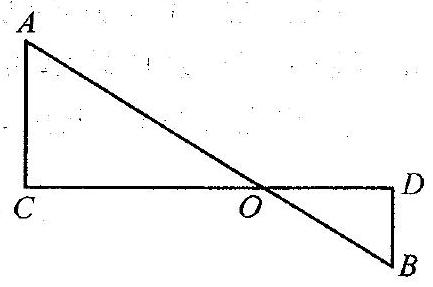
\includegraphics[max width=\textwidth, center]{2024_10_30_26b590fd1106d28139f0g-054}

\section*{心智体操}
病人对牙科医生说:"你真会赚钱,只用三秒就赚了我三个美元。"医生回答说:"如果你愿意的话,我可以按慢动作给你拔。"

差笛何须怨杨浉,\\
春风不度王门关。

\section*{王之涣《凉州词》}
是否所有的一元二次方程都有实数解呢?\\
好像不是,如方程 $x^{2}-x+1=0$ ,通过配方后,它却是 $\left(x-\frac{1}{2}\right)^{2}=-\frac{3}{4}$ ,而这是不可能成立的,这说明此方程无实数解。那么,满足什么条件的方程就一定有实数解呢?

我们已经知道一元二次方程 $a x^{2}+b x+c=0(a \neq 0)$ 可以通过配方转化为

即

\begin{align*}
\begin{aligned}
a\left(x+\frac{b}{2 a}\right)^{2} & =\frac{b^{2}-4 a c}{4 a} \\
\left(x+\frac{b}{2 a}\right)^{2} & =\frac{b^{2}-4 a c}{4 a^{2}}
\end{aligned}
\end{align*}

根据平方根的定义,当 $b^{2}-4 a c \geqslant 0$ 时,方程才有实数根;当 $b^{2}-4 a c<0$时,方程无实数根。人们把 $b^{2}-4 a c$ 称为一元二次方程的判别式,记为 $\Delta$ 。

当 $\Delta=b^{2}-4 a c=0$ 时, $\left(x+\frac{b}{2 a}\right)^{2}=0$ ,那么方程有两个相同的根(称为重根);当 $\Delta=b^{2}-4 a c>0$ 时,方程有两个不同的实数根,分别为

\begin{align*}
x_{1}=\frac{-b+\sqrt{\Delta}}{2 a}, x_{2}=\frac{-b-\sqrt{\Delta}}{2 a}
\end{align*}

由此可知, $\Delta$ 的正负性尤如"玉门关",关联着方程有无实数根。\\
因此说,有方程 $a x^{2}+b x+c=0(a \neq 0)$ 就有 $\Delta$ 。反之有 $\Delta$ ,就可联想到

业务:初高中联赛班、培优班、美国高中数学、教师培训、机构教学产品研发、讲义资料出售等\\
某个一元二次方程。具有了这样的基本意识,往往可以方便解题。\\
上述的求根公式,还可以变形为

\begin{align*}
(2 a x+b)^{2}=b^{2}-4 a c=\Delta,
\end{align*}

这是一个非常有用的等式。\\
例1 已知 $a, b, c$ 是三角形的三边,试判别方程 $b^{2} x^{2}+\left(b^{2}+c^{2}-a^{2}\right) x+$ $c^{2}=0$ 有无实数根?

基本思路 方程的判别式 $\Delta$ 可分解为 $(b-c-a)(b-c+a)(b+c-$ $a)(a+b+c)$ ,利用三角形三边之间的关系,知 $\Delta<0$ 。

解 方程 $b^{2} x^{2}+\left(b^{2}+c^{2}-a^{2}\right) x+c^{2}=0$ 的判别式是

\begin{align*}
\begin{aligned}
\Delta & =\left(b^{2}+c^{2}-a^{2}\right)^{2}-4 b^{2} c^{2} \\
& =(b-c-a)(b-c+a)(b+c-a)(a+b+c)
\end{aligned}
\end{align*}

因为 $a, b, c$ 为三角形的三边,所以

\begin{align*}
b+c>a, a+b>c, c+a>b
\end{align*}

即

\begin{align*}
\cdot b-c-a<0, b-c+a>0, b+c-a>0
\end{align*}

于是 $\Delta<0$, 即方程无实数根。\\
例2 求方程 $x+y=x^{2}-x y+y^{2}+1$ 的实数解。\\
基本思路 二元方程看作关于一个元(如 $x$ )的二次方程,由 $x, y$ 为实数,利用判别式 $\Delta \geqslant 0$ ,得 $-3(y-1)^{2} \leqslant 0$ ,则 $y=1$ ,从而求解出 $x$ 的值。这样的做法是基本的,读者需拥有"多元即少元(如一元)"的意识。

解 方程 $x+y=x^{2}-x y+y^{2}+1$ 可以变形为关于 $x$ 的一元二次方程

\begin{align*}
x^{2}-(y+1) x+\left(y^{2}-y+1\right)=0
\end{align*}

要使得此方程有实数解 $x$ ,则必有

\begin{align*}
\Delta=(y+1)^{2}-4\left(y^{2}-y+1\right)=-3(y-1)^{2} \geqslant 0
\end{align*}

因为

\begin{align*}
-3(y-1)^{2} \leqslant 0
\end{align*}

所以

\begin{align*}
y-1=0 \text {, 即 } y=1 \text {. }
\end{align*}

把 $y=1$ 代入题中方程得

\begin{align*}
\begin{gathered}
x^{2}-2 x+1=0 \\
x=1
\end{gathered}
\end{align*}

解得\\
故方程的实数解为 $x=1, y=1$ 。

业务:初高中联赛班、培优班、美国高中数学、教师培训、机构教学产品研发、讲义资料出售等\\
例3 当 $a, b$ 为何值时,方程

\begin{align*}
x^{2}+2(1+a) x+\left(3 a^{2}+4 a b+4 b^{2}+2\right)=0
\end{align*}

有实数根。\\
基本思路 利用判别式 $\geqslant 0$ ,并将判别式进行配方化简得

\begin{align*}
(a+2 b)^{2}+(a-1)^{2} \leqslant 0
\end{align*}

解 因为原方程有实根,所以

\begin{align*}
\Delta=4(1+a)^{2}-4\left(3 a^{2}+4 a b+4 b^{2}+2\right) \geqslant 0
\end{align*}

得

\begin{align*}
\begin{gathered}
(1+a)^{2}-\left(3 a^{2}+4 a b+4 b^{2}+2\right) \geqslant 0 \\
2 a^{2}+4 a b+4 b^{2}-2 a+1 \leqslant 0 \\
(a+2 b)^{2}+(a-1)^{2} \leqslant 0
\end{gathered}
\end{align*}

即

因为 $(a+2 b)^{2} \geqslant 0,(a-1)^{2} \geqslant 0$, 所以

\begin{align*}
(a+2 b)^{2}+(a-1)^{2} \geqslant 0,
\end{align*}

从而有

\begin{align*}
\begin{gathered}
(a-1)^{2}+(a+2 b)^{2}=0, \text { 得 }\left\{\begin{array}{l}
a-1=0, \\
a+2 b=0
\end{array},\right. \\
a=1, b=-\frac{a}{2}=-\frac{1}{2} .
\end{gathered}
\end{align*}

因此

\section*{051}
故当 $a=1, b=-\frac{1}{2}$ 时,原方程有实根。\\
说明 还可以直接用配方法转化方程。\\
原方程两边都乘以 2 ,并展开,得

\begin{align*}
2 x^{2}+4 x+4 a x+6 a^{2}+8 a b+8 b^{2}+4=0
\end{align*}

配方,得

\begin{align*}
(x+2)^{2}+(x+2 a)^{2}+2(a+2 b)^{2}=0
\end{align*}

因为 $(x+2)^{2},(x+2 a)^{2}, 2(a+2 b)^{2}$ 均非负,所以

\begin{align*}
\begin{aligned}
& (x+2)^{2}=(x+2 a)^{2}=2(a+2 b)^{2}=0, \\
& x=-2, a=-\frac{x}{2}=1, b=-\frac{a}{2}=-\frac{1}{2}
\end{aligned}
\end{align*}

即当 $a=1, b=-\frac{1}{2}$ 时,原方程有实根 $x=-2$ 。

例4 设 $a, b, c$ 是不全相等的实数,三个方程 $a x^{2}+2 b x+c=0, b x^{2}+$ $2 c x+a=0, c x^{2}+2 a x+b=0$ 能同时有相等实数根吗?

基本思路 假设三个方程同时有相等的实数根,则三个判别式同时为 0 ,从而其和也为 0 ,推得 $a=b=c$ 。与题设矛盾。故不可能。

解 若三个方程同时有相等实数根,则三个方程的判别式都为 0 ,即 $4\left(b^{2}-\right.$ $a c)=4\left(c^{2}-a b\right)=4\left(a^{2}-b c\right)=0$ ,所以

\begin{align*}
\begin{aligned}
& 2\left(b^{2}-a c\right)+2\left(c^{2}-a b\right)+2\left(a^{2}-b c\right) \\
= & (a-b)^{2}+(b-c)^{2}+(c-a)^{2}=0,
\end{aligned}
\end{align*}

得 $a=b=c$. 这与条件矛盾. 因此所给方程不能同时有相等实数根.\\
说明 还可如下论述:设三个方程的判别式分别为 $\Delta_{1} 、 \Delta_{2} 、 \Delta_{3}$ ,由 $a, b$ , $c$ 不全相等,得

\begin{align*}
\begin{aligned}
\Delta_{1}+\Delta_{2}+\Delta_{3} & =4\left(b^{2}-a c\right)+4\left(c^{2}-a b\right)+4\left(a^{2}-b c\right) \\
& =2\left[(a-b)^{2}+(b-c)^{2}+(c-a)^{2}\right]>0
\end{aligned}
\end{align*}

所以 $\Delta_{1} 、 \Delta_{2} 、 \Delta_{3}$ 中至少有一个大于 0 ,即至少有一个方程有不等实数根。\\
若在处理问题时,单独处理各个式子有困难,则需有意识"考虑它们的和 (或积)是否易于得到结论?"。

例5 试求出这样的四位数,它的前两位数字与后两位数字分别组成的两位数之和的平方,恰好等于这个四位数。(2003年全国初中数学联赛题)

基本思路 由题设可以得到前两位数 $x$ 与后两位数 $y$ 满足方程 $(x+y)^{2}=$ $100 x+y$ 。然后仿照例 2 求得 $y \leqslant 25$ 。进而考虑 2500 - $99 y$ 在 $y \leqslant 25$ 情形下何时为完全平方数。

解 设前后两个两位数分别为 $x 、 y$ ,则 $10 \leqslant x 、 y \leqslant 99$ 。由题意得

即

\begin{align*}
\begin{gathered}
(x+y)^{2}=100 x+y \\
x^{2}+2(y-50) x+\left(y^{2}-y\right)=0
\end{gathered}
\end{align*}

根据题意,上述关于 $x$ 的方程必有实数解,则有

\begin{align*}
\begin{aligned}
\Delta & =4(y-50)^{2}-4\left(y^{2}-y\right) \\
& =4(2500-99 y) \geqslant 0
\end{aligned}
\end{align*}

即

\begin{align*}
y \leqslant 25
\end{align*}

又 $x, y$ 均为整数,且 $x=50-y \pm \sqrt{2500-99 y}$ ,那么 2500-99y 必是完全平方数,而完全平方数的末位数字仅可能为 $0,1,4,5,6,9$ 。

显然, $y$ 不可能等于 $12,22,13,23,17,18$ ;而对于 $y=11,21,14,24$ ,\\
$15,16,19,10,20$, 都不能使得 $2500-99 y$ 是完全平方数, 所以只有 $y=$ 25 ,此时 $2500-99 y=25$ 。

于是 $x=30$ 或 20 。\\
故所求四位数为 2025 或 3025 。\\
例6 已知 $b^{2}-4 a c$ 是一元二次方程 $a x^{2}+b x+c=0(a \neq 0)$ 的一个实数根,求 $a b$ 的取值范围。(2004 年全国初中数学联赛题)

基本思路 $a x^{2}+b x+c=0$ 可以变形为

\begin{align*}
(2 a x+b)^{2}=b^{2}-4 a c
\end{align*}

分解 $\left(2 a x_{0}+b\right)^{2}=x_{0}$ 得 $2 a x_{0}+b=\sqrt{x_{0}}$, 或 $2 a x_{0}+b=-\sqrt{x_{0}}$ (这里 $\left.x_{0}=b^{2}-4 a c\right)$ ,从而得到 $1-8 a b=\left(4 a \sqrt{x_{0}}-1\right)^{2}$ ,或 $\left(4 a \sqrt{x_{0}}+1\right)^{2}$ 。

解 令 $x_{0}=b^{2}-4 a c$ 是方程 $a x^{2}+b x+\dot{c}=0$ 的实根,则由 $b^{2}-4 a c \geqslant 0$得 $x_{0} \geqslant 0$, 并且

\begin{align*}
\left(2 a x_{0}+b\right)^{2}=b^{2}-4 a c
\end{align*}

即

\begin{align*}
\left(2 a x_{0}+b\right)^{2}=x_{0}
\end{align*}

得

\begin{align*}
\left[\left(2 a x_{0}+b\right)-\sqrt{x_{0}}\right]\left[\left(2 a x_{0}+b\right)+\sqrt{x_{0}}\right]=0,
\end{align*}

即

\begin{align*}
2 a x_{0}+b=\sqrt{x_{0}} \text { 或 } 2 a x_{0}+b=-\sqrt{x_{0}} \text {. }
\end{align*}

由 $2 a x_{0}+b-\sqrt{x_{0}}=0$ 得

\begin{align*}
\left(4 a \sqrt{x_{0}}-1\right)^{2}-(1-8 a b)=0,
\end{align*}

即

\begin{align*}
1-8 a b=\left(4 a \sqrt{x_{0}}-1\right)^{2} \geqslant 0
\end{align*}

由 $2 a x_{0}+b+\sqrt{x_{0}}=0$ 得

\begin{align*}
\left(4 a \sqrt{x_{0}}+1\right)^{2}-(1-8 a b)=0
\end{align*}

即

\begin{align*}
1-8 a b=\left(4 a \sqrt{x_{0}}+1\right)^{2} \geqslant 0
\end{align*}

所以 $1-8 a b \geqslant 0$, 即 $a b \leqslant \frac{1}{8}$ ,且当 $b^{2}-4 a c=\frac{1}{16 a^{2}}$ 时,等号成立。如当 $a=\frac{1}{2}, b=\frac{1}{4}, c=-\frac{3}{32}$ 时, 就满足题中要求.

故 $a b$ 的取值范围为 $a b \leqslant \frac{1}{8}$.\\
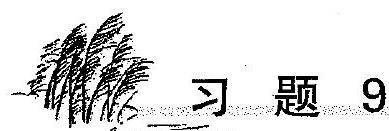
\includegraphics[max width=\textwidth, center]{2024_10_30_26b590fd1106d28139f0g-060}

11 是什么实数时,方程 $k x^{2}-(2 k+1) x+k=0$ 有两个不相等的实数根?\\
2: 已知方程 $2 x(k x-4)-x^{2}+6=0$ 无实数根,求 $k$ 的取值范围。\\
31 已知关于 $x$ 的方程 $x^{2}-2 \sqrt{-a} x+\frac{(a-1)^{2}}{4}=0$ 有实数根,其中 $a$ 为实数,求 $a^{2012}-x^{2012}$ 的值。\\
4 . 对于实数 $u, v$ ,定义一种运算"*"为: $u * v=u v+v$ 。若关于 $x$ 的方程 $x *$ $(a * x)=-\frac{1}{4}$ 有两个不同的实数根,求实数 $a$ 的取值范围。(2008年全国初中数学竞赛题)\\
5 已知关于 $x, y$ 的方程 $5 x^{2}-3 x y+\frac{1}{2} y^{2}-2 x+\frac{1}{2} y+\frac{1}{4}=0$, 求它的实数解。\\
6. 已知三角形的三边的长为 $a, b, c$ ,且方程 $(c-b) x^{2}+2(b-a) x+a-b=$ 0 有两个相等的实数根,试判断此三角形的形状。\\
47 在 $\triangle A B C$ 中, $A B=A C=m, B C=n$ ,求证:方程 $4 x^{2}-8 m x+n^{2}=0$有两个不相等的实数根。\\
8. 已知关于 $x$ 的方程 $x^{2}-(2 k+1) x+4\left(k-\frac{1}{2}\right)=0$ 。\\
(1)求证:无论 $k$ 取什么实数值,这个方程总有实数根;\\
(2)如果等腰三角形的一腰和底边长分别是这个方程的两个根,求实数 $k$的取值范围。

\section*{山智盾操}
\section*{一声公鸡叫}
俄国著名生物学教授弗 $\cdot$ 奥 $\cdot$ 格瓦列夫在一次讲课时,有个家伙故意捣乱,突然学起了公鸡啼叫,顿时,引起哄堂大笑。

教授不动声色地看了一下自己的怀表,说:"我的这只表误时了,没想到现在已是凌晨。不过,同学们请相信我的话,公鸡报晓是低等动物的一种本能."

湖光秋月两相和,潭面无风镜未磨。遥望洞庭山水色,白银盘里一青螺

刘禹锡《望洞庭》

在前面我们已经认识并了解了一元二次方程与方程的根的关系。\\
我们知道,方程是由系数、未知数及未知数的次数构成的,也就是说,一元二次方程可以认为由各项的系数所决定,如二次项、一次项和常数项系数分别为 $2 、 3 、-4$ ,那么这个一元二次方程就被确定了,即是 $2 x^{2}+$ $3 x-4=0$ 。

自然地,这就引发我们去思考,方程的根与方程的系数有怎样的关系呢?让我们共同来探求吧。

如果一元二次方程 $a x^{2}+b x+c=0(a \neq 0)$ 的两根为 $x_{1}, x_{2}$, 那么就有

\begin{align*}
a x^{2}+b x+c=a\left(x-x_{1}\right)\left(x-x_{2}\right)
\end{align*}

比较等式两边对应项的系数,得

\begin{align*}
\left\{\begin{array}{l}
x_{1}+x_{2}=-\frac{b}{a}  \tag{1}\\
x_{1} x_{2}=\frac{c}{a}
\end{array}\right.
\end{align*}

(1)式与(2)式也可以运用求根公式得到。

上述公式(1)与(2),人们称之为韦达定理,即根与系数的关系。\\
因此,我们知道,给定一元二次方程 $a x^{2}+b x+c=0(a \neq 0)$ 就一定有(1)式与(2)式成立。\\
10. 根与宗数的关系及其应用

物理竞赛群:271751860,化学竞赛群:271751511,生物竞赛群:254139830,信息竞赛群:281798334,英语竞赛群:271750414,英语口语群:168570356,心算交流群:131033273,厦门培训机构教师招聘

业务:初高中联赛班、培优班、美国高中数学、教师培训、机构教学产品研发、讲义资料出售等\\
反过来,如果有两数 $x_{1}, x_{2}$ 满足(1)式与(2)式,那么这两数 $x_{1}, x_{2}$ 必是一个一元二次方程 $a x^{2}+b x+c=0$ 的根。利用这一基本知识常可以简捷地处理问题。

利用根与系数的关系,我们可以不求方程 $a x^{2}+b x+c=0$ 的根,而知其根的正、负性。

在 $\Delta=b^{2}-4 a c \geqslant 0$ 的条件下,我们有如下结论:\\
当 $\frac{c}{a}<0$ 时,方程的两根必一正一负. 若 $-\frac{b}{a} \geqslant 0$, 则此方程的正根不小于负根的绝对值; 若 $-\frac{b}{a}<0$, 则此方程的正根小于负根的绝对值.

当 $\frac{c}{a}>0$ 时,方程的两根同正或同负。若 $-\frac{b}{a}>0$, 则此方程的两根均为正根;若 $-\frac{b}{a}<0$ ,则此方程的两根均为负根。

恰是一元二次方程如"银盘",根与系数总"相和"。\\
例1 设 $x_{1}, x_{2}$ 是方程 $x^{2}-2(k+1) x+k^{2}+2=0$ 的两个实数根,且 $\left(x_{1}+1\right)\left(x_{2}+1\right)=8$ ,求 $k$ 的值。

基本思路 由判别式得 $k$ 的取值范围,由根与系数关系及题设得方程 $k^{2}+2 k-3=0$.

解 由题意得

\begin{align*}
\Delta=[-2(k+1)]^{2}-4\left(k^{2}+2\right) \geqslant 0
\end{align*}

得 $k \geqslant \frac{1}{2}$.\\
又 $x_{1}+x_{2}=2(k+1), x_{1} x_{2}=k^{2}+2$, 那么

\begin{align*}
\left(x_{1}+1\right)\left(x_{2}+1\right)=x_{1} x_{2}+\left(x_{1}+x_{2}\right)+1=8
\end{align*}

即

\begin{align*}
\begin{gathered}
k^{2}+2+2(k+1)+1=8 \\
k^{2}+2 k-3=0 \\
k_{1}=-3, k_{2}=1
\end{gathered}
\end{align*}

解得\\
但 $k_{1}=-3$ 不满足 $k \geqslant \frac{1}{2}$ ,所以 $k=1$ 。\\
说明 上述讨论的前提是方程有实数根,所以一定要注意满足判别式,否则就会得到不正确的结果。

例 2 已知 $x_{1}, x_{2}$ 是方程 $x^{2}-2 m x+\left(m^{2}+2 m+3\right)=0$ 的两个实数根,求 $x_{1}^{2}+x_{2}^{2}$ 的最小值。

基本思路 同例 1 ,别忘由判别式得 $m$ 的范围,然后用根与系数关系得到 $x_{1}^{2}+x_{2}^{2}=2 m^{2}-4 m-6$ ,配方后求得结果。

解 由题意知

\begin{align*}
\Delta=(-2 m)^{2}-4 \times\left(m^{2}+2 m+3\right) \geqslant 0
\end{align*}

得

\begin{align*}
m \leqslant-\frac{3}{2}
\end{align*}

又 $x_{1}+x_{2}=2 m, x_{1} x_{2}=m^{2}+2 m+3$, 则

\begin{align*}
\begin{aligned}
& x_{1}^{2}+x_{2}^{2} \\
= & \left(x_{1}+x_{2}\right)^{2}-2 x_{1} x_{2} \\
= & 4 m^{2}-2\left(m^{2}+2 m+3\right) \\
= & 2 m^{2}-4 m-6 \\
= & 2\left[(m-1)^{2}-4\right] .
\end{aligned}
\end{align*}

由 $m \leqslant-\frac{3}{2}, m-1 \leqslant-\frac{5}{2}$, 则

所以

\begin{align*}
\begin{aligned}
(m-1)^{2} & \geqslant\left(-\frac{5}{2}\right)^{2}=\frac{25}{4} \\
x_{1}^{2}+x_{2}^{2} & =2\left[(m-1)^{2}-4\right] \\
& \geqslant 2 \times \frac{25}{4}-8 \\
& =\frac{9}{2}
\end{aligned}
\end{align*}

故 $x_{1}^{2}+x_{2}^{2}$ 的最小值为 $\frac{9}{2}$ ,此时 $m=-\frac{3}{2}$ 。\\
说明 用配方来求二次式的最大值 (最小值),是初中求一类最值问题的基本技巧。

例3 如图 10-1, 过正方形 $A B C D$ 的顶点 $C$ 任作一条直线与 $A B 、 A D$ 的延长线分别相交于点 $P 、 Q$. 求证: $A P+A Q \geqslant 2 \sqrt{2} B D$ 。

基本思路 不妨设 $A B C D$ 边长为 $a$ ,观察图形可知

\begin{align*}
S_{\triangle A P Q}=S_{\triangle A P C}+S_{\triangle A Q C}
\end{align*}

由面积公式得\\
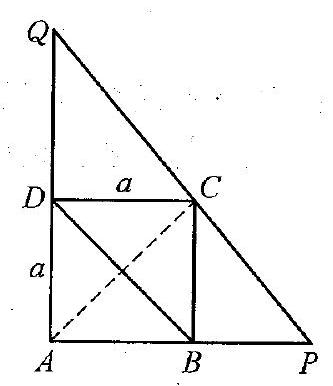
\includegraphics[max width=\textwidth, center]{2024_10_30_26b590fd1106d28139f0g-063}

图 10-1

业务:初高中联赛班、培优班、美国高中数学、教师培训、机构教学产品研发、讲义资料出售等

\begin{align*}
\begin{gathered}
\frac{1}{2} A P \cdot A Q=\frac{1}{2} a \cdot A P+\frac{1}{2} a \cdot A Q, \\
A P \cdot A Q=a(A P+A Q) .
\end{gathered}
\end{align*}

即\\
因此可构造以 $A P 、 A Q$ 为根的一元二次方程,并通过 $\Delta \geqslant 0$ 来证明结论。\\
解 由题设可知 $S_{\triangle A P Q}=S_{\triangle A P C}+S_{\triangle A Q C}$ ,得

即

\begin{align*}
\begin{gathered}
\frac{1}{2} A P \cdot A Q=\frac{1}{2} a \cdot A P+\frac{1}{2} a \cdot A Q \\
A P \cdot A Q=a(A P+A Q)
\end{gathered}
\end{align*}

于是,可以将 $A P 、 A Q$ 看作是方程

\begin{align*}
x^{2}-(A P+A Q) x+a(A P+A Q)=0
\end{align*}

的两个实根,所以判别式

\begin{align*}
\Delta=(A P+A Q)^{2}-4 a(A P+A Q) \geqslant 0
\end{align*}

即

\begin{align*}
A P+A Q \geqslant 4 a
\end{align*}

因为在正方形 $A B C D$ 中, $B D=\sqrt{A B^{2}+A D^{2}}=\sqrt{a^{2}+a^{2}}=\sqrt{2} a$, 所以 $a=\frac{\sqrt{2}}{2} B D$ ,从而有

\begin{align*}
A P+A Q \geqslant 4 \cdot \frac{\sqrt{2}}{2} B D=2 \sqrt{2} B D
\end{align*}

例4 已知方程 $x^{2}-3 x+2-k^{2}=0, k$ 为实数,且 $k \neq 0$ ,证明:此方程有两个实数根,其中一根大于 1 ,另一根小于 1 。

基本思路 先计算判别式大于 0 ,后考虑 $(\alpha-1)(\beta-1)$ 是否小于 0 。\\
解 因为方程 $x^{2}-3 x+2-k^{2}=0$ 的判别式

\begin{align*}
\Delta=(-3)^{2}-4\left(2-k^{2}\right)=1+4 k^{2}>0
\end{align*}

所以方程有两个不同的实数根,不妨设为 $\alpha, \beta$ ,且 $\alpha \neq \beta$ 。\\
由根与系数关系得

\begin{align*}
\begin{aligned}
\alpha+\beta=3 & , \alpha \beta=2-k^{2} \\
(\alpha-1)(\beta-1) & =\alpha \beta-(\alpha+\beta)+1 \\
& =2-k^{2}-3+1 \\
& =-k^{2}<0,(k \neq 0)
\end{aligned}
\end{align*}

\begin{center}

\includegraphics[max width=\textwidth]{2024_10_30_26b590fd1106d28139f0g-064}
\end{center}

物理竞赛群:271751860,化学竞赛群:271751511,生物竞赛群:254139830,信息竞赛群:281798334,英语竞赛群:271750414,英语 $\square$ 语群:168570356,心算交流群:131033273,厦门培训机构教师招聘

业务:初高中联赛班、培优班、美国高中数学、教师培训、机构教学产品研发、讲义资料出售等\\
则有 $\alpha-1$ 与 $\beta-1$ 中必有一个大于 0 ,另一个小于 0.\\
于是可知 $\alpha$ 与 $\beta$ 中一个大于 1 ,另一个小于 1 。\\
说明 本题也可转化方程为 $y^{2}-y-k^{2}=0$ (这里 $y=x-1$ )直接讨论。\\
例 5 解方程

\begin{align*}
(\sqrt{2+\sqrt{3}})^{x}+(\sqrt{2-\sqrt{3}})^{x}=4
\end{align*}

基本思路 换元转化为 $a+b=4$ ,且 $a b=1$ ,从而转化为方程 $t^{2}-4 t+$ $I=0$ 的求解,回代得结果。

解 因为 $(2+\sqrt{3})(2-\sqrt{3})=1$, 则令 $(\sqrt{2+\sqrt{3}})^{x}=a,(\sqrt{2-\sqrt{3}})^{x}=$ $b$ ,有

\begin{align*}
\left\{\begin{array}{l}
a+b=4, \\
a b=1
\end{array}\right.
\end{align*}

所以 $a, b$ 是方程 $t^{2}-4 t+1=0$ 的两个实数根,解得 $t=2 \pm \sqrt{3}$ ,即

\begin{align*}
\begin{gathered}
(\sqrt{2+\sqrt{3}})^{x}=2 \pm \sqrt{3}, \\
x=2 \text { 或 } x=-2 .
\end{gathered}
\end{align*}

解得\\
说明 此题还可采用换元法令 $y=(\sqrt{2+\sqrt{3}})^{x}$ 得到结果.\\
例6 实数 $a, b, c$ 满足 $a \leqslant b \leqslant c$ ,且 $a b+b c+c a=0, a b c=1$ 。求最大的实数 $k$ ,使得不等式

\begin{align*}
|a+b| \geqslant k|c|
\end{align*}

恒成立。(2007 年全国初中数学竞赛题)\\
基本思路 将 $a, b$ 看作方程 $x^{2}+\frac{1}{c^{2}} x+\frac{1}{c}=0$ 的两个实根,从而有判别式 $\Delta \geqslant 0$ ,进而推得 $|a+b| \geqslant 4|c|$ (这里易知 $c>0$ ),且等号当且仅当 $c=$ $\frac{\sqrt[3]{2}}{2}, a=b=-\sqrt[3]{2}$ 时成立,故 $k$ 的最大值为 4 。

解 由已知条件知, $a, b, c$ 都不等于 0 , 且 $c>0$.\\
因为 $a b=\frac{1}{c}>0, a+b=-\frac{1}{c^{2}}<0$ ,所以 $a \leqslant b<0$ 。\\
由一元二次方程根与系数的关系知, $a, b$ 是一元二次方程

\begin{align*}
x^{2}+\frac{1}{c^{2}} x+\frac{1}{c}=0
\end{align*}

业务:初高中联赛班、培优班、美国高中数学、教师培训、机构教学产品研发、讲义资料出售等\\
的两个实数根,于是

所以

\begin{align*}
\begin{gathered}
\Delta=\frac{1}{c^{4}}-\frac{4}{c} \geqslant 0 \\
c^{3} \leqslant \frac{1}{4} .
\end{gathered}
\end{align*}

因此

\begin{align*}
|a+b|=-(a+b)=\frac{1}{c^{2}} \geqslant 4 c=4|c|
\end{align*}

等号只有当 $c=\frac{\sqrt[3]{2}}{2}, \Delta=0$ ,得 $a=b=-\sqrt[3]{2}$ 时成立。\\
故 $k$ 的最大值为 4.\\
例7 已知 $a, b, c$ 为实数,且 $a>0, b^{2}-a c<0, x_{1}, x_{2}$ 是方程 $x^{2}-$ $(a+c) x-b^{2}+a c=0$ 的两个实数根。证明:\\
(1) $x_{1}, x_{2}$ 都是正数;\\
(2)若 $x_{1} \geqslant x_{2}$ ,则 $x_{1} \geqslant a , x_{2} \leqslant c$ 。\\
基本思路 由题设推得 $c>0$. 注意到方程右边的式子可以是 $\left(x-x_{1}\right)$ $\left(x-x_{2}\right)$ ,令 $x=a$ 和 $x=c$ ,得其积式的正负性。

证明(1)因为 $a>0, b^{2}-a c<0$ ,即 $0 \leqslant b^{2}<a c$ ,所以 $c>0$ 。由根与系数的关系得

\begin{align*}
\begin{gathered}
x_{1}+x_{2}=a+c>0, \\
x_{1} x_{2}=-b^{2}+a c>0 .
\end{gathered}
\end{align*}

由此可知方程两根 $x_{1}, x_{2}$ 都是正数。\\
(2)因为方程的两根为 $x_{1}, x_{2}$ ,则有

于是

\begin{align*}
x_{1}+x_{2}=a+c, x_{1} x_{2}=-b^{2}+a c,
\end{align*}

\begin{align*}
\left(a-x_{1}\right)\left(a-x_{2}\right)=-b^{2} \leqslant 0
\end{align*}

又 $x_{1} \geqslant x_{2}$, 则 $x_{2} \leqslant a \leqslant x_{1}$.\\
同样地,有

\begin{align*}
\left(c-x_{1}\right)\left(c-x_{2}\right)=-b^{2} \leqslant 0
\end{align*}

则由 $x_{1} \geqslant x_{2}$. 得

\begin{align*}
x_{2} \leqslant c \leqslant x_{1}
\end{align*}

故结论成立。

\section*{习 题 10}
I 已知 $6 a^{2}-100 a+7=0$ 及 $7 b^{2}-100 b+6=0$ ,且 $a b \neq 1$ ,求 $\frac{a}{b}$ 的值。\\
2. 已知方程 $(1999 x)^{2}-1998 \times 2000 x-1=0$ 的较大根为 $m, x^{2}+1998 x-1999$ $=0$ 的较小根为 $n$, 求 $m-n$ 的值。\\
3 已知 $m^{2}+71 m-1999=0, n^{2}+71 n-1999=0$, 且 $m \neq n$, 求 $\frac{1}{m}+\frac{1}{n}$ 的值.

4 已知一元二次方程 $x^{2}-4 a x+5 a^{2}-6 a=0$ 有两个实根,且两根之差的绝对值为 6 ,求 $a$ 的值。\\
$5 a$ 为何值时,方程 $(a+1) x^{2}+(a-5) x+(a+6)=0$ 的一个根比另一个根的 2 倍小 1 ?\\
26 已知方程 $x^{2}-2 a x+\left(a^{2}-a+6\right)=0$ 的两个根为 $\alpha, \beta$, 试求 $(\alpha-1)^{2}+$ $(\beta-1)^{2}$ 的最小值。\\
7 已知实数 $x, y, z$ 满足 $x+y=5$ 及 $z^{2}=x y+y-9$, 求 $x+2 y+3 z$ 的值. 8 已知 $\alpha, \beta$ 是方程 $x^{2}-x-1=0$ 的两根,求 $\alpha^{4}+3 \beta$ 的值。\\
9 设 $a$ 是正实数,求证:方程 $\frac{1}{x}+\frac{1}{x+a}+\frac{1}{x+a^{2}}=0$ 有两个同号的实数根。\\
10 设 $a$ 是实数,已知 $x$ 的二次方程 $x^{2}-2 a x+a^{2}-4=0$ 。\\
(1) $a$ 为何值时,方程有两个正根?\\
(2) $a$ 为何值时,方程有一正根、一负根?

\section*{L稫体操}
我给你一根金色线头,\\
绕成一个球形,\\
她就将把你引领到,\\
天堂之门…..\\
——[英]W. Blake (1757-1827)

10 根与系数的关亮及其应用

物理竞赛群:271751860,化学竞赛群:271751511,生物竞赛群:254139830,信息竞赛群:281798334,英语竞赛群:271750414,英语口语群:168570356,心算交流群:131033273,厦门培训机构教师招聘

踢足球,首要的且必须的是,学会玩足球……\\
——中国前国家足球队教练 米卢

让我们一起来玩"魔术"吧!\\
看着方程 $x^{2}-x-6=0$ ,即

\begin{align*}
(x+2)(x-3)=0
\end{align*}

想你所想,即变。\\
想 1 式子 $x+2$ 换为 $x^{2}-2$ ,方程如何?\\
得方程 $\left(x^{2}-2\right)(x-3)=0$ ,即为三次方程

\begin{align*}
x^{3}-3 x^{2}-2 x+6=0 \tag{1}
\end{align*}

想 2 式子 $x+2$ 换为 $x^{2}-2 x-15$ ,方程如何?\\
得方程 $\left(x^{2}-2 x-15\right)(x-3)=0$ ,即为三次方程

\begin{align*}
x^{3}-5 x^{2}-9 x+45=0 \tag{2}
\end{align*}

想 3 式子 $(x+2)(x-3)$ 中的 $x$ 换为 $x^{2}$ ,方程如何?\\
得方程 $\left(x^{2}+2\right)\left(x^{2}-3\right)=0$ ,即为四次方程

\begin{align*}
x^{4}-x^{2}-6=0 \tag{3}
\end{align*}

想 4 式子 $(x+2)$ 中的 $x$ 换为 $x^{2}-x$ ,式子 $(x-3)$ 中的 $x$ 换为 $x^{2}+2 x$ ,方程如何?

得方程 $\left(x^{2}-x+2\right)\left(x^{2}+2 x-3\right)=0$ ,即为四次方程

\begin{align*}
x^{4}+x^{3}-3 x^{2}+7 x-6=0 \tag{4}
\end{align*}

想 5 式子 $(x+2)(x-3)$ 中的 $x$ 换为 $x+\frac{1}{x}$, 方程如何?

物理竞赛群:271751860,化学竞赛群:271751511,生物竞赛群:254139830,信息竞赛群:281798334,英语竞赛群:271750414,英语口语群:168570356,心算交流群:131033273,厦门培训机构教师招聘

\begin{align*}
\begin{aligned}
&\left(x+\frac{1}{x}+2\right)\left(x+\frac{1}{x}-3\right)=0 \text {, 即为方程 } \\
&\left(x^{2}+\frac{1}{x^{2}}\right)-\left(x+\frac{1}{x}\right)-4=0,
\end{aligned}
\end{align*}

即

\begin{align*}
x^{4}-x^{3}-4 x^{2}-x+1=0 \tag{5}
\end{align*}

你还可以继续想下去,变下去,就会得到许多许多你能够解决的,但你可能未曾见过的方程。

上述方程(1)~(5),都是涉及三次或三次以上多项式的方程,又叫做高次方程。

如何解这些高次方程呢?

\section*{回头看"来路"。}
对于多项式方程(1)、(2)可以运用因式分解,把它们化为一次方程、二次方程的积,即将这样的多项式方程转化为一次方程和二次方程。

对于多项式方程(3),又叫做双二次方程,只需直接将 $x^{2}$ 看作 $y$ ,转化方程为二次方程。

对于多项式方程(4),可以考虑用因式分解,但有一定的难度,通常可以考虑用待定系数法,即设

\begin{align*}
x^{4}+x^{3}-3 x^{2}+7 x-6=\left(x^{2}+a x+b\right)\left(x^{2}+c x+d\right),
\end{align*}

结合恒等式的性质,尝试求得 $a, b, c, d$ ,从而转化方程为二次方程。\\
对于多项式方程(5),又叫做倒数方程,考虑将方程的两端同时除以 $x^{2}$ 后,运用换元把原方程转化为会解的方程。\\
"实践出真知",让我们一起来实践对上述方程求解的认识。\\
例1 解方程 $x^{3}-3 x+2=0$ 。\\
基本思路 观察方程后知方程左边系数的和是 0 ,则有因式 $x-1$ 。从而将方程转化为 $x-1=0$ ,或 $x^{2}+x-2=0$ 。易求得结果。

解 原方程可化为

得

\begin{align*}
\begin{aligned}
& \left(x^{3}-1\right)-3(x-1)=0 \\
& (x-1)\left(x^{2}+x-2\right)=0
\end{aligned}
\end{align*}

即

\begin{align*}
(x-1)(x+2)(x-1)=0
\end{align*}

解得

\begin{align*}
x_{1}=x_{2}=1, x_{3}=-2
\end{align*}

说明 对于高次方程,如果方程中各项的系数和是 0 ,那么这个方程必有根是 1 。通常首先观察 $x=1$ 或 $x=-1$ 是否是高次方程的根,若是,则可以容

易地转化方程为已会解的方程。

例2 若关于 $x$ 的方程 $(x-2)\left(x^{2}-4 x+m\right)=0$ 有三个实数根,且这三个根恰好可以作为一个三角形的三条边的长,则 $m$ 的取值范围是 $\qquad$。 (2011 全国初中数学竞赛题)

基本思路 转化为考虑方程 $x^{2}-4 x+m=0$ 的两根 $x_{1}, x_{2}$ 满足 $\mid x_{1}-$ $x_{2} \mid<2$, 得 $\Delta \geqslant 0$ ,且 $\sqrt{\Delta}<2$ ,从而求得 $m$ 的范围。

解 易知 $x=2$ 是方程的一个根,设方程的另外两个根为 $x_{1}, x_{2}$ ,则 $x_{1}$ , $x_{2}$ 是方程 $x^{2}-4 x+m=0$ 的两个实数根,于是有 $x_{1}+x_{2}=4, x_{1} x_{2}=m$ 。又显然 $x_{1}+x_{2}=4>2$ ,所以有

\begin{align*}
\Delta=16-4 m \geqslant 0, \text { 且 }\left|x_{1}-x_{2}\right|<2 .
\end{align*}

而由求根公式(或根与系数关系)得 $\left|x_{1}-x_{2}\right|=\frac{\sqrt{(-4)^{2}-4 m}}{1}=$ $\sqrt{16-4 m}$ ,因此有 $0 \leqslant 16-4 m<4$ ,解得 $3<m \leqslant 4$ 。

故所求 $m$ 的取值范围是 $3<m \leqslant 4$ 。\\
说明 若题中方程变形为 $x^{3}-6 x^{2}+(m+8) x-2 m=0$ ,则需先发现 $x=2$ 为其一根。

例3 解方程 $x^{4}+(x-4)^{4}=626$ 。\\
基本思路 设法将上述方程通过换元 $y=\frac{x+(x-4)}{2}=x-2$ ,转化题中方程为 $y^{4}+24 y^{2}-297=0$ ,即为双二次方程。

解 利用对称性, 取 0 与 4 的平均数来设元, 即设 $x=y+2$, 则

\begin{align*}
x-4=y-2
\end{align*}

于是方程化为

\begin{align*}
(y+2)^{4}+(y-2)^{4}=626
\end{align*}

即

\begin{align*}
y^{4}+24 y^{2}-297=0
\end{align*}

因式分解得

\begin{align*}
\left(y^{2}-9\right)\left(y^{2}+33\right)=0
\end{align*}

又 $y^{2}=-33$ 无实数解, 所以 $y^{2}=9$, 即 $y= \pm 3$, 从而 $x=5$ 或 $x=-1$.故方程的解为 $x=5$ 或 $x=-1$ 。\\
说明 遇到类似于例 3 的方程

\begin{align*}
(x+a)^{4}+(x+b)^{4}=c,
\end{align*}

常换元为 $(y-d)^{2}+(y+d)^{2}=c$, 则需待定 $\left\{\begin{array}{l}y-d=x+a, \\ y+d=x+b,\end{array}\right.$ 得 $d=\frac{b-a}{2}$, 从

而令 $y=\frac{2 x+a+b}{2}$ 代换简化问题.\\
例 4 解方程 $2 x^{4}+3 x^{3}-16 x^{2}+3 x+2=0$.\\
解 观察方程特点,发现方程中各项系数关于中间项对称。\\
由原方程可知 $x \neq 0$, 则在方程两边同除以 $x^{2}$ ,得

令

\begin{align*}
2\left(x^{2}+\frac{1}{x^{2}}\right)+3\left(x+\frac{1}{x}\right)-16=0
\end{align*}

\begin{align*}
x+\frac{1}{x}=y
\end{align*}

则

\begin{align*}
y^{2}=x^{2}+\frac{1}{x^{2}}+2
\end{align*}

即

\begin{align*}
x^{2}+\frac{1}{x^{2}}=y^{2}-2
\end{align*}

于是上述方程化为

\begin{align*}
2 y^{2}+3 y-20=0
\end{align*}

解这个方程得

\begin{align*}
y=\frac{5}{2} \text { 或 } y=-4 .
\end{align*}

当 $y=\frac{5}{2}$ 时, $x+\frac{1}{x}=\frac{5}{2}$,\\
即

\begin{align*}
\begin{aligned}
& 2 x^{2}-5 x+2=0 \\
& x_{1}=\frac{1}{2}, x_{2}=2 .
\end{aligned}
\end{align*}

当 $y=-4$ 时, $x+\frac{1}{x}=-4$,\\
即

\begin{align*}
x^{2}+4 x+1=0
\end{align*}

解得

\begin{align*}
x_{3}=-2-\sqrt{3}, x_{4}=-2+\sqrt{3}
\end{align*}

所以,原方程的解为

\begin{align*}
x_{1}=\frac{1}{2}, x_{2}=2, x_{3}=-2-\sqrt{3}, x_{4}=-2+\sqrt{3}
\end{align*}

说明 类似于例 4 的方程称为倒数方程,解这样的方程通常运用例 4 的解法求得结果。

你能运用其他思路求解方程 $2 x^{4}+3 x^{3}-16 x^{2}+3 x+2=0$ 吗 $?$

业务:初高中联赛班、培优班、美国高中数学、教师培训、机构教学产品研发、讲义资料出售等\\
例 5 解方程

\begin{align*}
(x-2)(x+1)(x+4)(x+7)=19
\end{align*}

基本思路 利用对等性,配对相乘 $(x-2)(x+7),(x+1)(x+4)$ ,整体代换 $y=x^{2}+5 x-5$ ,转化为 $y^{2}=100$ 。

解 两两相乘,考虑整体代换。

\begin{align*}
\begin{gathered}
{[(x-2)(x+7)][(x+1)(x+4)]=19} \\
\left(x^{2}+5 x-14\right)\left(x^{2}+5 x+4\right)=19
\end{gathered}
\end{align*}

令 $y=\frac{\left(x^{2}+5 x-14\right)+\left(x^{2}+5 x+4\right)}{2}=x^{2}+5 x-5$, 则有

\begin{align*}
(y-9)(y+9)=19,
\end{align*}

即

\begin{align*}
y^{2}-81=19,
\end{align*}

解得

\begin{align*}
y_{1,2}= \pm 10
\end{align*}

当 $y=10$ 时, $x^{2}+5 x-5=10$, 解得 $x_{1,2}=\frac{-5 \pm \sqrt{85}}{2}$;\\
当 $y=-10$ 时, $x^{2}+5 x-5=-10$, 解得 $x_{3,4}=\frac{-5 \pm \sqrt{5}}{2}$.\\
所以原方程的解是

\begin{align*}
x_{1,2}=\frac{-5 \pm \sqrt{85}}{2}, x_{3,4}=\frac{-5 \pm \sqrt{5}}{2}
\end{align*}

例 6 关于 $x$ 的方程 $x^{3}-a x^{2}-2 a x+a^{2}-1=0$ 只有一个实数根,求 $a$的取值范围。

基本思路 转换角度看作是关于 $a$ 的一元二次方程。尝试分解因式发现有 $a=x-1, a=x^{2}+x+1$ 。

解 原方程因式分解得

\begin{align*}
[a-(x-1)]\left[a-\left(x^{2}+x+1\right)\right]=0,
\end{align*}

解得

\begin{align*}
a=x-1 \text { 或 } a=x^{2}+x+1 \text {. }
\end{align*}

于是

\begin{align*}
x=a+1 \text { 或 } x^{2}+x+(1-a)=0 \text {. }
\end{align*}

因为原方程仅有一个实数根,所以方程 $x^{2}+x+(1-a)=0$ 必无实数根,从而有

\begin{align*}
\Delta=1-4(1-a)<0,
\end{align*}

业务:初高中联赛班、培优班、美国高中数学、教师培训、机构教学产品研发、讲义资料出售等

解得

\begin{align*}
a<\frac{3}{4} .
\end{align*}

故符合题意的 $a$ 的取值范围为 $a<\frac{3}{4}$.\\

\includegraphics[max width=\textwidth, center]{2024_10_30_26b590fd1106d28139f0g-073}

1 解方程 $(x+3)\left(x^{2}-5 x+6\right)=0$.\\
2 解方程 $x^{3}+3 x^{2}+4 x+2=0$ 。\\
53 解方程 $(x+1)^{4}+(x+3)^{4}-82=0$.\\
4 求方程 $x^{4}+3 x^{2}+2 x+3=0$ 的实数解的个数。\\
【5 解方程 $2 x^{4}-5 x^{3}+4 x^{2}-5 x+2=0$.\\
6解方程 $6 x^{4}-25 x^{3}+12 x^{2}+25 x+6=0$.\\
47 解方程 $\left(x^{2}-x-1\right)^{x+2}=1$ 。\\
8 已知方程 $a x^{2}+b x+c=x(a>0)$ 的两个实数根 $x_{1}, x_{2}$ 满足 $0<x_{1}<$ $x_{2}<\frac{1}{a}$. 当 $0<x<x_{1}$ 时,证明: $x<a x^{2}+b x+c<x_{1}$.

\section*{心智体操}
\section*{别在自己头脑中挂上鸟笼}
一位心理学家曾和乔打赌说:"如果给你一个鸟笼,并挂在你房中,那么你就一定会买一只鸟。"乔同意打赌。因此,心理学家就买了一只非常漂亮的瑞士鸟笼给他,乔把鸟笼挂在起居室靠近桌子的上头。结果出现的情况是,当人们走进来时就问:"乔,你的鸟什么时候死了?"乔立刻回答:"我从未有过一只鸟。""那么,你要一只鸟笼干吗?"乔不得不解释一番。

后来,只要有人走进乔的屋里,就会问同样的问题。乔的心情因此搞得很烦躁,为了不再让人询问,乔干脆买了一只鸟装进了鸟笼里。

心里学家后来说,去买一只鸟比解释为什么他有一只空鸟笼要简便得多。人们经常是首先在自己头脑中挂上鸟笼,最后就不得不在鸟笼中装上些什么东西。

全国小学奥数群:221739457,全国初中奥数学生群:253736211,全国高中奥数学生群591782992全国初中奥数教练群112464128,全国高中奥数教练群195949359竞赛公众号:新浪微博@郑剑雄 微信:v136257437 QQ:136257437\\
业务:初高中联赛班、培优班、美国高中数学、教师培训、机构教学产品研发、讲义资料出\\
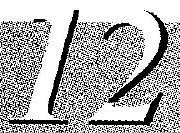
\includegraphics[max width=\textwidth, center]{2024_10_30_26b590fd1106d28139f0g-074}

\section*{分式方程}
城上青山如屋里,东家流水入西邻。

王维《春日与裴迪过新昌里访昌逸人不遇》

分母中含有未知数的方程,叫做分式方程。\\
解分式方程的基本思路是,"东家"分式化为"西邻"整式,将分式方程化为整式方程来求解。通常利用去分母、换元以及基本的恒等变形等手段来转化方程。当然,在转化的过程中,需注意未知数的取值范围的变化,因为这有可能引起增根。

例1 解方程 $\frac{5-2 x}{2 x-3}=\frac{4-3 x}{3 x-2}$ 。\\
基本思路 或直接去分母;或在方程两边加 1 ;或将分式简化为分子是常数的分式与某常数之和,简便求解,但需验根。

解法 1 去分母,得

\begin{align*}
\begin{aligned}
(5-2 x)(3 x-2) & =(4-3 x)(2 x-3) \\
15 x-6 x^{2}-10+4 x & =8 x-6 x^{2}-12+9 x
\end{aligned}
\end{align*}

解得

\begin{align*}
x=-1
\end{align*}

经验根知 $x=-1$ 为原方程的解。\\
解法2 方程两边加 1 ,得

即

\begin{align*}
\frac{5-2 x}{2 x-3}+1=\frac{4-3 x}{3 x-2}+1
\end{align*}

\begin{align*}
\begin{aligned}
& \frac{2}{2 x-3}=\frac{2}{3 x-2} \\
& 2 x-3=3 x-2
\end{aligned}
\end{align*}

业务:初高中联赛班、培优班、美国高中数学、教师培训、机构教学产品研发、讲义资料出售等\\
解得

\begin{align*}
x=-1
\end{align*}

验根知 $x=-1$ 为原方程的解。\\
解法 3 原式可化为 $\frac{2}{2 x-3}-1=\frac{2}{3 x-2}-1$ ,\\
所以

\begin{align*}
\frac{2}{2 x-3}=\frac{2}{3 x-2}
\end{align*}

以下同解法 2 。\\
例2 解方程 $|x|-\frac{4}{x}=\frac{3|x|}{x}$ 。\\
基本思路 分 $x>0$ 与 $x<0$ 情形转化分式方程为一元二次方程 $x^{2}-$ $3 x-4=0(x>0)$ 或 $x^{2}-3 x+4=0(x<0)$.

解 由题意得 $x \neq 0$ 。\\
当 $x>0$ 时, 原方程化为

\begin{align*}
x-\frac{4}{x}=3
\end{align*}

两边同乘 $x$ 并整理得

\begin{align*}
\begin{aligned}
& x^{2}-3 x-4=0, \\
& x=4 \text { 或 } x=-1 .
\end{aligned}
\end{align*}

因 $x>0$ ,则 $x=-1$ 不合题意,舍去。\\
当 $x<0$ 时, 原方程化为

\begin{align*}
-x-\frac{4}{x}=-3
\end{align*}

两边同乘 $x$ 并整理得

\begin{align*}
x^{2}-3 x+4=0
\end{align*}

因为 $\Delta=(-3)^{2}-4 \times 4=-7<0$ ,所以方程 $x^{2}-3 x+4=0$ 无解。故原方程的解为 $x=4$ 。\\
例3 解方程

\begin{align*}
\frac{x+6}{x+1}-\frac{3 x^{2}+10 x+4}{x^{2}+3 x+2}+\frac{2 x+1}{x+2}=0
\end{align*}

基本思路 观察方程先简化方程左边的三个分式,之后通分 $(x+1)(x+$ 2),原方程可化为 $x+9=0$ 。

解 观察方程知,原方程可以转化为

\begin{align*}
1+\frac{5}{x+1}-\left(3+\frac{x-2}{x^{2}+3 x+2}\right)+2-\frac{3}{x+2}=0
\end{align*}

业务:初高中联赛班、培优班、美国高中数学、教师培训、机构教学产品研发、讲义资料出售等整理得

\begin{align*}
\frac{5}{x+1}-\frac{x-2}{x^{2}+3 x+2}-\frac{3}{x+2}=0
\end{align*}

去分母,整理得

\begin{align*}
x+9=0, x=-9
\end{align*}

经检验知, $x=-9$ 是原方程的解。\\
例4 解方程 $\frac{1}{x^{2}+x-2}+\frac{1}{x^{2}+7 x+10}=2$ 。\\
基本思路 $\quad$ 利用 $\frac{1}{x^{2}+x-2}=\frac{1}{3}\left(\frac{1}{x-1}-\frac{1}{x+2}\right)$ 和 $\frac{1}{x^{2}+7 x+10}=$ $\frac{1}{3}\left(\frac{1}{x+2}-\frac{1}{x+5}\right)$ ,化简方程为 $x^{2}+4 x-6=0$ 。

解 原方程变形为

得

\begin{align*}
\begin{gathered}
\frac{1}{(x+2)(x-1)}+\frac{1}{(x+2)(x+5)}=2, \\
\frac{1}{3}\left(\frac{1}{x-1}-\frac{1}{x+2}\right)+\frac{1}{3}\left(\frac{1}{x+2}-\frac{1}{x+5}\right)=2, \\
\frac{1}{x-1}-\frac{1}{x+5}=6,
\end{gathered}
\end{align*}

两边同乘以 $(x-1)(x+5)$ ,并整理得

\begin{align*}
x+5-(x-1)=6(x-1)(x+5)
\end{align*}

即

\begin{align*}
x^{2}+4 x-6=0,
\end{align*}

解得

\begin{align*}
x_{1}=-2-\sqrt{10}, x_{2}=-2+\sqrt{10}
\end{align*}

经检验,原方程的两根为 $x_{1}=-2-\sqrt{10}, x_{2}=-2+\sqrt{10}$ 。\\
思考(1)本题还有其他解法吗?\\
(2) 对于多项和的分式方程,如果每个分式具有共同特征 $\frac{1}{(x+a)(x+b)}=$ $\frac{1}{a-b}\left(\frac{1}{x+b}-\frac{1}{x+a}\right)$ ,那么就可以利用此特征简捷地转化方程。如解方程 $\frac{1}{x(x-1)}+\frac{1}{x(x+1)}+\cdots+\frac{1}{(x+9)(x+10)}=\frac{11}{12}$.

读者可自行尝试解此方程.

例 5 解方程组

\begin{align*}
\left\{\begin{array}{l}
\frac{10}{x+y}+\frac{3}{x-y}=-5 \\
\frac{15}{x+y}-\frac{2}{x-y}=-1
\end{array}\right.
\end{align*}

基本思路 观察方程特点,可用换元法,令 $\frac{1}{x+y}=u, \frac{1}{x-y}=v$ ,转化方程组为二元一次方程组,解出 $u, v$ ,再回代解关于 $x, y$ 的二元一次方程组。还可以直接通分转化为(参见第14讲)二元二次方程组。

解 令 $\frac{1}{x+y}=u, \frac{1}{x-y}=v$ ,原方程组可化为

\begin{align*}
\left\{\begin{array}{l}
10 u+3 v=-5 \\
15 u-2 v=-1
\end{array}\right.
\end{align*}

解这个方程组,得

\begin{align*}
\left\{\begin{array} { l } 
{ u = - \frac { 1 } { 5 } , } \\
{ v = - 1 , }
\end{array} \text { 即 } \left\{\begin{array}{l}
x+y=-5, \\
x-y=-1 .
\end{array}\right.\right.
\end{align*}

解之得

\begin{align*}
\left\{\begin{array}{l}
x=-3 \\
y=-2
\end{array}\right.
\end{align*}

经检验 $\left\{\begin{array}{l}x=-3, \\ y=-2\end{array}\right.$ 是原方程组的解。\\
例6 某商场在一楼和二楼之间安装了一部自动扶梯,以均匀的速度向上行驶,一男孩和一女孩同时从自动扶梯上走到二楼(扶梯行驶,两人也走梯),如果两人上梯的速度都是匀速的,每次只跨 1 级,且男孩每分钟走动的级数是女孩的两倍。已知男孩走了 27 级到达扶梯顶部,而女孩走了 18 级到达顶部。问扶梯露在外面的部分有多少级?

基本思路 大胆设元,设女孩、自动扶梯速度分别为 $x$ 级/分, $y$ 级/分,扶梯露在外面部分为 $s$ 级,列出方程组。

解 设女孩上梯的速度为 $x$ 级/分,自动扶梯的速度为 $y$ 级/分,扶梯露在外面的部分有 $s$ 级,则男孩上梯的速度为 $2 x$ 级/分,且有

\begin{align*}
\left\{\begin{array}{l}
\frac{27}{2 x}=\frac{s-27}{y} \\
\frac{18}{x}=\frac{s-18}{y}
\end{array}\right.
\end{align*}

业务:初高中联赛班、培优班、美国高中数学、教师培训、机构教学产品研发、讲义资料出售等两个方程两边分别相除,得

\begin{align*}
\begin{gathered}
\frac{27}{36}=\frac{s-27}{s-18} \\
s=54
\end{gathered}
\end{align*}

所以扶梯露在外面的部分有 54 级。\\
例7 若实数 $x, y, z$ 满足 $x+\frac{1}{y}=4, y+\frac{1}{z}=1, z+\frac{1}{x}=\frac{7}{3}$, 求 $x y z$的值。

基本思路 题中有三个元 $x, y, z$ ,可先化为关于一个元如 $x$ 的关系式,进而转化为 $x$ 的一元二次方程。

解 因为

\begin{align*}
\begin{aligned}
4 & =x+\frac{1}{y}=x+\frac{1}{1-\frac{1}{z}}=x+\frac{z}{z-1} \\
& =x+\frac{\frac{7}{3}-\frac{1}{x}}{\frac{7}{3}-\frac{1}{x}-1} \\
& =x+\frac{7 x-3}{4 x-3}
\end{aligned}
\end{align*}

则有

\begin{align*}
4(4 x-3)=x(4 x-3)+7 x-3
\end{align*}

即

\begin{align*}
(2 x-3)^{2}=0
\end{align*}

得

\begin{align*}
x=\frac{3}{2} .
\end{align*}

所以

\begin{align*}
z=\frac{7}{3}-\frac{1}{x}=\frac{5}{3}, y=1-\frac{1}{z}=\frac{2}{5} .
\end{align*}

于是 $x y z=1$.\\
思考 如果 $x+\frac{1}{y}=y+\frac{1}{z}=z+\frac{1}{x}, x, y, z$ 是实数,问 $x y z$ 的值是多少?\\
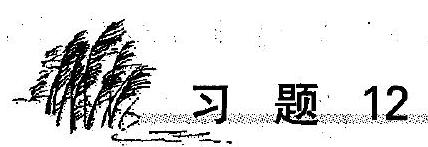
\includegraphics[max width=\textwidth, center]{2024_10_30_26b590fd1106d28139f0g-078}

ㅣ 解方程 $\frac{x+1}{x+2}+\frac{x+6}{x+7}=\frac{x+2}{x+3}+\frac{x+5}{x+6}$.

23 解方程 $\frac{4 x}{x^{3}+2 x^{2}+x}+\frac{5 x}{x^{3}+2 x^{2}-5 x}+\frac{3}{2}=0$.\\
3 解关 $x$ 方程 $x+\frac{1}{x}=a+\frac{1}{a}$ ( $a$ 是实数).\\
蛙若关于 $x$ 的方程 $\left|\frac{x^{2}}{x-1}\right|=a$ 仅有两个不同的实根,则实数 $a$ 的取值范围是().(2006 年全国初中数学联赛题)\\
(A) $a>0$\\
(B) $a \geqslant 4$\\
(C) $2<a<4$\\
(D) $0<a<4$

5 解方程 $\frac{x^{2}+x+1}{x^{2}+1}+\frac{2 x^{2}+x+2}{x^{2}+x+1}=\frac{19}{6}$.\\
6解方程 $\frac{2 x^{2}+3 x+2}{2 x^{2}-3 x-2}=\frac{2 x^{2}-5 x+3}{2 x^{2}+5 x-3}$.\\
7 解方程 $\frac{1}{x^{2}+11 x-8}+\frac{1}{x^{2}+2 x-8}+\frac{1}{x^{2}-13 x-8}=0$.\\
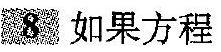
\includegraphics[max width=\textwidth, center]{2024_10_30_26b590fd1106d28139f0g-079}

\begin{align*}
\frac{x}{x-2}+\frac{x-2}{x}+\frac{2 x+a}{x(x-2)}=0
\end{align*}

只有一个实数解,求 $a$ 的值及对应的原方程的解。\\
97 有一列火车于上午7:45 从甲地出发开往乙地,另一列火车于上午8:15由乙地开往甲地。第一列火车在两列火车中途相遇后 40 分钟抵达乙地,而第二列火车在两列火车中途相遇后 1 小时 40 分抵达甲地。假设两列火车都以匀速行驶(但两者速度不必相同),请问此两列火车何时相遇?\\
篓10汽艇与木筏同时离开码头 $A$ 顺水出发,汽艇顺水航行 96 千米,掉头返回 A处点需 14 小时,若已知汽艇在返回途中离码头 A 24 干米处与木筏相遇,求汽艇在静水中的速度与在顺水中的速度。

\section*{L鳘体操}
清末大文豪俞曲园先生曾写过一首脍多人口的诗:\\
重重叠叠山,曲曲环环路,\\
叮叮咚咚泉,高高下下树。

全国小学奥数群:221739457,全国初中奥数学生群:253736211,全国高中奥数学生群591782992全国初中奥数教练群112464128,全国高中奥数教练群195949359\\
竞赛公众号:新浪微博@郑剑雄 微信:v136257437 QQ:136257437\\
业务:初高中联赛班、培优班、美国高中数学、教师培训、机构教学产品研发、讲义资料出售等有趣的是,我们可以把它改写成下面的加法坚式,诗句与算式相对应,这恐怕连当年的俞曲园先生也没有料想到吧?

\begin{center}
\begin{tabular}{|c|c|c|}
\hline
\multicolumn{3}{|r|}{重 曲} \\
\hline
十重 叠 & 十曲 & 环 \\
\hline
叠 山 & 环 & 路 \\
\hline
叮 &  & 高 \\
\hline
十可 咚 & 十高 & 下 \\
\hline
咚 泉 & 下 & 树 \\
\hline
\end{tabular}
\end{center}

可以看出,这四个加法算式,都可以用一个字母竖式来表示,即

\begin{center}
\begin{tabular}{r}
$A$ \\
$+A \quad B$ \\
\hline
$B \quad C$ \\
\hline
\end{tabular}
\end{center}

那么满足条件的算式有哪些呢?\\
经过计算,这个算式正好有四个解。请你试着解出答案.

\section*{夏门郑剑雄高中数学竞赛系列}
全国小学奥数群:221739457,全国初中奥数学生群:253736211,全国高中奥数学生群591782992全国初中奥数教练群112464128,全国高中奥数教练群195949359竞赛公众号:新浪微博@郑剑雄 微信:v136257437 QQ:136257437业务:初高中联赛班、培优班、美国高中数学、教师培训、机构教学产品研发、讲义资类售等\\
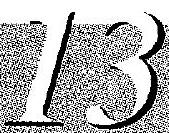
\includegraphics[max width=\textwidth, center]{2024_10_30_26b590fd1106d28139f0g-081}

\section*{无理方程}
东边日出西边雨,道是无晴却有晴。

刘禹锡《竹枝词一首(其一)》

根号内含有未知数的方程,叫做无理方程。\\
解无理方程的基本思路,就是"无理"却"有理",把它化为有理方程。通常利用配方、换元、因式分解等方式转化方程。

在处理无理方程时,需注意可能出现的增根。\\
例1 解方程 $2 x^{2}-15 x-\sqrt{2 x^{2}-15 x+1998}=-18$.\\
基本思路 观察方程的特点,整体换元 $\sqrt{2 x^{2}-15 x+1998}=y$ ,转化为方程 $y^{2}-y-1980=0$, 然后, 求解方程 $2 x^{2}-15 x-27=0$ 。

解 由题意得 $2 x^{2}-15 x+1998 \geqslant 0$.\\
令 $y=\sqrt{2 x^{2}-15 x+1998}$, 则 $y \geqslant 0$, 且原方程化为

\begin{align*}
y^{2}-y-1980=0
\end{align*}

解得

\begin{align*}
y_{1}=45, y_{2}=-44
\end{align*}

但 $y \geqslant 0$ ,所以 $y_{2}=-44$ 不合题意,舍去。

于是有\\
两边平方整理得

解得

\begin{align*}
\sqrt{2 x^{2}-15 x+1998}=45
\end{align*}

\begin{align*}
2 x^{2}-15 x-27=0
\end{align*}

\begin{align*}
x_{1}=9, x_{2}=-\frac{3}{2} .
\end{align*}

由 $x_{1}=9, x_{2}=-\frac{3}{2}$ 都使得 (1) 式成立, 可知原方程的解为

业务:初高中联赛班、培优班、美国高中数学、教师培训、机构教学产品研发、讲义资料出售等

\begin{align*}
x_{1}=9, x_{2}=-\frac{3}{2} .
\end{align*}

例 2 设实数 $x>0$ ,求使等式

\begin{align*}
\sqrt{x^{2}-1}+\sqrt{x^{2}+4 x+3}=\sqrt{3 x^{2}+4 x+1}
\end{align*}

成立的所有 $x$ 的值.\\
基本思路 观察等式即知方程的各项中都有式子 $\sqrt{x+1}$ (因为 $x>0$ ,得 $x+1>0$ ),从而转化原方程为 $\sqrt{x+1}=0$ 和 $\sqrt{x-1}+\sqrt{x+3}=\sqrt{3 x+1}$ 。然后,逐步去根号转化为易求解的方程。

解 $\sqrt{(x+1)(x-1)}+\sqrt{(x+1)(x+3)}=\sqrt{(3 x+1)(x+1)}$.\\
因为 $x>0$, 所以 $x+1>0$, 从而知 $x-1 \geqslant 0, x+3>0,3 x+1>0$,于是有 $\sqrt{x+1}=0$ 或 $\sqrt{x-1}+\sqrt{x+3}=\sqrt{3 x+1}$ 。

由 $\sqrt{x+1}=0$ 得 $x_{1}=-1$.\\
由 $\sqrt{x-1}+\sqrt{x+3}=\sqrt{3 x+1}$ ,两边平方整理得

\begin{align*}
2 \sqrt{(x-1)(x+3)}=x-1
\end{align*}

从而有 $\sqrt{x-1}=0$ 或 $2 \sqrt{x+3}=\sqrt{x-1}$, 于是 $\sqrt{x-1}=0$ 得 $x_{2}=1$,由 $2 \sqrt{x+3}=\sqrt{x-1}$ 得 $x_{3}=-\frac{13}{3}$.

经检验, $x=1$ 为符合题中要求的 $x$ 。\\
说明 还可以直接通过平方逐次去根号转化为多项式方程求解. 若用此方法,则题中条件 $x>0$ 可去掉。

例3 解方程 $x^{5}-33 x^{2} \sqrt{x}+32=0$ 。\\
基本思路 观察到 $x^{2} \sqrt{x}=x^{\frac{5}{2}}$ 与 $x^{5}$ 之间的平方关系,转化方程为 $y^{2}-$ $33 y+32=0$, 这里 $y=x^{\frac{5}{2}}$ 。

解 考虑到 $x^{2} \sqrt{x}=x^{\frac{5}{2}}$ ,则可令 $x^{\frac{5}{2}}=y$ ,原方程可化为

\begin{align*}
y^{2}-33 y+32=0
\end{align*}

解得

\begin{align*}
y_{1}=1, y_{2}=32 .
\end{align*}

于是 $x^{\frac{5}{2}}=1$ 或 $x^{\frac{5}{2}}=32$ ,得 $x_{1}=1, x_{2}=4$ 。\\
说明 用换元法常能简化问题。\\
例 4 解方程

\begin{align*}
\sqrt{x+3-4 \sqrt{x-1}}+\sqrt{x+8-6 \sqrt{x-1}}=1
\end{align*}

基本思路 看似复杂,实质简单,两个大根号下均为形如 $(a-b)^{2}$ ,从而简化方程为 $|\sqrt{x-1}-2|+|\sqrt{x-1}-3|=1$ 。

解 考虑到 $x+3-4 \sqrt{x-1}=(x-1)-4 \sqrt{x-1}+4=(\sqrt{x-1}-$ $2)^{2}, x+8-6 \sqrt{x-1}=(x-1)-6 \sqrt{x-1}+9=(\sqrt{x-1}-3)^{2}$, 则原方程化为

即

\begin{align*}
\sqrt{(\sqrt{x-1}-2)^{2}}+\sqrt{(\sqrt{x-1}-3)^{2}}=1
\end{align*}

\begin{align*}
|\sqrt{x-1}-2|+|\sqrt{x-1}-3|=1
\end{align*}

(1)当 $\sqrt{x-1}<2$ 时,原方程变形为

\begin{align*}
2-\sqrt{x-1}+3-\sqrt{x-1}=1
\end{align*}

解得 $\sqrt{x-1}=2$ ,这与 $\sqrt{x-1}<2$ 矛盾,无解。\\
(2) 当 $2 \leqslant \sqrt{x-1}<3$ 时,原方程变形为

\begin{align*}
\sqrt{x-1}-2+3-\sqrt{x-1}=1
\end{align*}

即当 $2 \leqslant \sqrt{x-1}<3$ 时的一切 $x$ 都是方程的解,解得 $5 \leqslant x<10$ 。\\
(3)当 $\sqrt{x-1} \geqslant 3$ 时,原方程变形为

\begin{align*}
\sqrt{x-1}-2+\sqrt{x-1}-3=1
\end{align*}

解得

\begin{align*}
x=10
\end{align*}

综上所述,方程的解为 $5 \leqslant x \leqslant 10$ 。\\
经检验, $5 \leqslant x \leqslant 10$ 是原方程的解。\\
例 5 已知 $a \geqslant 2$ ,求方程 $\sqrt{a-\sqrt{a+x}}=x$ 的所有实根之和。\\
基本思路 引人另一个元 $y=\sqrt{a+x}$ ,以 $x, y$ 形式构成等式 $y^{2}-x-$ $y=x^{2}$ ,简化为 $x+y=0$ 或 $x-y=-1$ 。然后,求解方程 $x+1=\sqrt{a+x}$ 。

解 由题意得 $x \geqslant 0$, 又 $a \geqslant 2$, 则 $a+x>0, a \geqslant \sqrt{a+x}$, 且 $a-\sqrt{a+x}=$ $x^{2}$,

令 $\sqrt{a+x}=y$, 则 $a \geqslant y>0$, 且 $a-y=x^{2}$ 。\\
又 $y^{2}=a+x$ ,于是

得

\begin{align*}
\begin{gathered}
y^{2}-x-y=x^{2} \\
-(x+y)=(x-y)(x+y)
\end{gathered}
\end{align*}

业务:初高中联赛班、培优班、美国高中数学、教师培训、机构教学产品研发、讲义资料出售等\\
而 $x+y>0$, 所以 $x-y=-1$, 即 $x-\sqrt{a+x}=-1$, 整理得

两边平方得

解得

\begin{align*}
\begin{gathered}
x+1=\sqrt{a+x} \\
x^{2}+x+1-a=0 \\
x_{1,2}=\frac{-1 \pm \sqrt{4 a-3}}{2}
\end{gathered}
\end{align*}

又 $x \geqslant 0$, 所以满足要求的实数根为 $x=\frac{-1+\sqrt{4 a-3}}{2}$.\\
故原方程的实根之和为 $x=\frac{-1+\sqrt{4 a-3}}{2}$ 。\\
思考 你还能有其他解法吗?

\section*{习 题 13}
1 已知 $\left(x+\sqrt{x^{2}+2002}\right)\left(y+\sqrt{y^{2}+2002}\right)=2002$, 求 $x^{2}-3 x y-4 y^{2}-$ $6 x-6 y+58$ 的值.

2 若关于 $x$ 的方程 $a \sqrt{x^{2}}+\frac{1}{2} \sqrt[4]{x^{2}}-\frac{1}{3}=0$ 恰有两个不同的实数解,求实数 $a$ 的取值范围。\\
3 解方程 $4 x^{2}+2 x \sqrt{3 x^{2}+x}+x-9=0$ 。\\
4 解方程 $5 \sqrt{x}+5 \sqrt{2 x+3}+2 \sqrt{2 x^{2}+3 x}=11-3 x$.\\
5 解方程 $x^{2}-6 x-6+x \sqrt{x^{2}-2 x-2}=0$.\\
6 解方程 $\sqrt[3]{2+x}=1-\sqrt{x+1}$.\\
7 解方程 $\sqrt{x^{2}+9}+\sqrt{x^{2}-9}=\sqrt{7}+5$.\\
8 解方程 $\sqrt{\sqrt{3}-\sqrt{\sqrt{3}+x}}=x$.

\section*{心智体操}
\section*{相信自己,发挥僣能}
在动物园里的小骆驼问妈妈:"为什么我们的睫毛那么长?"骆驼妈妈说: "当风沙来的时候,长长的睫毛可以让我们挡住风沙看清方向。"

小骆驼又问:"为什么我们的背那么驼?"骆驼妈妈说:"这个叫驼峰,可以帮我们储存大量的水和养分,让我们能在沙漠里耐受十几天无水无食的日子。"

小骆驼又问:"为什么我们的脚掌那么厚?"骆驼妈妈说:"那可以让我们重重的身子不至于陷在软软的沙子里,便于长途跋涉呀。"小骆驼高兴极了: "哇,原来我们这么有用啊!可是为什么我们还在动物园里,不去沙漠远足呢?"

望夫处,江悠悠\\
化为石,不回头:\\
山头日日风复雨,行人归来石应语。

\section*{王建《望夫石》}
解二元二次方程组的基本思路就是转化,"不回头",即"消元"、"降次".通过直接代入、因式分解、配方、换元等手段达到消元、降次的目的。

有时,将所解方程组转化为基本方程组 $\left\{\begin{array}{l}x+y=a , \\ x y=b ,\end{array}\right.$ 特别是由二元对称方程(方程中未知数 $x, y$ 互换后方程保持不变的二元方程)组成的方程组,其基本解题思路之一就是化方程组为上述基本方程组。

有时,还会将二元二次方程,视其为关于一个未知数的含字母的一元二次方程,利用一元二次方程的根的判别式及其他基本知识来"各个击破",达到求解二元二次方程组的目的。

例1 已知方程组

\begin{align*}
\left\{\begin{array}{l}
y=a x^{2}+b x+c \\
y=k(x-1)-\frac{k^{2}}{4}
\end{array}\right.
\end{align*}

对于任意的实数 $k$ 都只有一组实数解,求 $a, b, c$.\\
基本思路 消去 $y$ 转化为关于 $x$ 的方程 $a x^{2}+(b-k) x+\left(c+k+\frac{k^{2}}{4}\right)=$ 0 ,由判别式 $\Delta=0$ 及 $k$ 的任意性得关于 $a, b, c$ 的方程组。

解 由题意得

\begin{align*}
a x^{2}+b x+c=k(x-1)-\frac{k^{2}}{4}
\end{align*}

整理得

\begin{align*}
a x^{2}+(b-k) x+\left(c+k+\frac{k^{2}}{4}\right)=0
\end{align*}

\begin{align*}
\begin{aligned}
& \text { 又 } \Delta=(b-k)^{2}-4 a\left(c+k+\frac{k^{2}}{4}\right)=0 \text {, 即 } \\
&(1-a) k^{2}-2(b+2 a) k+\left(b^{2}-4 a c\right)=0 .
\end{aligned}
\end{align*}

由于上式对于任意的实数 $k$ 都成立,因此有

\begin{align*}
1-a=0, b+2 a=0, b^{2}-4 a c=0,
\end{align*}

解得

\begin{align*}
a=1, b=-2, c=1
\end{align*}

于是有

\begin{align*}
a=1, b=-2, c=1
\end{align*}

例2 解方程组

\begin{align*}
\left\{\begin{array}{l}
x^{2}-5 x-y^{2}-5 y=0 \\
x^{2}+x y+y^{2}=49
\end{array}\right.
\end{align*}

基本思路 先看方程 $x^{2}-5 x-y^{2}-5 y=0$ ,可考虑因式分解降次,得方程 $x+y=0$ 或 $x-y-5=0$ ,从而将原方程组转化为一个二元一次方程与一个二元二次方程组成的方程组,用代人消元法易于求解。

解 因为 $x^{2}-5 x-y^{2}-5 y=\left(x^{2}-y^{2}\right)-5(x+y)$

\begin{align*}
\begin{aligned}
& =(x-y)(x+y)-5(x+y) \\
& =(x+y)(x-y-5)
\end{aligned}
\end{align*}

所以

\begin{align*}
x^{2}-5 x-y^{2}-5 y=(x+y)(x-y-5)=0
\end{align*}

即有

\begin{align*}
x+y=0 \text { 或 } x-y-5=0 .
\end{align*}

于是方程组化为

\begin{align*}
\left\{\begin{array} { l } 
{ x + y = 0 , } \\
{ x ^ { 2 } + x y + y ^ { 2 } = 4 9 }
\end{array} \text { 或 } \left\{\begin{array}{l}
x-y-5=0, \\
x^{2}+x y+y^{2}=49 .
\end{array}\right.\right.
\end{align*}

用代入消元法,解得原方程组的解为

\begin{align*}
\left\{\begin{array} { l } 
{ x _ { 1 } = - 7 , } \\
{ y _ { 1 } = 7 ; }
\end{array} \left\{\begin{array} { l } 
{ x _ { 2 } = 7 , } \\
{ y _ { 2 } = - 7 ; }
\end{array} \left\{\begin{array} { l } 
{ x _ { 3 } = \frac { 5 + \sqrt { 5 7 } } { 2 } , } \\
{ y _ { 3 } = \frac { - 5 + \sqrt { 5 7 } } { 2 } ; }
\end{array} \left\{\begin{array}{l}
x_{4}=\frac{5-\sqrt{57}}{2} \\
y_{4}=\frac{-5-\sqrt{57}}{2}
\end{array}\right.\right.\right.\right.
\end{align*}

说明 通过因式分解转化题中方程组为容易解的方程组,这是解二元二次方程组的基本思路之一。

业务:初高中联赛班、培优班、美国高中数学、教师培训、机构教学产品研发、讲义资料出售等\\
例3 解方程组

\begin{align*}
\left\{\begin{array}{l}
(x+y)^{2}-2 x y-x^{2} y^{2}=10 \\
x+y-x y=4
\end{array}\right.
\end{align*}

基本思路 观察方程组的特征,发现虽不可用因式分解的方法来降次,但是,可以根据题中 $x+y, x y$ 的特征,考虑整体变换,令 $x+y=u, x y=v$ ,转化方程组为

\begin{align*}
\left\{\begin{array}{l}
u^{2}-2 v-v^{2}=10 \\
u-v=4
\end{array}\right.
\end{align*}

代入消元解得 $u$ 与 $v$ ,从而求得 $x$ 与 $y$ 。\\
解 令 $x+y=u, x y=v$, 则原方程组可转化为

\begin{align*}
\left\{\begin{array}{l}
u^{2}-2 v-v^{2}=10 \\
u-v=4
\end{array}\right.
\end{align*}

所以把 $u=4+v$ 代入上述方程组的第一个方程中, 得

解得

\begin{align*}
\begin{gathered}
(4+v)^{2}-2 v-v^{2}=10, \\
v=-1, \text { 从而 } u=3 .
\end{gathered}
\end{align*}

于是得

\begin{align*}
\left\{\begin{array}{l}
x+y=3 \\
x y=-1
\end{array}\right.
\end{align*}

即 $x, y$ 是方程 $z^{2}-3 z-1=0$ 的两个根,解此方程得两个根是 $\frac{3 \pm \sqrt{13}}{2}$.\\
因此,原方程组的解是

说明 对于含有对称式 $x+y, x y, x^{2}+y^{2}$ 等二元二次方程组,可以考虑\\

\includegraphics[max width=\textwidth, center]{2024_10_30_26b590fd1106d28139f0g-088}

例 4 解方程组

\begin{align*}
\left\{\begin{array}{l}
x+y=2  \tag{1}\\
x y-z^{2}=1
\end{array}\right.
\end{align*}

物理竞赛群:271751860,化学竞赛群:271751511,生物竞赛群:254139830,信息竞赛群:281798334,英语竞赛群:271750414,英语 $\square$ 语群:168570356,心算交流群:131033273,厦门培训机构教师招聘

基本思路 用代入法解,或将 $x$ 与 $y$ 看作是一个一元二次方程 $t^{2}-2 t+$ $z^{2}+1=0$ 的两根,由判别式 $\Delta \geqslant 0$ ,得 $z=0$ 。

解法 1 由(1), 得\\
把(3)代入(2),得\\
即\\
配方,得\\
所以

\begin{align*}
y=2-x \tag{3}
\end{align*}

\begin{align*}
2 x-x^{2}-z^{2}=1
\end{align*}

\begin{align*}
x^{2}-2 x+1+z^{2}=0
\end{align*}

\begin{align*}
(x-1)^{2}+z^{2}=0
\end{align*}

\begin{align*}
x=1, z=0
\end{align*}

把 $x=1$ 代入 (3), 得 $y=1$ 。\\
故原方程组的解为 $\left\{\begin{array}{l}x=1, \\ y=1, \\ z=0 .\end{array}\right.$\\
解法2 由(2)得 $x y=z^{2}+1$ 。\\
由(1)、(4)知 $x, y$ 是关于 $t$ 的一元二次方程

\begin{align*}
t^{2}-2 t+z^{2}+1=0
\end{align*}

的两根,而此方程的判别式

\begin{align*}
\Delta=4-4\left(z^{2}+1\right)=-4 z^{2} \geqslant 0
\end{align*}

即

\begin{align*}
z^{2} \leqslant 0
\end{align*}

但 $z^{2} \geqslant 0$ ,所以 $z^{2}=0, z=0$ 。\\
此时,关于 $t$ 的一元二次方程为 $t^{2}-2 t+1=0$ ,有两等根1,所以 $x=$ $y=1$ ,从而得原方程组的解为

\begin{align*}
\left\{\begin{array}{l}
x=1 \\
y=1 \\
z=0
\end{array}\right.
\end{align*}

说明 还可以考虑代换 $x=s+t, y=s-t$, 有 $x+y=2 s=2, s=1$,即 $x=1+t, y=1-t$ ,把它们代人方程(2),得 $1-t^{2}-z^{2}=1$ ,所以 $t^{2}+$ $z^{2}=0$, 得 $t=0, z=0$. 从而 $x=1+t=1, y=1-t=1$ 。

例5 已知正实数 $a, b$ 满足方程组 $\left\{\begin{array}{l}a+b^{2}+a b=31, \\ b+a^{2}+a b=25,\end{array}\right.$ 则 $a+b$ 的值是\\
$\qquad$。(2011 年"时代杯"江苏省中学数学应用与创新邀请赛题)\\
基本思路 乍看需求解二元二次方程组,但细看,可相加两个等式转化

业务:初高中联赛班、培优班、美国高中数学、教师培训、机构教学产品研发、讲义资料出售等为形如 $u^{2}+u-56=0$ ,而求得 $u(=a+b)$ 的结果。

解 二式相加,得 $(a+b)+\left(a^{2}+b^{2}+2 a b\right)=56$ ,则有

\begin{align*}
(a+b)^{2}+(a+b)-56=0
\end{align*}

因式分解得 $[(a+b)+8][(a+b)-7]=0$.\\
因为 $a, b$ 都是正实数, 所以 $a+b+8>0$, 从而 $a+b-7=0$ 。\\
故 $a+b=7$ 。\\
说明 若题目改为三个正实数 $a, b, c$ ,满足方程组

\begin{align*}
\left\{\begin{array}{l}
a+b^{2}+2 a b=9 \\
b+c^{2}+2 b c=47 \\
c+a^{2}+2 a c=16
\end{array}\right.
\end{align*}

你能求得 $a+b+c$ 的值吗?\\
例 6 在直角三角形 $A B C$ 中, $a, b, c$ 表示各边的长, 其中 $c$ 为斜边. 若 $\frac{b}{c-a}+\frac{a}{c-b}=6 \frac{1}{2}$, 则 $a: b: c=$ $\qquad$ .

基本思路 换元 $\frac{a}{c}=x, \frac{b}{c}=y$ 得方程组 $x^{2}+y^{2}=1$ 及 $\frac{y}{1-x}+$ $\frac{x}{1-y}=\frac{13}{2}$, 然后仿照例 3 的思路求出 $x$ 与 $y$.

解 令 $x=\frac{a}{c}, y=\frac{b}{c}$ ,则由 $a^{2}+b^{2}=c^{2}$ ,得

\begin{align*}
x^{2}+y^{2}=1 \tag{1}
\end{align*}

由 $\frac{b}{c-a}+\frac{a}{c-b}=6 \frac{1}{2}$ 得 $\frac{y}{1-x}+\frac{x}{1-y}=\frac{13}{2}$, 即

\begin{align*}
13 x y=15(x+y)-15 \tag{2}
\end{align*}

再令 $x+y=u, x y=v$ ,将方程组化为

\begin{align*}
\left\{\begin{array}{l}
u^{2}-2 v=1 \\
13 v=15 u-15
\end{array}\right.
\end{align*}

解得 $\left\{\begin{array}{l}u=\frac{17}{13}, \\ v=\frac{60}{13^{2}} .\end{array}\right.$ (负值 $u$ 已舍去), 即 $\left\{\begin{array}{l}x+y=\frac{17}{13}, \\ x y=\frac{60}{169} .\end{array}\right.$\\

\includegraphics[max width=\textwidth, center]{2024_10_30_26b590fd1106d28139f0g-090}

业务:初高中联赛班、培优班、美国高中数学、教师培训、机构教学产品研发、讲义资料出售等\\
于是 $x, y$ 为方程 $t^{2}-\frac{17}{13} t+\frac{60}{169}=0$ 的两根,解得 $\left\{\begin{array}{l}x=\frac{5}{13}, \\ y=\frac{12}{13} ;\end{array}\right.$ 或 $\left\{\begin{array}{l}x=\frac{12}{13}, \\ y=\frac{5}{13} .\end{array}\right.$\\
故 $a: b: c=x: y: 1$, 从而得 $a: b: c=12: 5: 13$, 或 $a: b: c=5:$ 12 : 13.

例7 解方程组 $\left\{\begin{array}{l}\frac{1}{x}+\frac{1}{y+z}=\frac{1}{2}, \\ \frac{1}{y}+\frac{1}{z+x}=\frac{1}{3}, \\ \frac{1}{z}+\frac{1}{x+y}=\frac{1}{4} .\end{array}\right.$\\
解 由方程组可知

\begin{align*}
x \neq 0, y \neq 0, z \neq 0, y+z \neq 0, x+z \neq 0, x+y \neq 0, \tag{1}
\end{align*}

于是原方程组变形为

\begin{align*}
\left\{\begin{array}{l}
2(x+y+z)=x(y+z)  \tag{2}\\
3(x+y+z)=y(z+x) \\
4(x+y+z)=z(x+y)
\end{array}\right.
\end{align*}

若 $x+y+z=0$, 则 $x=0$ 或 $y+z=0$ ,这与 (1) 矛盾.\\
所以 $x+y+z \neq 0$ ,从而把 (2)、(3)、(4) 变形为

\begin{align*}
\frac{x(y+z)}{2}=\frac{y(z+x)}{3}=\frac{z(x+y)}{4}=x+y+z=k \neq 0 .
\end{align*}

故方程组转化为

得

\begin{align*}
\begin{gather*}
\left\{\begin{array}{l}
x y+x z=2 k, \\
y z+x y=3 k, \\
z x+z y=4 k,
\end{array}\right. \\
\left\{\begin{array}{l}
x y=\frac{k}{2}, \\
x z=\frac{3}{2} k, \\
y z=\frac{5}{2} k
\end{array}\right.
\end{gather*} \tag{5}
\end{align*}

因为 $x \neq 0, y \neq 0, z \neq 0$, 所以 $k \neq 0$, 那么由 (5) $\div$ (6)、(5) $\div$ (7) 得

业务:初高中联赛班、培优班、美国高中数学、教师培训、机构教学产品研发、讲义资料出售等

\begin{align*}
\left\{\begin{array}{l}
\frac{y}{z}=\frac{1}{3} \\
\frac{x}{z}=\frac{1}{5}
\end{array}\right.
\end{align*}

即 $z=5 x=3 y$,代入 (2) 式得

\begin{align*}
\left\{\begin{array}{l}
x=\frac{23}{10} \\
y=\frac{23}{6} \\
z=\frac{23}{2}
\end{array}\right.
\end{align*}

故原方程组的解为 $\left\{\begin{array}{l}x=\frac{23}{10}, \\ y=\frac{23}{6}, \\ z=\frac{23}{2} .\end{array}\right.$\\
例8 实数 $a, b$ 使得关于 $x, y$ 的方程组

\begin{align*}
\left\{\begin{array}{l}
x y-x^{2}=1  \tag{1}\\
x y^{2}+a x^{2}+b x+a=0
\end{array}\right.
\end{align*}

有实数解 $(x, y)$ 。\\
(1)求证: $|y| \geqslant 2$ ;\\
(2)求 $a^{2}+b^{2}$ 的最小值.(2010 年全国初中数学竞赛题)\\
基本思路(1)由第一个方程变形为 $y=x+\frac{1}{x}$ ,从而得 $|y| \geqslant 2$ 。\\
(2)将第一个方程转化为 $x^{2}=x y-1$ 代入第二个方程得 $y^{2}+a y+b=$ 0 在 $y \leqslant-2$ 或 $y \geqslant 2$ 的范围内至少有一个实根,分情形讨论出 $a$ 与 $b$ 的关系。

解 (1)由方程(1)知, $x \neq 0$ ,且 $y=x+\frac{1}{x}$ 。所以,当 $x>0$ 时, $y \geqslant 2$ ;当 $x<0$ 时, $y \leqslant-2$ 。

故 $|y| \geqslant 2$ 。\\
(2)将 $x^{2}=x y-1$ 代人方程 (2), 得 $x\left(y^{2}+a y+b\right)=0$ ,所以

\begin{align*}
y^{2}+a y+b=0
\end{align*}

因为题中方程组有实数解,所以方程 $y^{2}+a y+b=0$ 在 $y \leqslant-2$ ,或 $y \geqslant$ 2 的范围内至少有一个实根。

业务:初高中联赛班、培优班、美国高中数学、教师培训、机构教学产品研发、讲义资料出售等\\
(i) 当 $|a| \leqslant 4$ 时, 有 $\frac{-a-\sqrt{a^{2}-4 b}}{2} \leqslant-2$, 或 $\frac{-a+\sqrt{a^{2}-4 b}}{2} \geqslant 2$,

所以

\begin{align*}
\sqrt{a^{2}-4 b} \geqslant 4-a \text {, 或 } \sqrt{a^{2}-4 b} \geqslant 4+a \text {, }
\end{align*}

即

\begin{align*}
2 a \geqslant b+4 \text {, 或 } 2 a \leqslant-(b+4) \text {. }
\end{align*}

若 $b+4 \geqslant 0$, 即 $b \geqslant-4$ 时, $|2 a| \geqslant b+4$, 由此得

所以

\begin{align*}
a^{2} \geqslant \frac{b^{2}}{4}+2 b+4
\end{align*}

\begin{align*}
a^{2}+b^{2} \geqslant \frac{5}{4} b^{2}+2 b+4=\frac{5}{4}\left(b+\frac{4}{5}\right)^{2}+\frac{16}{5} \geqslant \frac{16}{5},
\end{align*}

当 $b=-\frac{4}{5}$ 时,上式等号成立,此时 $a= \pm \frac{8}{5}$ 。\\
若 $b+4<0$, 即 $b<-4$ 时, 对于满足 $2 a \geqslant b+4$, 或 $2 a \leqslant-(b+4)$ 的任意实数 $a$ ,均有 $a^{2}+b^{2}>\frac{16}{5}$ 。\\
(ii) 当 $|a|>4$ 时, $a^{2}+b^{2}>\frac{16}{5}$.

综上可知, $a^{2}+b^{2}$ 的最小值为 $\frac{16}{5}$ 。

\section*{习 题 14}
1 解方程组 $\left\{\begin{array}{l}y^{2}=2 x, \\ x^{2}+y^{2}=3 .\end{array}\right.$\\
2. 解方程组 $\left\{\begin{array}{l}\frac{4}{x-1}=\frac{5}{y+1}+1, \\ x+1=y .\end{array}\right.$

3 要使方程组 $\left\{\begin{array}{l}x-y=1, \\ \frac{x^{2}}{4 m}-\frac{y^{2}}{2 m}+1=0\end{array}\right.$ 有两组不相等的实数解, 求 $m$ 的取值范围。\\
4 某汽车队要在规定天数内运完一批货物。如果汽车减少 6 辆,那么需要延长 3 天才能完成任务;如果汽车增加 4 辆,那么可以提前 1 天完成任务。问:规定几天完成任务?

业务:"初高中联赛班、培优班、美国高中数学、教师培训、机构教学产品研发、讲义资料出售等\\
55解方程组 $\left\{\begin{array}{l}x^{2}+2 x y-10 x=0 , \\ y^{2}+2 x y-10 y=0 .\end{array}\right.$\\
6 $a$ 取哪些值时,方程组 $\left\{\begin{array}{l}x^{2}+y^{2}=2+2 a, \\ (x+y)^{2}=14\end{array}\right.$ 有两组解?\\
7 解方程组 $\left\{\begin{array}{l}x^{4}+x^{2} y^{2}+y^{4}=91, \\ x^{2}-x y+y^{2}=7 .\end{array}\right.$\\
8 如图是一个数的转换器,每次输入 3 个不为零的数 $x, y, z$ ,经转换器转换后输出 3 个新数,依次为 $\frac{1}{x}+\frac{1}{y+z}, \frac{1}{y}+\frac{1}{z+x}, \frac{1}{z}+\frac{1}{x+y}$. 例如,输入 $1,2,3$ ,则输出 $\frac{6}{5}, \frac{3}{4}, \frac{2}{3}$ 。当输出的新数为 $\frac{1}{3}, \frac{1}{4}, \frac{1}{5}$ 时,输入的 3 个数依次为 $\qquad$ .

\begin{align*}
x, y, z \xrightarrow{\text { 输入 }} \text { 转换 } \xrightarrow{\text { 输出 }} \frac{1}{x}+\frac{1}{y+z}, \frac{1}{y}+\frac{1}{z+x}, \frac{1}{z}+\frac{1}{x+y}
\end{align*}

9 解方程组 $\left\{\begin{array}{l}x^{3}+y^{3}=40, \\ x^{2} y+x y^{2}=8 .\end{array}\right.$

\section*{心智体操}
\section*{压力效应}
有一位经验丰富的老船长,当他的货轮卸货后在浩瀚的大海上返航时,突然遭遇到了可怕的风暴。水手们惊慌失措,老船长果断地命令水手们立刻打开货舱,往里面灌水。"老船长是不是疯了,往船舱里灌水只会增加船的压力,使船下沉,这不是自寻死路吗?"一个年轻的水手嘟裏着。

看着老船长严厉的脸色,水手们还是照做了。随着货舱里的水位越升越高,随着船一寸一寸地下沉,依旧猛烈的狂风巨浪对船的威胁却一点一点地减少,货轮渐渐平稳了。

老船长望着松了一口气的水手们说:"百万吨的巨轮很少有被打翻的,被打翻的常常是根基轻的小船。船在负重的时候,是最安全的;空船时,则是最危险的。"这就是"压力效应"。

压力就是动力。\\
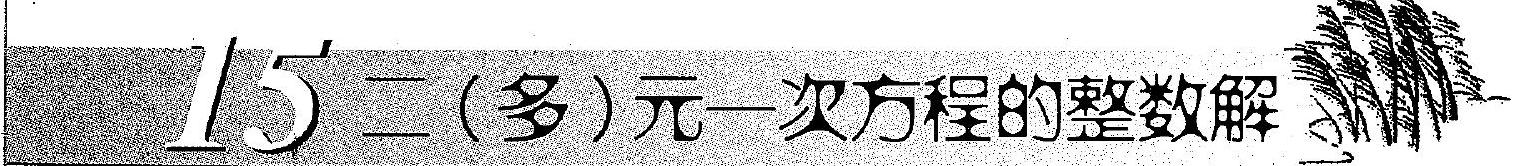
\includegraphics[max width=\textwidth, center]{2024_10_30_26b590fd1106d28139f0g-095}

两个黄鸲鸣澹柳,\\
一行白篤上青天,\\
窗含西岭才秋雪,\\
门泊东兵方里船。\\
--杜榑《经句》

如果一个方程(组)中,未知数的个数多于方程的个数,那么称这样的方程(组)为不定方程(组)。例如,方程 $8 x+6 y=46$ 为二元一次不定方程,方程组 $\left\{\begin{array}{l}x+y+z=100, \\ x+3 y+2 z=180\end{array}\right.$ 是三元一次不定方程组。

不定方程(组)的解一般是不确定的。一个不定方程总有无穷多组解,但若讨论一个整系数的不定方程的整数解或正整数解,则不定方程(组)的解有三种可能,有无数组解,或有限组解,或无解。

例1 求方程 $2 x+6 y=9$ 的整数解。\\
解 观察方程, 发现方程左边, 不论 $x, y$ 取何整数, $2 x+6 y$ 是偶数, 但方程的右边是 9 , 为奇数. 所以,不存在整数 $x, y$ 使得 $2 x+6 y=9$ 。

故此方程无整数解。\\
说明 例1告诉我们,二元一次不定方程并非都有整数解。当方程 $a x+$ $b y=c$ 中整数 $a$ 与 $b$ 的最大公约数 $d(d \geqslant 2)$ 不是 $c$ 的因数时, 此方程无整数解,如 $3 x+12 y=8$ 无整数解。一般地,我们有结论:若整系数方程 $a x+$ $b y=c$ 有整数解, 则 $a$ 与 $b$ 的最大公约数 $d$ 整除 $c$; 反之, 若其最大公约数 $d$ 整除 $c$ ,则此方程一定有整数解。这样的解可以表示出来吗?

例 2 求方程 $2 x-5 y=4$ 的全部整数解。\\
解法 1 原方程化为 $x=\frac{4+5 y}{2}$ 。 即 $x=2+\frac{5 y}{2}$ 。

业务:初高中联赛班、培优班、美国高中数学、教师培训、机构教学产品研发、讲义资料出售等\\
显然 $y$ 只能取偶数,如 $y$ 取 $\cdots,-2,0,2, \cdots$ 等,则 $x$ 分别为 $\cdots,-3,2$ , $7, \cdots$ 。

容易得到这个不定方程的解, $\cdots,\left\{\begin{array}{l}x=-3, \\ y=-2,\end{array}\left\{\begin{array}{l}x=2, \\ y=0,\end{array} \quad\left\{\begin{array}{l}x=7, \ldots \\ y=2,\end{array}\right.\right.\right.$.\\
解法 2 先由观察法,得 $\left\{\begin{array}{l}x=7, \\ y=2\end{array}\right.$ 是此方程的一组解(称其为特解)。为了求出全部整数解,设 $\left\{\begin{array}{l}x=7+m , \\ y=2+n\end{array}(m, n\right.$ 为整数 $)$.

代人原方程,得 $2(7+m)-5(2+n)=4$ ,即 $\frac{m}{5}=\frac{n}{2}$ 。\\
设比值为整数 $t$ ,得

\begin{align*}
\left\{\begin{array}{l}
x=7+5 t, \\
y=2+2 t
\end{array} \text { ( } t \text { 为整数 }\right) .
\end{align*}

这就是方程 $2 x-5 y=4$ 的全部整数解。\\
恰似"两个黄檞" $x, y$ "鸣翠柳","一行白鹭上青天" $(x=7+5 t, y=2+$ $2 t, t$ 为整数)

说明 请尝试总结出求整系数方程 $a x+b y=c$ 的全部整数解的一般步骤。

例3 求不定方程 $7 x-5 y=3$ 满足 $20 \leqslant x+y \leqslant 30$ 的整数解。\\
基本思路 先判断方程是否有整数解,此方程有整数解;其次寻求特解,如 $x=9, y=12$ ,写出方程的全部整数解的表达式;利用 $20 \leqslant x+y \leqslant 30$ ,得 $t$的取值,从而求出符合题设要求的整数解。

解 因为 $(7,-5)=1$ ,所以方程有整数解。\\
由题设知 $y=\frac{7 x}{5}-\frac{3}{5}=x+\frac{2 x-3}{5}$, 取 $x=9$, 得 $y=12$, 即为方程 $7 x-$ $5 y=3$ 的一组解,所以,此方程的全部整数解为

\begin{align*}
\left\{\begin{array}{l}
x=9+5 t, \\
y=12+7 t
\end{array} \text { ( } t\right. \text { 为任意整数). }
\end{align*}

从而 $x+y=21+12 t$ 。\\
又因为 $20 \leqslant x+y \leqslant 30$, 所以有 $20 \leqslant 21+12 t \leqslant 30$, 即 $-\frac{1}{12} \leqslant t \leqslant$ $\frac{9}{12}$.

由于 $t$ 为整数, 所以 $t=0$, 得 $x=9, y=12$.

故所求的整数解为 $\left\{\begin{array}{l}x=9, \\ y=12 .\end{array}\right.$\\
例4 求方程 $13 x+4 y=15$ 的正整数解。\\
解 观察方程,因为 $x \geqslant 1$ ,得 $13 x \geqslant 13 ; y \geqslant 1$ ,得 $4 y \geqslant 4$ ,所以 $13 x+$ $4 y \geqslant 13+4=17>15$ 。即不存在正整数 $x, y$ ,使 $13 x+4 y=15$ 成立。

故此方程无正整数解。\\
说明 一般地,若方程 $a x+b y=c$ 中, $a>0, b>0, a+b>c$ ,则这个方程无正整数解。你可以求出方程 $13 x+4 y=15$ 的全部整数解吗?

例 5 求方程 $3 x+5 y=31$ 的正整数解。\\
基本思路 先求出方程 $3 x+5 y=31$ 的全部整数解 $\left\{\begin{array}{l}x=7+5 k, \\ y=2-3 k\end{array}(k\right.$ 为任意整数), 从而得 $\left\{\begin{array}{l}7+5 k>0, \\ 2-3 k>0,\end{array}-\frac{7}{5}<k<\frac{2}{3}\right.$. 于是有 $k=0$ ,或 $k=-1$ 。

解 因为 $(3,5)=1$ ,所以方程有整数解。\\
由 $x=10-y+\frac{1-2 y}{3}$ 知取 $y=2$, 得 $x=7$, 即 $\left\{\begin{array}{l}x=7, \\ y=2\end{array}\right.$ 为方程的一组解.所以此方程的全部整数解为 $\left\{\begin{array}{l}x=7+5 k, \\ y=2-3 k,\end{array}(k\right.$ 为整数 $)$

由 $7+5 k>0$, 且 $2-3 k>0$, 得 $-\frac{7}{5}<k<\frac{2}{3}$, 所以整数 $k=-1$ 或 0 .\\
当 $k=-1$ 时, $x=2, y=5$ 。\\
当 $k=0$ 时, $x=7, y=2$ 。\\
故所求方程的正整数解为

\begin{align*}
\left\{\begin{array} { l } 
{ x = 7 , } \\
{ y = 2 ; }
\end{array} \quad \left\{\begin{array}{l}
x=2 \\
y=5
\end{array}\right.\right.
\end{align*}

例 6 一支科学考察队前往某条河流的上游去考察一个生态区。他们出发后以每天 17 km 的速度前进,沿河岸向上游行进若干天后到达目的地,然后在生态区考察了若干天,完成任务后以每天 25 km 的速度返回。在出发后的第 60 天,考察队行进了 24 km 后回到出发点。试问:科学考察队在生态区考察了多少天?

基本思路 考察队 $x$ 天到生态区,考察了 $y$ 天,满足 $42 x+25 y=1499$ 。由 $x, y$ 为正整数及方程的全部解表达式,得 $t=1$ ,从而得 $x$ 与 $y$ 。

解 设考察队到生态区用了 $x$ 天,考察了 $y$ 天,则

\begin{align*}
17 x=25(60-x-y)-1 \text {, 即 } 42 x+25 y=1499 \text {. }
\end{align*}

业务:初高中联赛班、培优班、美国高中数学、教师培训、机构教学产品研发、讲义资料出售等\\
解得 $\left\{\begin{array}{l}x=25 t-3, \\ y=65-42 t\end{array}\right.$ ( $t$ 为整数)。\\
由 $\left\{\begin{array}{l}25 t-3>0, \\ 65-42 t>0,\end{array}\right.$ 解得 $\frac{3}{25}<t<\frac{65}{42}$, 所以 $t=1$.\\
于是, $\left\{\begin{array}{l}x=22, \\ y=23 .\end{array}\right.$\\
答:科学考察队在生态区考察了 23 天.\\
例7 如果三个既约真分数 $\frac{2}{3}, \frac{a}{4}, \frac{b}{6}$ 的分子都加上 $b$ ,这时得到的三个分数的和为 6 , 求这三个既约真分数的积.

解 由题意,我们有 $\frac{2+b}{3}+\frac{a+b}{4}+\frac{b+b}{6}=6$ ,整理得

\begin{align*}
3 a+11 b=64
\end{align*}

问题转化为求 $3 a+11 b=64$ 的正整数解.\\
由 $3 a+11 b=64$ 得 $a=\frac{64-11 b}{3}$, 从而

\begin{align*}
a=21-4 b+\frac{1+b}{3}
\end{align*}

令 $b=2$ ,得 $a=14 ,$ 则这个不定方程有一组整数解 $\left\{\begin{array}{l}a=14 , \\ b=2 ,\end{array}\right.$ 从而它的所有整数解为

\begin{align*}
\left\{\begin{array}{l}
a=14+11 k, \\
b=2-3 k
\end{array} \text { ( } k\right. \text { 为任意整数). }
\end{align*}

令 $a>0, b>0$ ,得不等式组

\begin{align*}
\left\{\begin{array}{l}
14+11 k>0 \\
2-3 k>0
\end{array}\right.
\end{align*}

解得 $-\frac{14}{11}<k<\frac{2}{3}$, 从而 $k=0$ 或 -1 . 因此, 这个方程有两组正整数解

\begin{align*}
\left\{\begin{array} { l } 
{ a = 1 4 , } \\
{ b = 2 , }
\end{array} \text { 和 } \left\{\begin{array}{l}
a=3, \\
b=5 .
\end{array}\right.\right.
\end{align*}

注意 $\frac{a}{4}$ 与 $\frac{b}{6}$ 为既约真分数,所以 $a=3, b=5$ 是它的唯一解.

因此所求的积为 $\frac{2}{3} \times \frac{3}{4} \times \frac{5}{6}=\frac{5}{12}$.\\
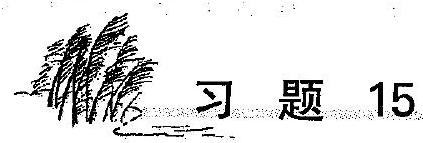
\includegraphics[max width=\textwidth, center]{2024_10_30_26b590fd1106d28139f0g-099(1)}

I 求方程 $4 x+10 y=34$ 的整数解.\\
2. 有一个两位数,加上 54 以后,十进位上的数字和个位上的数字恰好互换位置,求这个两位数。\\
(3)求方程 $5 x-3 y=-7$ 的正整数解。

4 求不定方程 $5 x-3 y=16$ 的最小正整数解。\\
[5 小凯驾车在公路上匀速行驶,他看到里程碑上的数是两位数,一小时后看到里程碑上的数恰是第一次看到的数颠倒了顺序的两位数;再过一小时后,第三次看到里程碑上的数又恰好是第一次见到的两位数字之间添加上一个 0 的三位数。问:这三块里程碑上的数各是多少?\\
6 6 将一枚六个面编号分别为 $1,2,3,4,5,6$ 的质地均匀的正方体骰子先后投掷两次,记第一次掷出的点数为 $a$ ,第二次郑出的点数为 $b$ ,则使关于 $x, y$ 的方程组 $\left\{\begin{array}{l}a x+b y=3 \\ x+2 y=2\end{array}\right.$ 只有正数解的 $a$ 与 $b$ 的概率为 ( ).\\
(A) $\frac{1}{12}$\\
(B) $\frac{2}{9}$\\
(C) $\frac{5}{18}$\\
(D) $\frac{13}{36}$\\
(2009 年全国初中数学竞赛题)\\
7青求方程 $(|x|+1)(|y|-3)=5$ 的整数解的个数。\\
8 8 — 一个箱子中装有若干只蜘蛛与蟋蟀,每只蜘蛛 8 条腿,每只蟋蟀 6 条腿。已知箱内的蜘蛛和蟋蟀共有 46 条腿,问其中蜘蛛和蟋蟀各有多少只?\\
9 一个盒子里装有不多于 200 粒棋子,如果每次 2 粒, 3 粒, 4 粒或 6 粒地取出,最终盒内都剩—粒棋子;如果每次 11 粒地取出,那么正好取完。盒子里共有多少粒棋子?\\
10. 小明玩套圈游戏,套中小鸡得 9 分,套中小猴得 5 分,套中小狗得 2 分.小明共套 10 次,每次都套中了,每个小玩具都至少被套中一次。小明套 10次共得 61 分,问:小鸡被套中几次?\\
11(1)如图,现有 $19^{\circ}$ 的"模板",请你设计一种办法,只用这个"模板"和铅笔在纸上画出 $1^{\circ}$ 的角来;\\
(2)现有一个 $17^{\circ}$ 的"模板"与铅笔,你能否\\
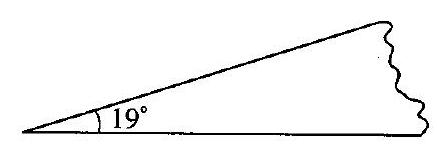
\includegraphics[max width=\textwidth, center]{2024_10_30_26b590fd1106d28139f0g-099}\\
(第 11 题)\\
15 二(多)元一次方程的整数解

全国小学奥数群:221739457,全国初中奥数学生群:253736211,全国高中奥数学生群591782992全国初中奥数教练群112464128,全国高中奥数教练群195949359\\
竞赛公众号:新浪微博@郑剑雄 微信:v136257437 QQ:136257437\\
业务:初高中联赛班、培优班、美国高中数学、教师培训、机构教学产品研发、讲义资料出售等\\
在纸上画出一个 $1^{\circ}$ 的角来?\\
(3)用一个 $21^{\circ}$ 的"模板"与铅笔,你能否在纸上画出一个 $1^{\circ}$ 的角来?\\
对于(2)、(3)两问,如果能,请你简述画法步骤;如果不能,请你说明理由。

\section*{知体操}
The real question is not whether machines think, but whether men do.真正的问题并不是机器是否思考,而是人类是否思考。\\
——斯金纳

\section*{一元二次方程的整数根}
白露收残暑,清风社晩霞。绿杨堤怑闹荷花。

件愎《南歌子

恰是一元二次方程"闹荷花"。对于有理系数的一元二次方程 $a x^{2}+b x+$ $c=0\left(a, b, c\right.$ 为有理数), 如果此方程有整数根, 那么判别式 $\Delta=b^{2}-4 a c$ 必须是一个完全平方数,即有有理数 $m$ ,使得 $b^{2}-4 a c=m^{2}$ ,反之,未必得到方程有整数根。

解决一元二次方程整数根问题,通常直接考虑有理数与实数的关系,或者因式分解,或者利用一元二次方程的判别式与求根公式,或者运用根与系数关系式,或者转化为讨论一元二次函数的取值范围,或者运用配方,或者运用整数的若干基本性质。

例1 已知关于 $x$ 的方程 $x^{2}+(a-6) x+a=0$ 的两根都是整数, 求 $a$的值。

基本思路 利用根与系数的关系消去 $a$ ,得 $\left(x_{1}+1\right)\left(x_{2}+1\right)=7$ ,因数分解;或用判别式 $\Delta=m^{2}$ ( $m$ 为整数),及平方差公式进行部分因式分解,然后再因数分解。\\
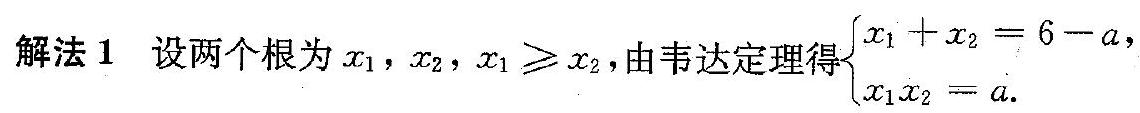
\includegraphics[max width=\textwidth]{2024_10_30_26b590fd1106d28139f0g-101}两式中消去 $a$ 得 $x_{1} x_{2}+x_{1}+x_{2}=6,\left(x_{1}+1\right)\left(x_{2}+1\right)=7$ 。

所以 $\left\{\begin{array}{l}x_{1}+1=7, \\ x_{2}+1=1\end{array}\right.$ 或 $\left\{\begin{array}{l}x_{1}+1=-1, \\ x_{2}+1=-7,\end{array}\right.$ 解得 $\left\{\begin{array}{l}x_{1}=6, \\ x_{2}=0\end{array}\right.$ 或 $\left\{\begin{array}{l}x_{1}=-2, \\ x_{2}=-8 .\end{array}\right.$\\
所以 $a=x_{1} x_{2}=0$ 或 16 。\\
解法2 由题意知 $\Delta=(a-6)^{2}-4 a=(a-8)^{2}-28=m^{2}$ ( $m$ 为整数),则有 $(a-m-8)(a+m-8)=28$, 且由 $a-m$ 与 $a+m$ 同奇偶知 $a-m-8, a+$

业务:初高中联赛班、培优班、美国高中数学、教师培训、机构教学产品研发、讲义资料出售等 $m-8$ 同奇偶, 所以 $\left\{\begin{array}{l}a-m-8=2, \\ a+m-8=14,\end{array}\right.$ 或 $\left\{\begin{array}{l}a-m-8=-14, \\ a+m-8=-2,\end{array}\right.$ 从而 $a=0$ 或 16 .

例2 已知方程 $a^{2} x^{2}-\left(3 a^{2}-8 a\right) x+2 a^{2}-13 a+15=0$ (其中 $a$ 是非负整数)至少有一个整数根,求 $a$ 的值。

解 根据题意知 $a \neq 0$ ,且有

\begin{align*}
a^{2} x^{2}-a(3 a-8) x+(2 a-3)(a-5)=0,
\end{align*}

因式分解得

解得

\begin{align*}
\begin{gathered}
(a x-2 a+3)(a x-a+5)=0, \\
x=2-\frac{3}{a}, \text { 或 } x=1-\frac{5}{a} .
\end{gathered}
\end{align*}

因为原方程至少有一个整数根,所以 $a$ 必为 $1,3,5$ ,即

\begin{align*}
a=1 \text {, 或 } a=3 \text {, 或 } a=5 \text {. }
\end{align*}

说明 运用因式分解是处理有关一元二次方程整数根的基本思路之一。\\
例3 关于 $x, y$ 的方程 $x^{2}+x y+2 y^{2}=29$ 的整数解 $(x, y)$ 的组数为\\
(A) 2 组\\
(B) 3 组\\
(C) 4 组\\
(D) 无穷多组\\
(2009 年全国初中数学竞赛题)\\
基本思路 看作关于 $x$ 的一元二次方程, 用判别式 $\geqslant 0$ 且为完全平方数,列表枚举。

解 可将原方程视为关于 $x$ 的二次方程,将其变形为

\begin{align*}
x^{2}+y x+\left(2 y^{2}-29\right)=0 .
\end{align*}

由于该方程有整数根,则判别式 $\Delta \geqslant 0$ ,且是完全平方数.\\
由

\begin{align*}
\Delta=y^{2}-4\left(2 y^{2}-29\right)=-7 y^{2}+116 \geqslant 0,
\end{align*}

解得 $y^{2} \leqslant \frac{116}{7} \approx 16.57$. 于是

\begin{center}
\begin{tabular}{|c|c|c|c|c|c|}
\hline
$y^{2}$ & 0 & 1 & 4 & 9 & 16 \\
\hline
$\Delta$ & 116 & 109 & 88 & 53 & 4 \\
\hline
\end{tabular}
\end{center}

显然,只有 $y^{2}=16$ 时, $\Delta=4$ 是完全平方数,符合要求。\\
当 $y=4$ 时,原方程为 $x^{2}+4 x+3=0$ ,此时 $x_{1}=-1 , x_{2}=-3$ ;\\
当 $y=-4$ 时,原方程为 $x^{2}-4 x+3=0$, 此时 $x_{3}=1, x_{4}=3$ 。

所以,原方程的整数解为

\begin{align*}
\left\{\begin{array} { l } 
{ x _ { 1 } = - 1 , } \\
{ y _ { 1 } = 4 ; }
\end{array} \quad \left\{\begin{array} { l } 
{ x _ { 2 } = - 3 , } \\
{ y _ { 2 } = 4 ; }
\end{array} \quad \left\{\begin{array} { l } 
{ x _ { 3 } = 1 , } \\
{ y _ { 3 } = - 4 ; }
\end{array} \quad \left\{\begin{array}{l}
x_{4}=3 \\
y_{4}=-4
\end{array}\right.\right.\right.\right.
\end{align*}

例4 已知方程 $x^{2}-6 x-4 n^{2}-32 n=0$ 的根都是整数,求整数 $n$ 的值。\\
解 由题中方程进行配方得

\begin{align*}
\left(x^{2}-6 x+9\right)-\left(4 n^{2}+32 n+64\right)+55=0
\end{align*}

即

\begin{align*}
(2 n+8)^{2}-(x-3)^{2}=55
\end{align*}

则有

\begin{align*}
\begin{aligned}
& \left\{\begin{array}{l}
|2 n+8|-|x-3|=1, \\
|2 n+8|+|x-3|=55 ;
\end{array}, \quad\left\{\begin{array}{l}
|2 n+8|-|x-3|=55, \\
|2 n+8|+|x-3|=1 ;
\end{array}\right.\right. \\
& \left\{\begin{array}{l}
|2 n+8|-|x-3|=5, \\
|2 n+8|+|x-3|=11 ;
\end{array}, \quad\left\{\begin{array}{l}
|2 n+8|-|x-3|=11, \\
|2 n+8|+|x-3|=5
\end{array}\right.\right.
\end{aligned}
\end{align*}

解得

\begin{align*}
n_{1}=10, n_{2}=-18, n_{3}=0, n_{4}=-8
\end{align*}

所以,满足题意的整数 $n$ 可以是 $-18,-8,0,10$.\\
思考 你能用其他方法来解此例吗?试比较各种方法的适用性和简捷性。

例5 已知三个整数 $a, b, c$ 之和为 13 , 且 $\frac{b}{a}=\frac{c}{b}$, 求 $a$ 的最大值和最小值, 并求出此时相应的 $b$ 与 $c$ 的值.

解 设 $\frac{b}{a}=\frac{c}{b}=x$ ,则 $b=a x, c=a x^{2}$ ,于是由 $a+b+c=13$ ,得

\begin{align*}
a\left(x^{2}+x+1\right)=13
\end{align*}

因为 $a \neq 0$ ,所以

\begin{align*}
x^{2}+x+1=\frac{13}{a}
\end{align*}

又 $a, b, c$ 是整数, 那么上述方程的解必为有理数, 所以有

\begin{align*}
\Delta=1-4\left(1-\frac{13}{a}\right)=\frac{52}{a}-3 \geqslant 0
\end{align*}

解得 $1 \leqslant a \leqslant \frac{52}{3}$, 且 $\sqrt{\Delta}$ 为有理数.\\
因此, $1 \leqslant a \leqslant 16$ 。\\
当 $a=1$ 时, $x^{2}+x+1=13$, 解得 $x_{1}=-4, x_{2}=3$,

业务:初高中联赛班、培优班、美国高中数学、教师培训、机构教学产品研发、讲义资料出售等则 $a_{\text {min }}=1, b=-4, c=16$ ,或 $a_{\text {min }}=1, b=3, c=9$ 。

当 $a=16$ 时, $x^{2}+x+\frac{3}{16}=0$ ,解得 $x_{1}=-\frac{3}{4}, x_{2}=-\frac{1}{4}$ ,则 $a_{\text {max }}=16, b=-12, c=9$ ,或 $a_{\text {max }}=16, b=-4, c=1$ 。

例 6 若 $1 \leqslant p \leqslant 20,1 \leqslant q \leqslant 10$ ,且方程 $4 x^{2}-p x+q=0$ 的两根均为奇数,求此方程的根。

解 设 $x_{1}, x_{2}$ 为方程的两个根,则

\begin{align*}
x_{1}+x_{2}=\frac{p}{4}, x_{1} x_{2}=\frac{q}{4} .
\end{align*}

因为 $x_{1}, x_{2}$ 均为奇数, 所以 $x_{1}+x_{2}$ 为偶数, $x_{1} x_{2}$ 为奇数.\\
又 $1 \leqslant p \leqslant 20,1 \leqslant q \leqslant 10$, 则

\begin{align*}
\begin{gathered}
\frac{1}{4} \leqslant \frac{p}{4} \leqslant 5, \frac{1}{4} \leqslant \frac{q}{4} \leqslant \frac{5}{2} . \\
\frac{q}{4}=1, q=4 .
\end{gathered}
\end{align*}

由方程的判别式 $\Delta=p^{2}-16 q \geqslant 0$ 得 $p \geqslant 8$,

从而

\begin{align*}
\frac{p}{4} \geqslant 2 .
\end{align*}

又 $\frac{p}{4}$ 是偶数且 $\frac{p}{4} \leqslant 5$, 则 $\frac{p}{4}=2$ 或 4 , 即 $p=8$, 或 $p=16$.\\
当 $p=8$ 时, $x_{1}=x_{2}=1$ ,符合题意;\\
当 $p=16$ 时, $x_{1}$ 与 $x_{2}$ 均为无理数,不合题意,舍去。\\
故原方程的根为 $x_{1}=x_{2}=1$ 。\\
例7 已知关于 $x$ 的一元二次方程 $x^{2}+c x+a=0$ 的两个整数根恰好比方程 $x^{2}+a x+b=0$ 的两个根都大 1 , 求 $a+b+c$ 的值。(2011 年全国初中数学竞赛题)

基本思路 由题意列出 $\alpha+\beta=-a,(\alpha+1)(\beta+1)=a$ ,得 $(\alpha+2)(\beta+2)=$ 3 ,对于 $\alpha \leqslant \beta$ ,得 $\alpha$ 与 $\beta$ 的值,从而求出 $a, b, c$ 。

解 设方程 $x^{2}+a x+b=0$ 的两个根为 $\alpha, \beta$ ,其中 $\alpha, \beta$ 为整数,且 $\alpha \leqslant \beta$ ,则方程 $x^{2}+c x+a=0$ 的两根为 $\alpha+1, \beta+1$ 。

由题意得

\begin{align*}
\alpha+\beta=-a,(\alpha+1)(\beta+1)=a
\end{align*}

两式相加得

\begin{align*}
\alpha \beta+2 \alpha+2 \beta+1=0
\end{align*}

业务:初高中联赛班、培优班、美国高中数学、教师培训、机构教学产品研发、讲义资料出售等\\
即

\begin{align*}
(\alpha+2)(\beta+2)=3,
\end{align*}

所以

\begin{align*}
\left\{\begin{array} { l } 
{ \alpha + 2 = 1 , } \\
{ \beta + 2 = 3 ; }
\end{array} \text { 或 } \left\{\begin{array}{l}
\alpha+2=-3 ; \\
\beta+2=-1 .
\end{array}\right.\right.
\end{align*}

解得 $\left\{\begin{array}{l}\alpha=-1, \text { 或 }_{\alpha}=-5, \\ \beta=1\end{array}\right.$,\\
又因为 $a=-(\alpha+\beta), b=\alpha \beta, c=-[(\alpha+1)+(\beta+1)]$, 所以 $a=0, b=$ $-1, c=-2$ ;或者 $a=8, b=15, c=6$ 。

故 $a+b+c=-3$ ,或 29 。\\
例 8 试求方程 $4 x^{2}-40[x]+51=0$ 的全部实数解,此处 $[x]$ 表示小于或等于实数 $x$ 的最大整数。

解 尝试转化原问题为一元二次方程整数根的问题。\\
令 $x=[x]+B$, 这里 $0 \leqslant B<1$, 则 $[x] \leqslant x<[x]+1$.\\
于是

\begin{align*}
4 x^{2}-40 x+51 \leqslant 4 x^{2}-40[x]+51=0
\end{align*}

且

\begin{align*}
4 x^{2}-40(x-1)+51>4 x^{2}-40[x]+51=0
\end{align*}

从而可知满足原方程的实数 $x$ 必须满足

\begin{align*}
\left\{\begin{array}{l}
4 x^{2}-40 x+51 \leqslant 0 \\
4 x^{2}-40(x-1)+51>0
\end{array}\right.
\end{align*}

解得

\begin{align*}
\frac{3}{2} \leqslant x<\frac{7}{2}, \text { 或 } \frac{13}{2}<x \leqslant \frac{17}{2}, \tag{1}
\end{align*}

且有

\begin{align*}
[x]=2,3,7,8
\end{align*}

当 $[x]=2$ 时, 则由 $4 x^{2}=29$, 得 $x=\frac{\sqrt{29}}{2}$. 因 $2<\frac{\sqrt{29}}{2}<3$, 所以, $x=$ $\frac{\sqrt{29}}{2}$ 是原方程的实数解。

当 $[x]=3$ 时, 同理得 $x=\frac{\sqrt{69}}{2}$. 但 $x=\frac{\sqrt{69}}{2}>4$, 这与 $[x]=3$ 不符,所以 $x=\frac{\sqrt{69}}{2}$ 不是原方程的解.

当 $[x]=7$ 时, 由 $4 x^{2}=229$, 得 $x=\frac{\sqrt{229}}{2}$. 因 $7<\frac{\sqrt{229}}{2}<8$, 所以 $x=$ $\frac{\sqrt{229}}{2}$ 是原方程的实数解。

业务:初高中联赛班、培优班、美国高中数学、教师培训、机构教学产品研发、讲义资料出售等\\
当 $[x]=8$ 时, 由 $4 x^{2}=269$, 得 $x=\frac{\sqrt{269}}{2}$. 因 $8<\frac{\sqrt{269}}{2}<9$, 所以 $x=$ $\frac{\sqrt{269}}{2}$ 也为原方程的实数解。

故原方程的实数解为 $x=\frac{\sqrt{29}}{2}, \frac{\sqrt{229}}{2}, \frac{\sqrt{269}}{2}$.\\
例 9 求满足 $2 p^{2}+p+8=m^{2}-2 m$ 的所有素数 $p$ 和正整数 $m$ 。(2010 年全国初中数学竞赛题)

基本思路 利用 $p$ 为素数及数的整除性,得 $p \mid(m-4)$ 或 $p \mid(m+2)$ 。采用估算法求出 $p=5$ 。

解 由题设得 $p(2 p+1)=(m-4)(m+2)$ ,所以 $p \mid(m-4)(m+2)$ 。由于 $p$ 是素数,故 $p \mid(m-4)$ ,或 $p \mid(m+2)$ 。\\
(1) 若 $p \mid(m-4)$ ,令 $m-4=k p$ ,于是 $m+2>k p$ ,

\begin{align*}
3 p^{2}>p(2 p+1)=(m-4)(m+2)>k^{2} p^{2}
\end{align*}

得 $k^{2}<3$ ,从而 $k=1$ 或 $k=-1$ 。\\
所以 $\left\{\begin{array}{l}m-4=p, \\ m+2=2 p+1,\end{array}\right.$ 解 得 $\left\{\begin{array}{l}p=5, \\ m=9 ;\end{array}\right.$ 或 $\left\{\begin{array}{l}m-4=-p, \\ m+2=-(2 p+1),\end{array}\right.$ 解 得 $\left\{\begin{array}{l}p=-7, \\ m=11,\end{array}\right.$ 不符题意, 舍去.\\
(2)若 $p \mid(m+2)$ ,令 $m+2=k p, k$ 是正整数。\\
当 $p>5$ 时, 有 $m-4=k p-6>k p-p=p(k-1)$,

\begin{align*}
3 p^{2}>p(2 p+1)=(m-4)(m+2)>k(k-1) p^{2}
\end{align*}

得 $k(k-1)<3$ ,从而 $k=1$ ,或 2.\\
由于 $p(2 p+1)=(m-4)(m+2)$ 是奇数, 所以 $k \neq 2$, 从而 $k=1$.\\
于是 $\left\{\begin{array}{l}m-4=2 p+1, \\ m+2=p,\end{array}\right.$ 这不可能.\\
当 $p=5$ 时, $m=9$ ;当 $p=3, m^{2}-2 m=29$ ,无正整数解;当 $p=2$ 时, $m^{2}-2 m=18$ ,无正整数解。

综上所述, 所求素数 $p=5$, 正整数 $m=9$ 。

\section*{习 题 16}
1 设 $a, b$ 为整数,已知关于 $x$ 的方程

\begin{align*}
\frac{1}{4} x^{2}-a x+a^{2}+a b-a-b-1=0
\end{align*}

有两个相同的实根,求 $a-b$ 的值。\\
2 若关于 $x$ 的方程 $r x^{2}-(2 r+7) x+(r+7)=0$ 的根是正整数, 求整数 $r$ 的值.\\
3 已知方程 $\sqrt{x}+3 \sqrt{y}=\sqrt{300}$, 求此方程的正整数解的组数.\\
4. 已知 $a, b$ 都是正整数,试问关于 $x$ 的方程 $x^{2}-a b x+\frac{1}{2}(a+b)=0$ 是否有两个整数解?如果有,请把它们求出来:如果没有,请给出证明。(2007年全国初中数学竞赛题)\\
5 已 已知 $a_{1}, a_{2}, a_{3}, a_{4}, a_{5}$ 是满足条件 $a_{1}+a_{2}+a_{3}+a_{4}+a_{5}=9$ 的五个不同的整数,若 $b$ 是关于 $x$ 的方程 $\left(x-a_{1}\right)\left(x-a_{2}\right)\left(x-a_{3}\right)\left(x-a_{4}\right)\left(x-a_{5}\right)=$ 2009 的整数根,求 $b$ 的值。(2009 年全国初中数学竞赛题)\\
6 . 如图,正方形 $E F G H$ 内接于 $\triangle A B C$ ,设 $B C=\overline{a b}$ ( $\overline{a b}$ 是一个两位数), $E F=c$ ,三角形高 $A D=d$ 。 已知 $a, b, c, d$ 是从小到大的四个连续正整数,试求 $\triangle A B C$ 的面积。\\
7 若 $m, n$ 都是整数,求证:方程 $x^{2}+10 m x$ $5 n+3=0$ 没有整数根。\\
8设方程 $a x^{2}+b x+c=0$ ,系数 $a, b, c$ 都是奇数,证明:这个方程无整数根。\\
9 是否存在素数 $p, q$ ,使得关于 $x$ 的一元二次\\
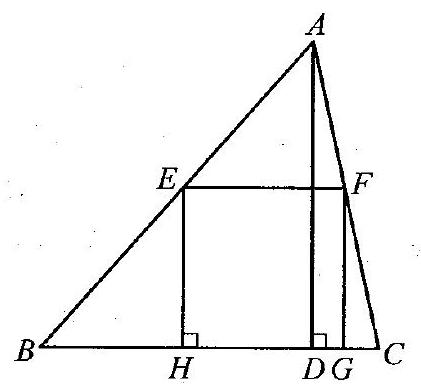
\includegraphics[max width=\textwidth, center]{2024_10_30_26b590fd1106d28139f0g-107}

第 6 题

方程 $p x^{2}-q x+p=0$ 有有理数根?(2008年全国初中数学竞赛题) 10 求方程 $x^{2}+y^{2}=208(x-y)$ 的所有正整数解。(2008 年全国初中数学竞赛题)

\section*{心智体操}
\section*{机 智}
歌德有一天晚上到效外散步,在一条仅能通行一人的小道上,迎面碰上个仇家。这人一见歌德便大声说:"我决不会给猪让路。"歌德微笑着说:"我会。"接着侧过身子站到一边。

英国首相丘吉尔到美国访问,在众议院发表演说后走下讲台。一位反对他的女议员气冲冲地走到他的面前说:"阁下,如果我是你妻子的话,我会在你的咖啡里下毒药。"丘吉尔平静地看着这位女议员说:"夫人,如果我是你丈夫的话,我会喝掉它。"

利用一元二次方程知识,可以解决许多或涉及数学本身的、或涉及生活实际的、或涉及科学技术方面的问题。

运用一元二次方程解决问题的过程,就是我们常说的数学建模过程。其解题过程可以用下面的流程图表示:\\
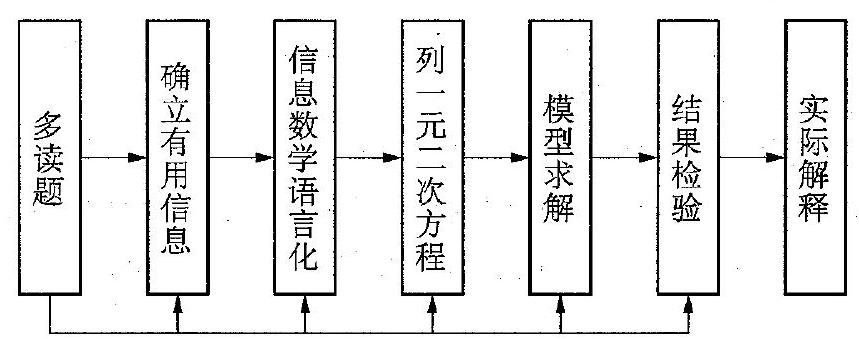
\includegraphics[max width=\textwidth, center]{2024_10_30_26b590fd1106d28139f0g-108}

在这里要特别强调的是"多读题"。根据大量的学生在解答应用题的实际过程表明,运用一元二次方程解决应用问题的难点,不在于解一元二次方程,而在于多读题,深刻理解题意,转换等量关系。

通过多读题,可以知道实际应用问题中包含的背景,注意题中背景,不是现实生活中的背景;

通过多读题,确立题中每句话的数学含意;\\
通过多读题,大胆用字母表示各对象,仔细列出关系式,把相关文字语言数学化;

通过多读题,整体把握数学化语言(数学式)之间的关系;\\
通过多读题,校正建立的一元二次方程式;

通过多读题,确立方程的解的实际有效性。\\
实践下列几例,以理解上述观念。从而感悟:数学,说不尽,无穷好。\\
例1 今有方池一丈,葭(jī̄)生其中央,出水一尺,引葭赴岸,适与水齐,问水深蓡长各几何?(摘自《九章算术》)\\
(翻译成现代语言,就是:有一个正方形的池塘,边长为一丈(我国古代长度单位:一丈等于 10 尺,现在的 1 米等于 3 尺),池中央生长着一根芦苇,比水面高出一尺,把芦苇拉到岸边,恰与水面平齐。问水有多深?芦苇有多长?)

基本思路 如图,令 $A C=x$ ,则对直角\\
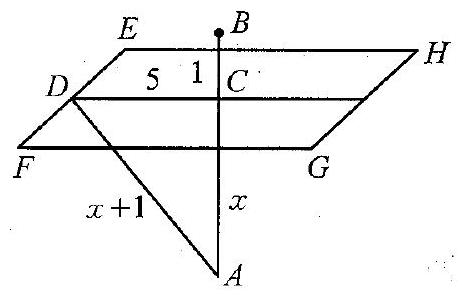
\includegraphics[max width=\textwidth, center]{2024_10_30_26b590fd1106d28139f0g-109}

图 17-1\\
$\triangle A C D$ 用勾股定理得 $(x+1)^{2}=x^{2}+5^{2}$ ,解这个方程即可。

解 如图 17-1, $E F G H$ 为正方形池塘,边长为 10 尺, $A B$ 为长在池塘中央的芦苇,高出水面 $B C=1$ 尺。设水深 $A C=x$ 尺,则芦苇长 $A B=(x+1)$ 尺,把芦苇拉到岸边点 $D$ ,即与原来的芦苇构成一个直角三角形 $A C D$ 。于是,由勾股定理得

\begin{align*}
(x+1)^{2}=x^{2}+5^{2}
\end{align*}

解得 $x=12$.\\
答:水深 1 丈 2 尺,葭长 1 丈 3 尺。\\
说明 此题载于《九章算术》一书中,《九章算术》中的二次方程的解法,早于欧洲一千多年,这是我国古代数学的重要成就。在印度也有类似的古题,印度数学家婆斯加罗(1141~1225)的著作中有一道"荷花问题":

湖平浪静出新莲,五寸婷婷出笑颜,\\
孰意风狂玉枝倒,忍看花色没波涟,\\
渔翁秋后寻根源,相距残花二尺边,\\
借问群英贤学子,水深多少在当年?\\
这个问题与《九章算术》中的"引葭赴岸"题如出一辙,但时间比"引葭赴岸"晚了一千多年(公元 $3 \sim 9$ 世纪,中国佛教盛行,中印两国之间往来频繁,这道题大约就在这时传入了印度)。

例 2 (古印度蜂群问题)有一群蜜蜂,一部分飞进了枸杞叶里,其个数等于全体总数的一半的平方根,还有全体的 $\frac{8}{9}$ 遗留在后面。此外,这群里还有一个小蜜蜂在莲花旁徘徊着,它被一个堕入香花陷吽的同伴的呻吟声所吸引。

业务:初高中联赛班、培优班、美国高中数学、教师培训、机构教学产品研发、讲义资料出售等试问这群蜜蜂共有多少个?

解 设 $x$ 表示所求的蜜蜂个数,按题意得方程

\begin{align*}
\sqrt{\frac{x}{2}}+\frac{8}{9} x+2=x
\end{align*}

令 $y=\sqrt{\frac{x}{2}}$, 得 $x=2 y^{2}$ ,则有

\begin{align*}
y+\frac{16 y^{2}}{9}+2=2 y^{2}
\end{align*}

即

\begin{align*}
2 y^{2}-9 y-18=0
\end{align*}

解得

\begin{align*}
y_{1}=6, y_{2}=-\frac{3}{2}
\end{align*}

但因 $y=\sqrt{\frac{x}{2}} \geqslant 0$ ,所以 $y_{2}=-\frac{3}{2}$ 不符合,舍去。从而由 $y_{1}=6$ 得 $x=72$ 。\\
经检验,72个蜜蜂符合要求。\\
答:这群蜜蜂一共有 72 个。\\
例 3 (欧拉与农妇卖鸡蛋问题)两个农妇一共带着 100 个鸡蛋去市场上卖,两人蛋数不同,但卖得的钱数是一样的。于是第一个农妇对第二个农妇说:"如果你的鸡蛋换给我,我可以卖得 15 个钱。"第二个农妇答道:"但是你的鸡蛋如果换给我,我就只能卖得 $6 \frac{2}{3}$ 个钱。"(这里的"钱"是指一种德国古代的货币 Kpeuzer)试问每人各有多少个鸡蛋?

解 设第一个农妇有 $x$ 个鸡蛋,那么第二个农妇有 $100-x$ 个。\\
如果第一个农妇有 $100-x$ 个鸡蛋,则她可以卖得 15 个钱。这就是说,第一个农妇所卖出鸡蛋的价格是 $\frac{15}{100-x}$.

同样地,可以求出第二个农妇卖出鸡蛋的价格是

\begin{align*}
6 \frac{2}{3} \div x=\frac{20}{3 x}
\end{align*}

现在可以确定每个农妇实际所得\\
第一个农妇: $x \cdot \frac{15}{100-x}=\frac{15 x}{100-x}$ ;\\
第二个农妇: $(100-x) \cdot \frac{20}{3 x}=\frac{20(100-x)}{3 x}$ 。\\
既然两个农妇所得相等,那么就有

即

\begin{align*}
\frac{15 x}{100-x}=\frac{20(100-x)}{3 x}
\end{align*}

\begin{align*}
x^{2}+160 x-8000=0
\end{align*}

解得

\begin{align*}
x_{1}=40, x_{2}=-200
\end{align*}

因负根在本题中没有实际意义,所以,可知第一个农妇带了 40 个鸡蛋,第二个农妇带了 60 个鸡蛋。

答:第一个农妇有 40 个鸡蛋,第二个农妇有 60 个鸡蛋。\\
说明 这个问题还可以有如下简单的解法. 这方法虽然巧妙,但不太容易想得到。

我们假设第二个农妇所有鸡蛋的数目是第一个的 $k$ 倍,她们所得钱数既然相等,则第一个农妇鸡蛋的卖价是第二个的 $k$ 倍。如果在卖出前她们两人把鸡蛋交换了,则第一个农妇的蛋数与卖价都是第二个农妇的 $k$ 倍。于是,可知第一个农妇所得钱数应该是第二个农妇的 $k^{2}$ 倍,即

解得

\begin{align*}
\begin{gathered}
k^{2}=15 \div 6 \frac{2}{3}=\frac{45}{20}=\frac{9}{4} \\
k=\frac{3}{2}
\end{gathered}
\end{align*}

现在,只要把 100 个鸡蛋分为 $3: 2$ 的比就行了。如此我们求出第一个农妇有 40 个鸡蛋,而第二个农妇有 60 个鸡蛋。

例4(名画"难题")波格达诺夫 $\cdot$ 别列斯基的名画"难题"(图 17-2),画中"难题"的内容是:

\begin{align*}
\frac{10^{2}+11^{2}+12^{2}+13^{2}+14^{2}}{365}=?
\end{align*}

画中问题利用了 $10,11,12,13,14$ 这五个数具有一种有趣的特征:

\begin{align*}
10^{2}+11^{2}+12^{2}=13^{2}+14^{2}
\end{align*}

结合 $100+121+144=365$ ,所以很容易心算出画里那个式子的结果是 2.代数使我们有办法推广这个有趣的数列特征问题。\\
这样的五个连续整数的数列是唯一的吗?还有没有其他的五个连续整数,其中前三个的平方和也等于后两个的平方和呢?

解 设 $x$ 是由大到小排列的五个数中的第二个,则有

\begin{align*}
(x-1)^{2}+x^{2}+(x+1)^{2}=(x+2)^{2}+(x+3)^{2}
\end{align*}

17 一元二次方程的应用

全国小学奥数群:221739457,全国初中奥数学生群:253736211,全国高中奥数学生群591782992全国初中奥数教练群112464128,全国高中奥数教练群195949359竞赛公众号:新浪微博@郑剑雄 微信:v136257437 QQ:136257437\\
业务:初高中联赛班、培优班、美国高中数学、教师培训、机构教学产品研发、讲义资料出售等\\
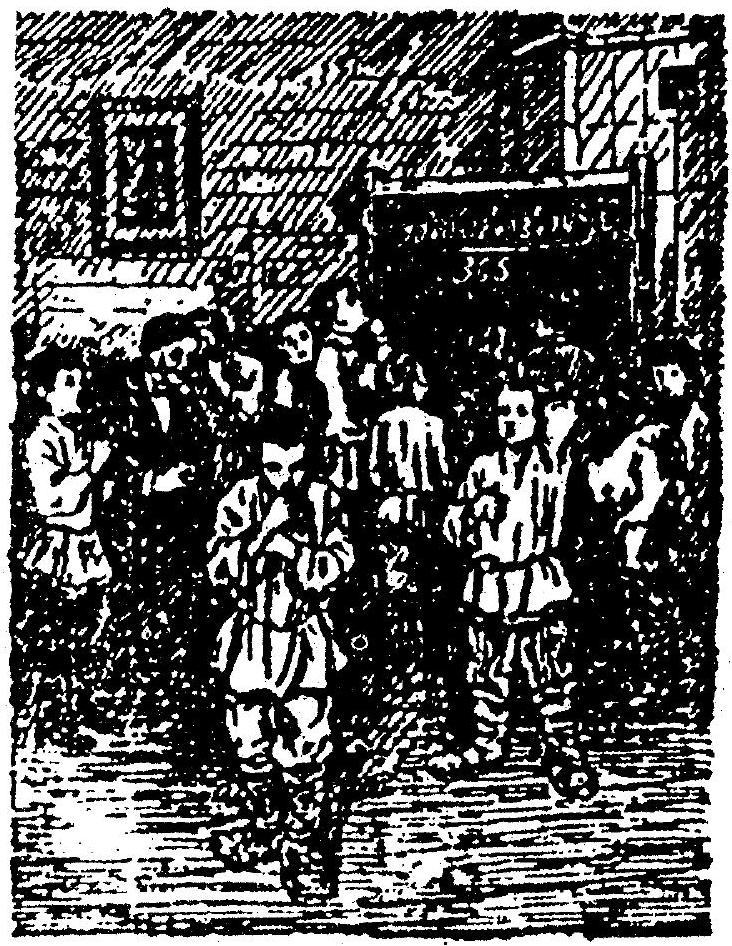
\includegraphics[max width=\textwidth, center]{2024_10_30_26b590fd1106d28139f0g-112}

图 17-2\\
整理得\\
$x^{2}-10 x-11=0$,\\
解得

\begin{align*}
x_{1}=11, x_{2}=-1
\end{align*}

所以具有所要求的数列有两组:

\begin{align*}
\begin{gathered}
10,11,12,13,14 ; \\
-2,-1,0,1,2 .
\end{gathered}
\end{align*}

思考 如果设 $x$ 表示所求由小到大五个数中的第一个,能得到同样的结果吗?请你试一试。

例 5 象棋比赛共有奇数个选手参加,每位选手都与其他选手比赛一盘,记分办法:胜一盘得 1 分,和一盘各得 0.5 分,负一盘得 0 分. 已知其中两名选手共得 8 分,其他人的平均分为整数。求参加此次比赛的选手人数。

基本思路 注意到每比赛一盘,比赛双方共得 1 分,于是可知,不论比赛的胜负状况如何,总得分应当等于比赛场数。这样就排除了"胜一盘得1分,和一盘各得 0.5 分,负一盘得 0 分"造成的不知各场比赛的胜负情况的干扰。

每位选手都与其他选手比赛一盘,共计比赛盘数也就是总得分数应如何计算呢?如果一共有 $k$ 人参加比赛,则每人都要比赛 $k-1$ 场,于是 $k$ 人比赛场

次应为 $k(k-1)$ 。但每场比赛都有 2 人参加,因此分别被两人计算过,故实际比赛场次应为 $\frac{1}{2} k(k-1)$ 。令 $x+2$ 人参加比赛, $x$ 人平均分为 $n$ ,得到方程 $x^{2}-$ $(2 n-3) x-14=0$.

解 设共有 $x+2$ 人参加比赛,则共比赛 $\frac{1}{2}(x+2)(x+1)$ 场,除 2 人外其余 $x$ 人共得分为 $\frac{1}{2}(x+2)(x+1)-8$ 分,其平均分设为 $n$ 分,则得方程

\begin{align*}
\frac{1}{2}(x+2)(x+1)-8=x n
\end{align*}

整理得

\begin{align*}
x^{2}-(2 n-3) x-14=0
\end{align*}

由于人数 $x$ 必须为正整数,且 $2 n-3$ 为整数,故 $x$ 必为 14 的正约数,即 $x$只可能等于 $1,2,7,14$ 。

又 $x$ 为奇数,故 $x=1$ 或 7 。显然 $x=1$ 不合题意, 故 $x=7$ 。\\
以 $x=7$ 检验,共计比赛 $\frac{1}{2} \times 9 \times 8=36$ (场),有 2 人共得 8 分,其余 7 人共得 28 分,平均每人得 4 分。

答:参加比赛的选手共有 9 人。\\
说明 若设人数为 $x$ 人,其余的选手每人平均得 $n$ 分,则得方程

\begin{align*}
x^{2}-(2 n+1) x+4(n-4)=0
\end{align*}

这个方程比解答中的方程较繁。为解此方程,可考虑

\begin{align*}
\Delta=(2 n+1)^{2}-16(n-4)=(2 n-3)^{2}+56
\end{align*}

为完全平方数。由于 $2 n-3$ 为奇数,则 $\Delta$ 为奇数平方,令 $\Delta=(2 m-1)^{2}(m$ 为正奇数)。于是有

\begin{align*}
\begin{aligned}
& (2 n-3)^{2}-(2 m-1)^{2}=-56 \\
& (n+m-2)(n-m-1)=-14
\end{aligned}
\end{align*}

由于 $n+m-2$ 与 $n-m-1$ 均为 14 的约数且二者奇偶性不同, 又 $n+$ $m-2>n-m-1$ ,故得

\begin{align*}
\left\{\begin{array} { l } 
{ n + m - 2 = 1 4 , } \\
{ n - m - 1 = - 1 }
\end{array} \text { 或 } \left\{\begin{array}{l}
n+m-2=7, \\
n-m-1=-2 .
\end{array}\right.\right.
\end{align*}

17 一元二次方程的应用

物理竞赛群:271751860,化学竞赛群:271751511,生物竞赛群:254139830,信息竞赛群:281798334,英语竞赛群:271750414,英语口语群:168570356,心算交流群:131033273,夏门培训机构教师招聘

业务:初高中联赛班、培优班、美国高中数学、教师培训、机构教学产品研发、讲义资料出售等解得

\begin{align*}
\left\{\begin{array} { l } 
{ n = 8 , } \\
{ m = 8 }
\end{array} \text { 或 } \left\{\begin{array}{l}
n=4, \\
m=5,
\end{array}\right.\right.
\end{align*}

其中 $n=4$ 为满足题意的解。仍得上解。\\
例6(小站设在哪里?)在一段笔直的铁路线的一边,离它 20 千米的地方有一个村子 $B$ ,如图 17-3所示。现在要设一个小站 $C$ ,使得由 $A$ 到 $B$ 的路程,沿铁路 $A C$ 走再沿公路 $C B$ 走,两段合起来所需时间最短。已知沿铁路每分钟走 0.8 千米,沿公路每分钟走 0.2 千米。问这小站应该设在哪里?\\
\includegraphics[max width=\textwidth, center]{2024_10_30_26b590fd1106d28139f0g-114}

图 17-3\\
解 我们用 $a$ 表示由 $A$ 至 $B D$ 的垂足 $D$ 间的距离 $A D$ ,用 $x$ 表示 $C D$ ,则 $A C=A D-C D=a-x$ ,而 $C B=\sqrt{C D^{2}+B D^{2}}=\sqrt{x^{2}+20^{2}}$ 。

沿铁路走 $A C$ 一段路程所需时间等于

\begin{align*}
\frac{A C}{0.8}=\frac{a-x}{0.8}
\end{align*}

沿公路走 $C B$ 一段路程所需时间等于

\begin{align*}
\frac{C B}{0.2}=\frac{\sqrt{x^{2}+20^{2}}}{0.2}
\end{align*}

而由 $A$ 到 $B$ 全路程所需时间等于

\begin{align*}
\frac{a-x}{0.8}+\frac{\sqrt{x^{2}+20^{2}}}{0.2}
\end{align*}

这个总和(用 $m$ 表示)应该是最小的。\\
于是,得方程

\begin{align*}
\frac{a-x}{0.8}+\frac{\sqrt{x^{2}+20^{2}}}{0.2}=m
\end{align*}

即

\begin{align*}
-\frac{x}{0.8}+\frac{\sqrt{x^{2}+20^{2}}}{0.2}=m-\frac{a}{0.8}
\end{align*}

两边乘以 0.8 得

\begin{align*}
-x+4 \sqrt{x^{2}+20^{2}}=0.8 m-a
\end{align*}

令 $k=0.8 m-a$ ,则有一个二次方程

解得

\begin{align*}
\begin{gathered}
15 x^{2}-2 k x+6400-k^{2}=0 \\
x=\frac{k \pm \sqrt{16 k^{2}-96000}}{15}
\end{gathered}
\end{align*}

由 $k=0.8 m-a$ ,得 $m$ 数值最小时 $k$ 也达到最小的数值,反之亦然。(应该知道: $k>0$ ,因为 $0.8 m=a-x+4 \sqrt{x^{2}+20^{2}}>a-x+x=a$ )

为使 $x$ 是实数, $16 k^{2}$ 的最小数值是 96000 , 则当 $16 k^{2}=96000$ 时, $m$ 的数值最小,由此 $k=\sqrt{6000}$ 。

所以 $x=5.16$.\\
故这个小站应该设在离 $D$ 点大约 5 千米的地方,不论 $a=A D$ 有多长。\\
但是这个解只有在 $x<a$ 时才有意义,因为在列方程式时是把 $a-x$ 这个式子看作是正数的。

若 $x=a=5.16$, 则小站根本不需要设立, 只要沿公路走向大站就行了.在距离 $a$ 短于 5.16 千米时亦是如此。

说明 本例告诉我们,在利用数学工具解决实际问题时,要对所得结果加以讨论或论证。如果忽略了应用数学工具所依据的前提,则所得结果会失去实际的意义。

例7(修建房屋)在只剩一堵墙的破屋基础上要求修建新屋(修四面墙),旧墙长 12 米,新屋面积预定为 112 平方米。这项工程的经济条件是:\\
(1)修理旧墙的费用相当于砌新墙的 $25 \%$ ;\\
(2)拆旧墙的一部分,利用旧料来砌新墙,这费用相当于用新料砌新墙的 $50 \%$ 。

问:在这情况下应以何种方式来利用旧墙最为合算?

解 设旧墙保留 $x$ 米作为第一面墙,而拆去其余 $(12-x)$ 米,所得材料用到新屋的第二面墙上来,(第二面墙长度为 $y$ 米),如图 $17-4$所示。

若新料砌新墙的费用每米为 $a$ ,则修理 $x$\\
\includegraphics[max width=\textwidth, center]{2024_10_30_26b590fd1106d28139f0g-115}

图17-4

业务:初高中联赛班、培优班、美国高中数学、教师培训、机构教学产品研发、讲义资料出售等米旧墙的费用为 $\frac{a x}{4}$ ,用旧料砌( $12-x$ )米长的新墙费用为 $\frac{a(12-x)}{2}$ ,砌第二面墙的其余部分费用为 $a[y-(12-x)]$ ,即 $a(y+x-12)$ ,砌第三面墙的费用为 $a x$ ,砌第四面墙的费用为 $a y$ 。

于是全部费用为

\begin{align*}
\begin{aligned}
S & =\frac{a x}{4}+\frac{a(12-x)}{2}+a(y+x-12)+a x+a y \\
& =\frac{a(7 x+8 y)}{4}-6 a
\end{aligned}
\end{align*}

上式在 $7 a x+8 a y$ 最小时取得最小值。\\
已知房子的面积 $x y=112$ 平方米,所以

\begin{align*}
7 a x \cdot 8 a y=112 \cdot 56 a^{2}
\end{align*}

那么 $S \geqslant \frac{1}{4} \times 2 \sqrt{7 a x \cdot 8 a y}-6 a=\frac{1}{4} \times 2 \times \sqrt{112 \cdot 56 a^{2}}-6 a$,当 $7 a x=8 a y$, 即 $y=\frac{7}{8} x$ 时 $S$ 取得最小值, 于是由 $x y=112$, 得

\begin{align*}
\frac{7}{8} x^{2}=112, x=\sqrt{128} \approx 11.3
\end{align*}

又旧墙长 12 米,那么所拆部分为 $12-x \approx 12-11.3=0.7$ (米).\\
说明 这里利用了 $a+b \geqslant 2 \sqrt{a b}$ ,等号当且仅当 $a=b$ 时成立。\\
一元二次方程知识还可以用来处理数字问题、几何问题等。\\
例8 设四位数 $\overline{a b c d}$ 是一个完全平方数,且 $\overline{a b}=2 \overline{c d}+1$ ,求这个四位数。\\
解 设 $\overline{a b c d}=m^{2}$ ,则 $32 \leqslant m \leqslant 99$ 。\\
又设 $\overline{c d}=x$, 则 $\overline{a b}=2 x+1$, 于是

即

\begin{align*}
\begin{gathered}
100(2 x+1)+x=m^{2} \\
67 \times 3 x=(m+10)(m-10)
\end{gathered}
\end{align*}

由于 67 是素数,那么 $m+10$ 与 $m-10$ 中至少有一个是 67 的倍数。\\
若 $m+10=67 k$ ( $k$ 是正整数),因为 $32 \leqslant m \leqslant 99$ ,所以 $k=1$ ,则 $m+$ $10=67$ ,即 $m=57$ 。

检验知 $57^{2}=3249$ ,不合题意,舍去。\\
若 $m-10=67 k$ ( $k$ 是正整数),同理, $k=1$ ,则 $m-10=67$ ,即 $m=77$ 。\\
所以 $\overline{a b c d}=77^{2}=5929$ 。\\
例 9 已知正 $n$ 边形共有 $n+3$ 条对角线,其周长为 $x$ ,对角线长的和为

解 正 $n$ 边形的对角线的条数为 $\frac{n(n-3)}{2}$, 那么有

得

\begin{align*}
\begin{aligned}
& \frac{n(n-3)}{2}=n+3 \\
& n^{2}-5 n-6=0
\end{aligned}
\end{align*}

解得

\begin{align*}
n=6 \text { 或 } n=-1 \text { (不合题意, 舍去). }
\end{align*}

令正六边形的边长是 $a$, 那么从一顶点出发的三条对角线长为

\begin{align*}
a \times \frac{\sqrt{3}}{2} \times 2, \sqrt{(\sqrt{3} a)^{2}+a^{2}}, a \times \frac{\sqrt{3}}{2} \times 2
\end{align*}

即

\begin{align*}
\sqrt{3} a, 2 a, \sqrt{3} a
\end{align*}

因此,正六边形的对角线长之和是 $(2 \sqrt{3} a+2 a) \times 3=6 \sqrt{3} a+6 a$.\\
于是, $\frac{y}{x}=\frac{6 \sqrt{3} a+6 a}{6 a}=1+\sqrt{3}$ 。\\
例10 一个直角三角形的边长都是整数,它的面积和周长的数值相等,试确定这个直角三角形三边的长。

解 设 $a, b$ 分别为两条直角边长,则斜边长 $c=\sqrt{a^{2}+b^{2}}$.\\
由于 $a, b, c$ 均为正整数,所以 $a \neq b$ ,不妨设 $a>b$ ,依题意有

\begin{align*}
\begin{aligned}
& a+b+\sqrt{a^{2}+b^{2}}=\frac{a b}{2} \\
& \sqrt{a^{2}+b^{2}}=\frac{a b}{2}-(a+b)
\end{aligned}
\end{align*}

两边平方整理得

即

\begin{align*}
\frac{a^{2} b^{2}}{4}-a^{2} b-a b^{2}+2 a b=0
\end{align*}

也即

\begin{align*}
a b-4 a-4 b+8=0
\end{align*}

\begin{align*}
(a-4)(b-4)=8=1 \times 8=2 \times 4,
\end{align*}

因为 $a, b$ 是正整数, $a>b$, 所以有

\begin{align*}
\left\{\begin{array} { l } 
{ a - 4 = 8 , } \\
{ b - 4 = 1 ; }
\end{array} \text { 或 } \left\{\begin{array}{l}
a-4=4, \\
b-4=2 .
\end{array}\right.\right.
\end{align*}

解得

\begin{align*}
a=12, b=5, c=13 \text {, 或 } a=8, b=6, c=10 \text {. }
\end{align*}

\begin{center}
\includegraphics[max width=\textwidth]{2024_10_30_26b590fd1106d28139f0g-117}
\end{center}

物理竞赛群:271751860,化学竞赛群:271751511,生物竞赛群:254139830,信息竞赛群:281798334,英语竞赛群:271750414,英语 $\square$ 语群:168570356,心算交流群:131033273,厦门培训机构教师招聘

业务:初高中联赛班、培优班、美国高中数学、教师培训、机构教学产品研发、讲义资料出售等\\
所以,这个直角三角形三边的长为 $(12,5,13)$ ,或 $(8,6,10)$ 。\\
例11 设 $a, b, c$ 是实数,且 $a \neq 0,(b-1)^{2}-4 a c=0$ 。\\
求证:关于 $x_{1}, x_{2}, \cdots, x_{n}$ 的方程组

\begin{align*}
\left\{\begin{array}{l}
a x_{1}^{2}+b x_{1}+c=x_{2}, \\
a x_{2}^{2}+b x_{2}+c=x_{3}, \\
\cdots \\
a x_{n-1}^{2}+b x_{n-1}+c=x_{n}, \\
a x_{n}^{2}+b x_{n}+c=x_{1}
\end{array}\right.
\end{align*}

的解唯一。\\
基本思路 注意 $\Delta=(b-1)^{2}-4 a c$ 恰是二次方程 $a x^{2}+(b-1) x+c=$ 0 的判别式,则由 $\Delta=0$ 得 $a\left(x_{1}-\frac{b-1}{2 a}\right)^{2}=x_{2}-x_{1}$ ,所以若 $a>0$ ,则 $x_{2} \geqslant$ $x_{1}$. 同理得 $x_{3} \geqslant x_{2}, x_{4} \geqslant x_{3}, \cdots, x_{n} \geqslant x_{n-1}, x_{1} \geqslant x_{n}$. 推出结果.

证 将第一个方程改写为 $a x_{1}^{2}+(b-1) x_{1}+c=x_{2}-x_{1}$. 因 $(b-1)^{2}-$ $4 a c=0$ ,所以

\begin{align*}
a\left(x_{1}-\frac{b-1}{2 a}\right)^{2}=x_{2}-x_{1} \tag{1}
\end{align*}

若 $a>0$, 则 $x_{2} \geqslant x_{1}$. 同理, 由其余方程依次得 $x_{3} \geqslant x_{2}, x_{4} \geqslant x_{3}, \cdots$, $x_{n} \geqslant x_{n-1}, x_{1} \geqslant x_{n}$ 。 即

\begin{align*}
x_{1} \geqslant x_{n} \geqslant x_{n-1} \geqslant \cdots \geqslant x_{3} \geqslant x_{2} \geqslant x_{1},
\end{align*}

故只能取等号. 再由 (1)得 $x_{1}=x_{2}=\cdots=x_{n}=\frac{b-1}{2 a}$.\\
若 $a<0$ ,同理有 $x_{1}=x_{2}=\cdots=x_{n}=\frac{b-1}{2 a}$ 。\\
这就证得原方程组的解唯一。\\
例12 已知直线 $l$ 与圆交于不同的两点 $E 、 F, C D$ 是圆的直径, $C A \perp l$, $D B \perp l$, 垂足分别为 $A 、 B$ 。若 $A B=7, B D-$ $A C=1, A E=1$ ,试问在线段 $A B$ 上是否存在点 $P$ ,使得以点 $P 、 A 、 C$ 为顶点的三角形与以点 $P 、 B 、 D$ 为顶点的三角形相似?若存在,求出 $A P$ 的长;若不存在,请说明理由。

解 (1) 若 $l$ 与直径 $C D$ 不相交, 如图 17-5所示.\\
\includegraphics[max width=\textwidth, center]{2024_10_30_26b590fd1106d28139f0g-118}

图 17 - 5\\
(1) 作 $O H \perp A B$ 于 $H$, 则有 $A E=B F$, 此时 $\triangle A C E \backsim \triangle B E D, \triangle A F C \backsim$ $\triangle B D F$ ,所以 $E 、 F$ 为满足条件的点,此时,

\begin{align*}
A P=A E=1 \text {, 或 } A P=A F=A B-B F=6 \text {. }
\end{align*}

(2) 若除 $E 、 F$ 外, 还存在点 $P$, 使 $\triangle A P C \backsim \triangle B P D$, 设 $A C=x, B D=y$,则 $y-x=1$.

因为直角 $\triangle A C E \backsim$ 直角 $\triangle B E D$, 则 $\frac{x}{A E}=\frac{E B}{y}$,\\
即

\begin{align*}
x y=6
\end{align*}

\section*{于是有}
\begin{align*}
\left\{\begin{array}{l}
y-x=1 \\
x y=6
\end{array}\right.
\end{align*}

解得 $\left\{\begin{array}{l}x=2, \\ y=3 ;\end{array} \left\lvert\, \begin{array}{l}x=-3, \\ y=-2\end{array}\right.\right.$ (不合题意, 舍去).\\
因为 $\triangle A P C \backsim \triangle B P D$, 所以

\begin{align*}
\frac{A P}{A C}=\frac{B P}{B D}, \frac{A P}{2}=\frac{7-A P}{3}
\end{align*}

解得

\begin{align*}
A P=\frac{14}{5}
\end{align*}

故存在第三个满足条件的点 $P$, 且 $A P=\frac{14}{5}$.\\
综合(1)、(2),满足条件的点 $P$ 有三个, $A P$ 的长分别为 $1,6, \frac{14}{5}$ 。\\
(2) 若 $l$ 与直径 $C D$ 相交, 且交点为 $Q$, 如图 17-6所示.\\
(1) 由 $\angle A Q C=\angle D Q B$ ,得直角 $\triangle A C Q \backsim$ 直角 $\triangle B D Q$, 则点 $Q$ 为满足条件的点。

设 $A C=x, B D=y$, 则 $y-x=1$.\\
又 $\angle D E B+\angle C E B=90^{\circ}$, 得 $\angle D E B=$ $\angle E C A$, 则直角 $\triangle A C E \backsim$ 直角 $\triangle B E D$, 所以\\
\includegraphics[max width=\textwidth, center]{2024_10_30_26b590fd1106d28139f0g-119}

图17-6\\
$\frac{A C}{B E}=\frac{A E}{B D}$, 得 $x y=8$.

于是有

\begin{align*}
\left\{\begin{array}{l}
y-x=1 \\
x y=8
\end{array}\right.
\end{align*}

业务:初高中联赛班、培优班、美国高中数学、教师培训、机构教学产品研发、讲义资料出售等\\
解得 $\left\{\begin{array}{l}x=\frac{\sqrt{33}-1}{2}, \\ y=\frac{\sqrt{33}+1}{2}\end{array}\right.$ 或 $\left\{\begin{array}{l}x=\frac{-\sqrt{33}-1}{2}, \\ y=\frac{-\sqrt{33}+1}{2}\end{array}\right.$ (不合题意, 舍去).\\
因为直角 $\triangle A C Q \backsim$ 直角 $\triangle B D Q$, 所以 $\frac{A Q}{Q B}=\frac{A C}{B D}$,

解得

\begin{align*}
A Q=\frac{231-7 \sqrt{33}}{66}
\end{align*}

(2) 若除 $Q$ 外, 还存在点 $P$, 使 $\triangle A P C \cos \triangle B D P$, 则 $\frac{A P}{B D}=\frac{A C}{P B}$, 即

解得

\begin{align*}
\begin{gathered}
A P^{2}-7 A P+8=0 \\
A P=\frac{7 \pm \sqrt{17}}{2}
\end{gathered}
\end{align*}

综合(1)、(2),满足条件的点 $P$ 有三个, $A P$ 的长分别是

\begin{align*}
\frac{231-7 \sqrt{33}}{6}, \frac{7+\sqrt{17}}{2}, \frac{7-\sqrt{17}}{2}
\end{align*}

\begin{center}
\includegraphics[max width=\textwidth]{2024_10_30_26b590fd1106d28139f0g-120}
\end{center}

11 在一个聚会上,参加聚会的人两两彼此握手,有人统计一共握了 66 次. 试问到会的人数是多少?\\
2\\
一群猴子喜洋洋,分成两个小支队。\\
八分取一再平方,此数参加运动会,\\
其余十二来叫好,充满活跃的空气。\\
算算猴数共多少,在那林中做游戏?\\
3 求三个连续整数,满足中间一个数的平方是其余两个数的乘积加 1.\\
\includegraphics[max width=\textwidth, center]{2024_10_30_26b590fd1106d28139f0g-120(1)}\\
5 如何把一已知数分为两部分,使其乘积为最大?\\
6 已知 $A, B$ 是两个锐角,且满足 $\sin ^{2} A+\cos ^{2} B=\frac{5}{4} t, \cos ^{2} A+\sin ^{2} B=$ $\frac{3}{4} t^{2}$ ,则实数 $t$ 所有可能值的和为()。\\
(A) $-\frac{8}{3}$\\
(B) $-\frac{5}{3}$\\
(C) 1\\
(D) $\frac{11}{3}$\\
(2011 年全国初中数学竞赛题)\\
7 周长为 6 、面积为正整数的直角三角形是否存在?如果存在,求出其三边的长;如果不存在,说明理由。\\
8. 证明:对任何矩形 $A$ ,总存在一个矩形 $B$ ,使得矩形 $B$ 与矩形 $A$ 的周长和面积比都等于常数 $k(k \geqslant 1)$ 。\\
9 如图所示, 正方形 $A B C D$ 的边长为 1 , 点 $M 、 N$ 分别在 $B C 、 C D$ 上,使得 $\triangle C M N$ 的周长为 2 。求:\\
(1) $\angle M A N$ 的大小;\\
(2) $\triangle M A N$ 面积的最小值。\\
10 初三(8)班尚余班费 $m$ ( $m$ 为小于 400 的正整数)元,班长拟为每位同学买 1 本相册。某批发兼零售文具店规定:购相册 50 本起可按批发价出售,少于 50 本\\
\includegraphics[max width=\textwidth, center]{2024_10_30_26b590fd1106d28139f0g-121(1)}

第 9 题

则按零售价出售,批发价比零售价每本便宜 2 元。班长若为每位同学买 1 本相册,刚好用完 $m$ 元;但若多买 12 本相册送给各位任课教师,可按批发价结算,也恰好只要 $m$ 元。问:该班有多少名同学?每本相册的零售价是多少元?\\
I11 如图, $A 、 B 、 C$ 三个村庄在一条东西走向的公路沿线上, $A B=2 \mathrm{~km}, B C=3 \mathrm{~km}$ ,在 $B$ 村的正北方有一 $D$ 村,测得 $\angle A D C=45^{\circ}$ 。今将 $\triangle A D C$ 区域规划为开发区,除其中 $4 \mathrm{~km}^{2}$ 的水塘外,均作为建筑及绿化用地。试求此建筑及绿化用地的面积。\\
12 甲、乙两人沿着圆形跑道匀速跑步,他们分别从直径 $A B$ 两端同时相向起跑,第一次相遇时离 $A$\\
\includegraphics[max width=\textwidth, center]{2024_10_30_26b590fd1106d28139f0g-121}

第 11 题

点 100 m ,第二次相遇时离 $B$ 点 60 m ,求圆形跑道的总长(假定跑得快的速度小于跑得慢的速度的 2 倍)。

\section*{心智体操}
\section*{多大年龂?}
19 世纪英国有个数学家叫狄摩根,曾在逻辑研究方面作出贡献,活了 65 岁。

全国小学奥数群:221739457,全国初中奥数学生群:253736211,全国高中奥数学生群591782992全国初中奥数教练群112464128,全国高中奥数教练群195949359\\
竞赛公众号:新浪微博@郑剑雄 微信:v136257437 QQ:136257437\\
业务:初高中联赛班、培优班、美国高中数学、教师培训、机构教学产品研发、讲义资料出售等\\
狄摩根生前有一年,有人问他:"你歹大年龄啦?"在西方,除非至亲好友,随便问别人年龄是不礼貌的。狄摩根倒没有计较,他想了想,说:"我在公元 $x^{2}$年时是 $x$ 岁。"(即"有一年的年份是我当年岁数的平方。")

你能知道狄摩根的年龄吗?

文字传永文化,\\
图形升腾精神。

无名氏

一元二次方程是初中数学中重要而基本的内容,自然地,它也就成为初中数学竞赛的重要内容。\\
"再回首,往事就在昨天,或许在今日。"\\
我们看来路,方知一元二次方程的基本内容构成下图:\\
\includegraphics[max width=\textwidth, center]{2024_10_30_26b590fd1106d28139f0g-123(1)}

掌握了这个图,应该说,应付一元二次方程的竞赛题是不会有多大问题的. 特别指出的是,注意图中基本知识间的逆向关系,即逆向思维的运用,常是竞赛命题的基本出发点. (" $\leftrightarrow$ "表示两者之间的相互对应关系)

因一次方程可升次为一元二次方程,一元二次方程升次及多元可构成方程组。故可知一元二次方程是初中方程与方程组知识中的核心内容。于是,掌握这个图的熟练程度,也决定了学习者在高中乃至大学学习数学的理解与掌\\
\includegraphics[max width=\textwidth, center]{2024_10_30_26b590fd1106d28139f0g-123}

物理竞赛群:271751860,化学竞赛群:271751511,生物竞赛群:254139830,信息竞赛群:281798334,英语竞赛群:271750414,英语 语群:168570356,心算交流群:131033273,厦门培训机构教师招聘

\begin{verbatim}
厦门郑剑雄高中数学竞赛系列
\end{verbatim}

全国小学奥数群:221739457,全国初中奥数学生群:253736211,全国高中奥数学生群591782992全国初中奥数教练群112464128,全国高中奥数教练群195949359\\
竞赛公众号:新浪微博@郑剑雄 微信:v136257437 QQ:136257437\\
业务:初高中联赛班、培优班、美国高中数学、教师培训、机构教学产品研发、讲义资料出售等握水平。

需要说明的是,上述的图中涉及"图像"知识点,因为需要用到函数的知识,这里就不再涉及,有兴趣的读者可以自行探索。

这小小的苇笛,你携带着它逾山越谷,从笛管里吹出永新的音乐。\\
——泰戈尔《吉檀迦利》

\section*{可题解答}
\section*{习题 1}
略。

\section*{\begin{center}
\includegraphics[max width=\textwidth]{2024_10_30_26b590fd1106d28139f0g-125}
\end{center}}
\begin{enumerate}
  \item (1) $x=39$. 提示 : 两边同乘 2 .\\
(2) 方程化简为 $2(x+3)+\frac{8}{3}(x+4)=5 x+19,6(x+3)+8(x+4)=$ $15 x+57,15 x-14 x=50-57, x=-7$.
  \item (1) 方程化为 $\left(\frac{1}{4}-\frac{1}{3}\right) x=1-\frac{2}{4}-\frac{3}{6}, x=0$.\\
(2) $4 x+2-3 x+3=6, x+5=6, x=1$.
  \item (1)可直接展开合并,但注意到各项中均有因式 $(2 x-3)$ ,用分配律可直接得到 $\left(3+\frac{1}{3}+7+\frac{1}{7}\right)(2 x-3)=0$ ,得 $x=\frac{3}{2}$ 。\\
(2) 注意到 $\frac{1}{3} \cdot \frac{1}{3}(x-9)=\frac{1}{9}(x-9)$, 可简捷转化, 得 $x-\frac{1}{3} x=0$, 解得 $x=0$ 。
  \item (1) $|2 x-1|=\frac{11}{3}, 2 x-1=\frac{11}{3}$, 或 $2 x-1=-\frac{11}{3}$, 分别解得 $x=\frac{7}{3}$,或 $x=-\frac{4}{3}$. 代人原方程, 均使原方程成立. 故原方程的解为 $x=-\frac{4}{3}$, 或 $x=$ $\frac{7}{3}$.\\
(2) $\frac{4}{5}\left[\frac{2}{3}\left(\frac{1}{2} x-4\right)-2\right]+4-12=0, \frac{2}{3}\left(\frac{1}{2} x-4\right)-2=10, \frac{1}{2} x-$ $4=18, x=44$.\\
(3) 将 $2 x-1$ 看作一个新变数 $y$, 得 $3[y-(3 y+3)]=5,3 y=-7$,
\end{enumerate}

\section*{习部题 3}
\begin{enumerate}
  \item $a \neq b$ 时,方程的解为 $x=\frac{1}{b-a} ; a=b$ 时方程无解。
  \item 方程变形为 $(9-3 m) x=9 m-4$. 当 $9-3 m=0$ 时, $m=3,9 m-4=$ $23 \neq 0$ ,所以在 $m=3$ 时方程无解。故 $m$ 的值为 3 .
  \item 原方程化为 $a(a+b) x=b(a+b)$. 当 $a+b \neq 0$ 且 $a \neq 0$ 时, 方程有唯一解,为 $x=\frac{b}{a}$ ;当 $a+b \neq 0$ ,且 $a=0$ 时,得 $b \neq 0$ ,方程无解;当 $a+b=0$ 时方程有无数个解。
  \item $b \neq 0$ 时, $x=\frac{a^{2}(b-a)}{b(a+b)} ; b=0$ 时, 方程无解.
  \item 当 $x>0$ 时, 方程变形为 $(1-a) x=1$, 要使方程有正根, 则 $1-a$ 必须大于 0 , 即 $1-a>0$, 得 $a<1$ 。从而推知 $a<1$ 时方程有一个正根 $x=\frac{1}{1-a}$.当 $x<0$ 时,方程变形为 $-x=a x+1$, 即 $(1+a) x=-1$, 要使方程有负根, $1+a>0$ ,得 $a>-1$ 。从而推知 $a>-1$ 时方程有一个负根 $x=\frac{-1}{1+a}$ 。所以当 $-1<a<1$ 时,原方程既有一个正根又有一个负根. 又因为 $a$ 为整数,所以符合题设的 $a=0$ 。
\end{enumerate}

\section*{\begin{center}
\includegraphics[max width=\textwidth]{2024_10_30_26b590fd1106d28139f0g-126}
\end{center}}
\begin{enumerate}
  \item 设边数为 $n$, 得 $(n-2) \times 180^{\circ}=3 \times 360^{\circ}$, 即 $n-2=3 \times 2$, 得 $n=8$ 。
  \item 易知组成的数至多是两位数。设组成的这些数的十位数字的和为 $t$, 则个位数字的和为 $45-t$ 。于是 $10 t+(45-t)=100$ ,解得 $t=\frac{55}{9}$ 。
\end{enumerate}

因此不可能组成满足条件的数,即共有 0 种方法。\\
3. 设跑道的长度为 $x$ 米, 甲、乙速度分别为 $v_{1} 、 v_{2}$, 则 $\frac{v_{1}}{v_{2}}=\frac{x-1}{x-2}=$ $\frac{x}{x-1.01}$, 解得 $x=101$.\\
4. 设旅行者一共行 $x$ 千米,山路长 $y$ 千米, 则他上山需 $\frac{y}{3}$ 小时,下山需\\
\includegraphics[max width=\textwidth, center]{2024_10_30_26b590fd1106d28139f0g-126(1)}\\
$\frac{y}{6}$ 小时,走平路来回用了 $\frac{x-2 y}{4}$ 小时。

依题意, 有方程 $\frac{y}{3}+\frac{y}{6}+\frac{x-2 y}{4}=8-3$, 解得 $x=20$ 。所以, 旅行者一共行了 20 千米.\\
5. 猫在垂直方向走过的距离与老鼠相同,在水平方向上,猫比老鼠多走了 $C D$ 的 2 倍。设猫的速度为 $x$ 米/秒,则老鼠的速度为 $\frac{10}{13} x$ 米/秒。所以,猫抓住老鼠所用的时间为 $(1.5 \times 2) \div\left(x-\frac{10}{13} x\right)=\frac{13}{x}$ (秒),猫走过的距离是: $\frac{13}{x} \cdot x=13$ (米), 阶梯 $A \rightarrow C$ 的长度是 $13-1.5=11.5$ (米). 故阶梯 $A \rightarrow C$的长度是 11.5 米。\\
6. 设该河水流的速度为每小时 $x$ 千米, 游泳者每小时游 $a$ 千米, 则游泳者自桥 $A$ 逆流游了 $\frac{20}{60}(a-x)$ 千米到 $C$ 处, 在返回中用了 $\left[2+\frac{20}{60}(a-x)\right] \div$ ( $a+x)$ 小时,比水壸在遗失后漂流时间 $\frac{2}{x}$ 小时少 20 分钟,因此得 $\frac{2+\frac{20}{60}(a-x)}{a+x}=\frac{2}{x}-\frac{20}{60}, \frac{120-20 x+20 a}{a+x}=\frac{120-20 x}{x}, \frac{6-x+a}{a+x}=$ $\frac{6-x}{x}, \frac{6-x+a}{6-x}=\frac{a+x}{x}, 1+\frac{a}{6-x}=1+\frac{a}{x}$, 得 $\frac{a}{6-x}=\frac{a}{x}$, 因为 $a \neq 0$, 所以 $x=6-x$, 得 $x=3$. 所以水流的速度是每小时 3 千米.\\
7. (1) $\frac{15}{60} \times 3=\frac{3}{4}(\mathrm{~h})=45$ (分钟),因为 $45>42$ ,所以不能在截止进考场的时刻前到达考场。\\
(2)方案1:先将 4 人用车送到考场,另外 4 人同时步行前往考场,汽车到考场后返回到与另外 4 人的相遇处再载他们到考场。

先将 4 人用车送到考场所需时间为 $\frac{15}{60}=\frac{1}{4}(h)=15$ (分钟).\\
$\frac{1}{4} \mathrm{~h}$ 另外 4 人步行了 1.25 km ,此时他们与考场的距离为 $15-$ $1.25=13.75(\mathrm{~km})$.

设汽车返回 $t \mathrm{~h}$ 后与步行的 4 人相遇, $5 t+60 t=13.75$ ,解得 $t=\frac{2.75}{13}$.汽车由相遇点再去考场所需时间也是 $\frac{2.75}{13} \mathrm{~h}$ 。

所以用这一方案送这 8 人到考场共需 $15+2 \times \frac{2.75}{13} \times 60 \approx 40.4$ (分钟),因为 $40.4<42$, 所以这个方案能使他们在截止进考场的时刻前到达考场.

方案 2:8人同时出发, 4 人步行,同时将另外 4 人用车送到离故障点 $x$ km 的 $A$ 处,然后这 4 个人步行前往考场,车回去接应后面的 4 人,使他们跟前面 4 人同时到达考场。

由 $A$ 处步行前往考场需 $\frac{15-x}{5} \mathrm{~h}$.\\
汽车从故障点到 $A$ 处需 $\frac{x}{60} \mathrm{~h}$,先步行的 4 人走了 $5 \times \frac{x}{60}(\mathrm{~km})$.\\
设汽车返回 $t \mathrm{~h}$ 后与先步行的 4 人相遇,则有 $60 t+5 t=x-5 \times \frac{x}{60}$ ,解得 $t=\frac{11 x}{780}$.

所以相遇点与考场的距离为 $15-x+60 \times \frac{11 x}{780}=\left(15-\frac{2 x}{13}\right)(\mathrm{km})$.\\
由相遇点坐车到考场需 $\left(\frac{1}{4}-\frac{x}{390}\right)(h)$.\\
所以先步行的 4 人到考场的总时间为 $\left(\frac{x}{60}+\frac{11 x}{780}+\frac{1}{4}-\frac{x}{390}\right)(h)$ ,先坐车的 4 人到考场的总时间为 $\left(\frac{x}{60}+\frac{15-x}{5}\right)(h)$ ,他们同时到达,则有

\begin{align*}
\frac{x}{60}+\frac{11 x}{780}+\frac{1}{4}-\frac{x}{390}=\frac{x}{60}+\frac{15-x}{5}
\end{align*}

解得 $x=13$ 。\\
将 $x=13$ 代人上式,可得他们赶到考场所需时间为 $\left(\frac{13}{60}+\frac{2}{5}\right) \times 60=37$ (分):\\
因为 $37<42$ ,所以他们能在截止进考场的时刻前到达考场。

\section*{\begin{center}
\includegraphics[max width=\textwidth]{2024_10_30_26b590fd1106d28139f0g-128}
\end{center}}
\begin{enumerate}
  \item (1)观察方程组的特点,两方程中未知数 $y$ 的系数互为相反数,采用 "加减法"消元. $\left\{\begin{array}{l}\frac{2 x-1}{5}+\frac{3 y-2}{4}=2, \\ \frac{3 x+1}{5}-\frac{3 y+2}{4}=0,\end{array}\right.$ 两个方程相加, 得 $x=3$. 把 $x=3$ 代入方程组中第一个方程, 得 $y=2$. 所以方程组的解为 $\left\{\begin{array}{l}x=3, \\ y=2 .\end{array}\right.$\\
(2)观察方程组特点,将 $\frac{x+y}{6}$ 与 $\frac{x-y}{10}$ 分别看作二个整体用换元来简化运算. 设 $u=\frac{x+y}{6}, v=\frac{x-y}{10}$. 则原方程组化为 $\left\{\begin{array}{l}u+v=3, \\ u-v=-1 .\end{array}\right.$解得 $\left\{\begin{array}{l}u=1, \\ v=2 .\end{array}\right.$ 于是有 $\left\{\begin{array}{l}x+y=6, \\ x-y=20 .\end{array}\right.$ 解得 $\left\{\begin{array}{l}x=13, \\ y=-7 .\end{array}\right.$
  \item 据题设可知 $\left\{\begin{array}{l}2 x-y=7, \\ 3 x-y=11\end{array}\right.$ 与 $\left\{\begin{array}{l}a x-2 b y=2, \\ 3 a x-5 b y=9\end{array}\right.$ 具有相同的解.
\end{enumerate}

\begin{align*}
\left\{\begin{array} { l } 
{ 2 x - y = 7 , } \\
{ 3 x - y = 1 1 }
\end{array} \text { 的解为 } \left\{\begin{array} { l } 
{ x = 4 , } \\
{ y = 1 , }
\end{array} \text { 代入 } \left\{\begin{array} { l } 
{ a x - 2 b y = 2 , } \\
{ 3 a x - 5 b y = 9 , }
\end{array} \text { 得 } \left\{\begin{array}{l}
4 a-2 b=2, \\
12 a-5 b=9 .
\end{array}\right.\right.\right.\right. \text { 解 }
\end{align*}

此方程组,得 $\left\{\begin{array}{l}a=2, \\ b=3 .\end{array}\right.$\\
3. 将方程组中第二个方程与第一个方程两边同乘以 2 后的方程相减, 得 $(a-4) x=0$.

所以,当 $a-4=0$ ,即 $a=4$ 时, $x$ 可取一切数,与之相对应的 $y$ 的值也是无数多个,即 $a=4$ 时,原方程组有无数多组解。

当 $a-4 \neq 0$, 即 $a \neq 4$ 时, $x=\frac{0}{a-4}=0$, 即 $x$ 只能取 0 ,与之相对应的 $y$值为 2 , 即当 $a \neq 4$ 时, 方程组只有一组解 $\left\{\begin{array}{l}x=0, \\ y=2 .\end{array}\right.$\\
4. 将方程整理为 $a(x-y-1)-b(x+y-1)=0$, 令 $\left\{\begin{array}{l}x-y-1=0, \\ x+y-1=0,\end{array}\right.$解得 $\left\{\begin{array}{l}x=1, \\ y=0 .\end{array}\right.$ 或可以任取两组 $a, b$ 的值, 来求所得两个二元一次方程的公共解.\\
5. 因为甲看错了方程(1)中的 $a$ ,所以甲所得到的解 $\left\{\begin{array}{l}x=-3 \\ y=-1\end{array}\right.$ 应满足无 $a$的正确的方程 (2),即

\begin{align*}
4 \times(-3)-b \times(-1)=-2 \tag{3}
\end{align*}

同理, $\left\{\begin{array}{l}x=5, \\ y=4\end{array}\right.$ 应满足正确的方程 (1), 即

\begin{align*}
a \times 5+5 \times 4=13 \tag{4}
\end{align*}

由(3),(4)解得

业务:初高中联赛班、培优班、美国高中数学、教师培训、机构教学产品研发、讲义资料出售等

\begin{align*}
\left\{\begin{array}{l}
a=-\frac{7}{5} \\
b=10
\end{array}\right.
\end{align*}

\begin{enumerate}
  \setcounter{enumi}{5}
  \item 设 $\frac{x}{4}=\frac{y}{5}=\frac{z}{6}=k$, 则 $x=4 k, y=5 k, z=6 k$, 将它们代人第二个方程, 得 $8 k+15 k-24 k=-3$, 所以, $k=3$. 于是 $x=12, y=15, z=18$.
\end{enumerate}

故原方程组的解为 $\left\{\begin{array}{l}x=12, \\ y=15, \\ z=18 .\end{array}\right.$\\
7. 方程组中三个方程相加得 $4(x+y+z)=12$ ,所以 $x+y+z=3$ ,从而由原方程组中第一个方程与方程 $x+y+z=3$ 相减,解得 $x=-1$ 。同理可得 $y=1$ 和 $z=3$ 。

所以原方程组的解为 $\left\{\begin{array}{l}x=-1, \\ y=1, \\ z=3 .\end{array}\right.$\\
8. 由 $|x-y|=x+y-2$ 得 $x+y=|x-y|+2$.

因为 $|x-y| \geqslant 0$, 所以 $x+y \geqslant 2>0$, 于是, 由 $|x+y|=x+2$ 得 $x+$ $y=x+2$ ,解得 $y=2$ 。

将 $y=2$ 代入 $|x-y|=x+y-2$ ,得 $|x-2|=x$ ,所以 $x-2=x$ ,或者 $x-2=-x$, 解得 $x=1$ 。

所以原方程组的解为 $\left\{\begin{array}{l}x=1, \\ y=2 .\end{array}\right.$\\
9. 将五个方程相加,并除以 6 得

\begin{align*}
x_{1}+x_{2}+x_{3}+x_{4}+x_{5}=31
\end{align*}

将原方程组第 4 个、第 5 个方程分别减去上述方程, 得

\begin{align*}
\begin{gathered}
x_{4}=17, x_{5}=65 \\
3 x_{4}+2 x_{5}=181
\end{gathered}
\end{align*}

所以\\
10. 设 $\frac{a+b}{a-b}=\frac{b+c}{2(b-c)}=\frac{c+a}{3(c-a)}=k$, 则 $a+b=k(a-b), b+c=$ $2 k(b-c), c+a=3 k(c-a)$. 所以 $6(a+b)=6 k(a-b), 3(b+c)=6 k(b-$ c), $2(c+a)=6 k(c-a)$. 以上三式相加, 得 $6(a+b)+3(b+c)+2(c+a)=$ $6 k(a-b+b-c+c-a)$, 即 $8 a+9 b+5 c=0$ 。

\section*{习题 6}
\begin{enumerate}
  \item 设鸡有 $x$ 只, 兔有 $y$ 只, 则由题意知 $\left\{\begin{array}{l}x+y=88, \\ 2 x+4 y=244,\end{array}\right.$ 解得 $\left\{\begin{array}{l}x=54, \\ y=34 .\end{array}\right.$ 所以,鸡有 54 只,兔有 34 只.
  \item 设甲每个月的工作量为 $x$ ,乙每个月的工作量为 $y$ ,则由题设知
\end{enumerate}

\begin{align*}
\left\{\begin{array} { l } 
{ 7 ( x + y ) = 1 , } \\
{ 6 \times ( 1 - \frac { 1 } { 5 } ) y = \frac { 7 - 5 } { 7 } , }
\end{array} \text { 解得 } \left\{\begin{array}{l}
x=\frac{1}{12}, \\
y=\frac{5}{84} .
\end{array}\right.\right.
\end{align*}

由工作量的倒数即为工作月数,从而可得甲单独做需要 12 个月,乙单独做需要 16.8 个月。\\
3. 设鸣笛时汽车离山谷 $x$ 米, 听到回响时汽车又开了 $y$ 米, 72 千米 $/$ 时 $=$ 20 米/秒,则 $\left\{\begin{array}{l}\frac{y}{20}=4, \\ \frac{2 x-y}{340}=4,\end{array}\right.$ 解得 $\left\{\begin{array}{l}y=80, \\ x=720,\end{array}, x-y=640\right.$ 。所以听到回响时汽车离山谷 640 米.

注:可尝试直接列出一元一次方程,但复杂且难度较大。\\
4. 设取甲铁矿石 $x$ 吨, 取乙铁矿石 $y$ 吨, 则 $\left\{\begin{array}{l}68 \% x+63 \% y=65 \% \times 100, \\ x+y=100,\end{array}\right.$解得 $\left\{\begin{array}{l}x=40, \\ y=60 .\end{array}\right.$ 所以甲铁矿石应取 40 吨,乙铁矿石应取 60 吨。\\
5. 设小强今年 $x$ 岁,叔叔今年 $y$ 岁,根据小强和叔叔的年龄差不变,可得 $\left\{\begin{array}{l}y-x=x-4, \\ y-x=40-y,\end{array}\right.$ 解得 $\left\{\begin{array}{l}x=16, \\ y=28 .\end{array}\right.$ 故小强今年 16 岁,叔叔今年 28 岁。\\
6. 设这批货物共有 $T$ 吨. 甲车每次运 $x$ 吨,则乙车每次运 $2 x$ 吨,又设丙车每次运 $y$ 吨。

由题意列方程组: $\left\{\begin{array}{l}\frac{T-180}{180}=\frac{y}{x}, \\ \frac{T-270}{270}=\frac{y}{2 x},\end{array}\right.$ 所以 $\frac{T-180}{180}=2 \times \frac{T-270}{270}$, 解得 $T=540$ ,且 $y=2 x$ 。

所以甲、乙、丙三种车每次运货量之比为 $1: 2: 2$. 故甲车车主应得运费

业务:初高中联赛班、培优班、美国高中数学、教师培训、机构教学产品研发、讲义资料出售等 $540 \times \frac{1}{5} \times 20=2160$ (元),乙、丙两车主各得运费 $540 \times \frac{2}{5} \times 20=4320$ (元)。\\
7. 设每个新轮胎报废时的总磨损量为 $k$ ,则安装在前轮的轮胎每行驶 1 km 磨损量为 $\frac{k}{5000}$ ,安装在后轮的轮胎每行驶 1 km 的磨损量为 $\frac{k}{3000}$ 。又设一对新轮胎交换位置前走了 $x \mathrm{~km}$ ,交换位置后走了 $y \mathrm{~km}$ 。分别以一个轮胎的总磨损量为等量关系列方程,有 $\left\{\begin{array}{l}\frac{k x}{5000}+\frac{k y}{3000}=k, \\ \frac{k y}{5000}+\frac{k x}{3000}=k,\end{array}\right.$ 两式相加, 得 $\frac{k(x+y)}{5000}+$ $\frac{k(x+y)}{3000}=2 k$, 则 $x+y=\frac{2}{\frac{1}{5000}+\frac{1}{3000}}=3750$. 故这辆车将能行驶 3750 km .\\
8. (1) 设原来的桃子共有 $x$ 个. 第一只猴子扔掉一只桃子后, 它抱回去的桃子是 $y$ 个,第二只猴子扔掉一只桃子后,它抱回去的桃子是 $z$ 个,则可得方程组

\begin{align*}
\left\{\begin{array}{l}
x-1=5 y  \tag{1}\\
4 y-1=5 z
\end{array}\right.
\end{align*}

其中, $x, y, z$ 都是正整数。由(2)得

\begin{align*}
4(y+1)=5(z+1) \tag{3}
\end{align*}

所以, $y+1$ 是 5 的倍数。设 $y+1=5 k, k$ 是正整数,则

\begin{align*}
y=5 k-1
\end{align*}

代人(1), 得

\begin{align*}
x=25 k-4
\end{align*}

令 $k=1$ ,得 $x=21$ 。经检验, $x=21$ 符合题意. 所以,那堆桃子至少有 21 个。\\
(2)设原来的桃子的总数为 $n$ 个,则最后剩下的桃子总数为 $\left(\frac{4}{5}\right)^{5}(n+$ 4) -4 . 所以, $n+4$ 是 $5^{5}=3125$ 的倍数,故原来至少有 3121 个桃子,最后至少还剩 1020 个桃子。\\
9. (1)设三人间、二人间、单人间分别住了 $x 、 y 、 z$ 间,根据题意,得 $\left\{\begin{array}{l}x+y+z=20, \\ 3 x+2 y+z=50,\end{array}\right.$ 因此有 $\left\{\begin{array}{l}x=10+z, \\ y=10-2 z .\end{array}\right.$

由 $x, y, z$ 都是非负整数,且 $y=10-2 z$ ,得 $z$ 只可能取 $5,4,3,2,1,0$ ,

从而有如下 6 种住法:

\begin{align*}
\begin{aligned}
& \left\{\begin{array}{l}
x_{1}=15, \\
y_{1}=0, \\
z_{1}=5 ;
\end{array}, \quad\left\{\begin{array}{l}
x_{2}=14, \\
y_{2}=2, \\
z_{2}=4 ;
\end{array},\left\{\begin{array}{l}
x_{3}=13 \\
y_{3}=4 \\
z_{3}=3 ;
\end{array}\right.\right.\right. \\
& \left\{\begin{array}{l}
x_{4}=12, \\
y_{4}=6, \\
z_{4}=2 ;
\end{array},\left\{\begin{array}{l}
x_{5}=11, \\
y_{5}=8, \\
z_{5}=1 ;
\end{array},\left\{\begin{array}{l}
x_{6}=10 \\
y_{6}=10 \\
z_{6}=0
\end{array}\right.\right.\right.
\end{aligned}
\end{align*}

50 人住宿总消费为 $60 x+60 y+50 z=60(x+y+z)-10 z=1200-10 z$.从而 $z=5$ 时,总消费最低。\\
(2)设夫妻所住房间为 $x$ 间,男单身住 $y$ 间,女单身住 $z$ 间,用 $[m]$ 表示不超过 $m$ 的最大整数。

由题意,要考虑两名患者的性别,分三种情况:\\
第一,若两名患者均为男性,则有

\begin{align*}
\begin{aligned}
& y=(17-2) \div 3+2=7 \\
& z=[(30-17) \div 3]+1=5
\end{aligned}
\end{align*}

(女单身共 $30-17=13$ (人),住 4 个三人间剩 1 人需再加 1 间)\\
第二,若两名患者为一男一女,则有

\begin{align*}
\begin{aligned}
& y=[(17-1) \div 3]+1+1=7 \\
& z=(30-17-1) \div 3+1=5
\end{aligned}
\end{align*}

第三,若两名患者均为女性,则有

\begin{align*}
\begin{aligned}
& y=[17 \div 3]+1=6 \\
& z=[(30-17-2) \div 3]+1+2=6
\end{aligned}
\end{align*}

由上可知,无论哪种情况, $z+y=12$ ,而夫妻用房 $x=(50-30-4) \div$ $2=8$ ,所以这一行人共需房 $x+y+z=20$ (间)。

\section*{习习题 7}
\begin{enumerate}
  \item $(x+2)^{2}+(y-3)^{2}=0$, 得 $x=-2, y=3$, 则 $x+2 y=-2+2 \times$ $3=4$.
  \item $(a-5)^{2}+(b-12)^{2}+(c-13)^{2}=0$, 得 $a=5, b=12, c=13$. 又 $c^{2}=a^{2}+b^{2}$ ,所以这个三角形为直角三角形。
  \item 因为 $\left(a^{2}+1\right) x^{2}-2 a x+\left(a^{2}+4\right)=(a x-1)^{2}+x^{2}+a^{2}+3>0$ ,所以方程 $\left(a^{2}+1\right) x^{2}-2 a x+\left(a^{2}+4\right)=0$ 无解,即其方程的实根个数是 0.
\end{enumerate}

业务:初高中联赛班、培优班、美国高中数学、教师培训、机构教学产品研发、讲义资料出售等\\
4. $(a b-1)^{2}+(a-b)^{2}=0$, 得 $a b=1, a=b$, 即 $a=1, b=1$ 或 $a=$ $-1, b=-1$, 所以 $a+b=2$ 或 -2 .\\
5. $(a-x)^{2}+(b-y)^{2}+(c-z)^{2}=0, \frac{x}{a}=1, \frac{y}{b}=1, \frac{z}{c}=1$, 得 $\frac{x}{a}=$ $\frac{y}{b}=\frac{z}{c}$.\\
6. 由 $\frac{2 a^{2}}{1+a^{2}}=b$ 得 $1+\frac{1}{a^{2}}=\frac{2}{b}$. 同理可得 $1+\frac{1}{b^{2}}=\frac{2}{c}, 1+\frac{1}{c^{2}}=\frac{2}{a}$, 则有 $1+\frac{1}{a^{2}}+1+\frac{1}{b^{2}}+1+\frac{1}{c^{2}}=\frac{2}{b}+\frac{2}{c}+\frac{2}{a}$, 即 $\left(1-\frac{1}{a}\right)^{2}+\left(1-\frac{1}{b}\right)^{2}+$ $\left(1-\frac{1}{c}\right)^{2}=0$, 于是 $a=b=c=1$. 从而知 $\triangle A B C$ 的面积为 $\frac{\sqrt{3}}{4}$.\\
7. 由题设知 $(x+1)^{2}+1 \leqslant s \leqslant 2(x+1)^{2}+1$, 故 $s=a(x+1)^{2}+1$, $1 \leqslant a \leqslant 2$ 。

由 $x=9$ 时, $s=121$, 得 $100 a+1=121$, 所以 $a=\frac{6}{5}$.\\
于是

\begin{align*}
s=\frac{6}{5}(x+1)^{2}+1=\frac{6}{5} x^{2}+\frac{12}{5} x+\frac{11}{5},
\end{align*}

故

\begin{align*}
a+b+c=\frac{29}{5}
\end{align*}

\section*{习委题 8}
\begin{enumerate}
  \item C .
\end{enumerate}

由 $1^{2}+1 \times b+c=3$ 及 $3^{2}+3 \times b+c=5$ ,得 $b=-3, c=5$ ,于是, $11^{2}-3 \times 11+5=93$ ,但 $6^{2}+6 \times(-3)+5=23 \neq 21$ 。\\
2. 把 $x=-1$ 代入原方程得 $3-2 a-a^{2}=0$, 即 $a^{2}+2 a-3=0$, 解得 $a=-3$ 或 $a=1$ 。\\
3. 由题设解方程得 $x_{1,2}=\frac{-5 \pm \sqrt{25-4 b}}{2}$, 则有 $\left|x_{1}-x_{2}\right|=$ $\sqrt{25-4 b}$, 又 $\left|x_{1}-x_{2}\right|=3$, 得 $\sqrt{25-4 b}=3, b=4$.\\
4. 由已知得 $(a+1)^{2}=5$, 所以 $a^{2}+2 a=4$, 于是 $2 a^{3}+7 a^{2}-2 a-12=$ $2 a^{3}+4 a^{2}+3 a^{2}-2 a-12=3 a^{2}+6 a-12=0$.\\
5. 由 $\alpha^{2}+a \alpha+b=0$ 及 $\alpha^{2}+c \alpha+d=0$ 得 $(a-c) \alpha+(b-d)=0$, 又 $a \neq c$,则 $\alpha=\frac{d-b}{a-c}$.\\
6. 设两方程的公共根为 $x_{0}$, 则有 $x_{0}^{2}-k x_{0}-7=0$ 及 $x_{0}^{2}-6 x_{0}-(k+1)=$ 0 。两式相减得 $(6-k) x_{0}=6-k$ 。当 $k \neq 6$ 时, $x_{0}=1$ ,且 $k=-6$ 。于是此时两方程的公共根为 $x_{0}=1$, 相异根为 $x=-7$ 和 $x=5$ 。当 $k=6$ 时,两方程变为同一方程 $x^{2}-6 x-7=0$, 此时公共根为 $x=7$ 和 $x=-1$, 无相异根。\\
7. 若 $a b \neq 0$, 则有 $\left(a x-b^{3}\right)\left(b x-a^{3}\right)=0$, 得 $x_{1}=\frac{b^{3}}{a}, x_{2}=\frac{a^{3}}{b}$. 若 $a b=$ 0 ,则有下列三种情况: $a=0, b \neq 0$ 时, $x=0 ; a \neq 0$ 时, $b=0, x=0 ; a=$ $0, b=0$ 时,原方程是恒等式,解为任意实数。\\
8. 原方程化为 $(x-a)^{2}-b(x-a)-1=0$, 得 $x-a=\frac{b \pm \sqrt{b^{2}+4}}{2}$. 因 $b^{2}+4>0$, 且 $\sqrt{b^{2}+4}>b$, 所以 $\frac{b+\sqrt{b^{2}+4}}{2}>0, \frac{b-\sqrt{b^{2}+4}}{2}<0$.于是 $x$ 的值一个大于 $a$ ,另一个小于 $a$ 。\\
9. (1)若 $A B=9$ ,当 $C D=x$ 时,有 $9^{2}=x^{2}+(1+5)^{2}$ ,得 $x=3 \sqrt{5}$ ;当 $C D=5$ 时, 有 $9^{2}=5^{2}+(x+1)^{2}$, 得 $x=2 \sqrt{14}-1$ ;当 $C D=1$ 时,有 $9^{2}=$ $1^{2}+(x+5)^{2}$, 得 $x=4 \sqrt{5}-5$.\\
(2)若 $A B=x$ ,当 $C D=9$ 时,有 $x^{2}=9^{2}+(1+5)^{2}$ ,得 $x=3 \sqrt{13}$ ;当 $C D=5$ 时, 有 $x^{2}=5^{2}+(9+1)^{2}$, 得 $x=5 \sqrt{5}$ ;当 $C D=1$ 时,有 $x^{2}=1^{2}+$ $(9+5)^{2}$, 得 $x=\sqrt{197}$. 故满足条件的 $x$ 的值有 6 个.\\
\includegraphics[max width=\textwidth, center]{2024_10_30_26b590fd1106d28139f0g-135}

\begin{enumerate}
  \item $k \neq 0$ 且 $\Delta=(2 k+1)^{2}-4 k^{2}>0$, 得 $k>-\frac{1}{4}$ 且 $k \neq 0$.
  \item 方程变形为 $(2 k-1) x^{2}-8 x+6=0$. 当 $k=\frac{1}{2}$ 时,方程有实根 $x=\frac{3}{4}$;当 $k \neq \frac{1}{2}$ 时, 由 $\Delta=64-4 \times 6(2 k-1)<0$, 得 $k>\frac{11}{6}$.
  \item $\Delta=(2 \sqrt{-a})^{2}-4 \times \frac{(a-1)^{2}}{4}=-a^{2}-2 a-1=-(a+1)^{2} \geqslant 0$, 即 $(a+1)^{2} \leqslant 0$, 而 $(a+1)^{2} \geqslant 0$, 所以 $a=-1$, 解得 $x=1$. 于是 $a^{2012}-x^{2012}=$ $(-1)^{2012}-1^{2012}=0$.
  \item 由 $x *(a * x)=-\frac{1}{4}$, 得 $(a+1) x^{2}+(a+1) x+\frac{1}{4}=0$, 依题意有 $\left\{\begin{array}{l}a+1 \neq 0, \\ \Delta=(a+1)^{2}-(a+1)>0,\end{array}\right.$ 解得 $a>0$, 或 $a<-1$.
\end{enumerate}

业务:初高中联赛班、培优班、美国高中数学、教师培训、机构教学产品研发、讲义资料出售等\\
5. 原方程化为 $5 x^{2}-(3 y+2) x+\frac{2 y^{2}+2 y+1}{4}=0$, 由 $\Delta=[-(3 y+2)]^{2}-$ $4 \times 5 \times \frac{2 y^{2}+2 y+1}{4} \geqslant 0$ 得 $(y-1)^{2} \leqslant 0$. 又因为 $(y-1)^{2} \geqslant 0$, 则 $y=1$.于是 $x=\frac{1}{2}$. 故方程的实数解为 $x=\frac{1}{2}, y=1$.\\
6. 由题意知 $c-b \neq 0$ ,且 $\Delta=[2(b-a)]^{2}-4(c-b) \times(a-b)=4(a-$ $b)(a-c)=0$ ,则有 $a=b$ 或 $a=c$ 。所以 $\triangle A B C$ 是且只能是等腰三角形.\\
7. 由等腰三角形的性质, 得 $2 m>n$, 所以 $\Delta=64 m^{2}-4 \times 4 \times n^{2}=$ $16(2 m+n)(2 m-n)>0$ 。所以方程 $4 x^{2}-8 m x+n^{2}=0$ 有两个不相等的实数根。\\
8. (1)因为 $\Delta=[-(2 k+1)]^{2}-4 \times 4\left(k-\frac{1}{2}\right)=(2 k-3)^{2} \geqslant 0$ ,故无论 $k$ 取什么实数值,此方程总有实数根。\\
(2)解方程得 $x_{1}=2, x_{2}=2 k-1$ 。分类讨论:\\
(1) 若腰长为 2 , 则 $2 k-1>0$, 且 $2+2>2 k-1$, 得 $\frac{1}{2}<k<\frac{5}{2}$;\\
(2) 若腰长为 $2 k-1$, 则 $2(2 k-1)>2$, 且 $2 k-1>0$, 即有 $k>1$.\\
\includegraphics[max width=\textwidth, center]{2024_10_30_26b590fd1106d28139f0g-136}

\begin{enumerate}
  \item 由于 $100^{2}-4 \times 6 \times 7>0$, 且 $6\left(\frac{1}{b}\right)^{2}-100\left(\frac{1}{b}\right)+7=0$, 所以 $a, \frac{1}{b}$ 是方程 $6 x^{2}-100 x+7=0$ 的两个实数根,那么 $a \times \frac{1}{b}=\frac{7}{6}$ 。
  \item 易知方程 $1999^{2} x^{2}-1998 \times 2000 x-1=0$ 有一根是 1 , 且由根与系数的关系知 $x=1$ 是此方程的较大根 $m$ ,即 $m=1$ (较小根是负值为 $-\frac{1}{1999^{2}}$ );方程 $x^{2}+1998 x-1999=0$ 的根是 -1999 和 1 , 得较小根为 -1999 , 即 $n=$ -1999 。于是 $m-n=1-(-1999)=2000$ 。
  \item 由题意知 $m, n$ 是方程 $x^{2}+71 x-1999=0$ 的两个不同实数根, 则有 $m+n=-71, m n=-1999$ ,于是 $\frac{1}{m}+\frac{1}{n}=\frac{m+n}{m n}=\frac{-71}{-1999}=\frac{71}{1999}$.
  \item 由题意知 $\Delta=(-4 a)^{2}-4 \times\left(5 a^{2}-6 a\right)=4 a(6-a) \geqslant 0$ ,即 $0 \leqslant a \leqslant$ 6. 设原方程两根为 $x_{1}, x_{2}$, 则有 $x_{1}+x_{2}=4 a, x_{1} x_{2}=5 a^{2}-6 a$ 。于是 $\mid x_{1}-$ $x_{2} \mid=\sqrt{\left(x_{1}+x_{2}\right)^{2}-4 x_{1} x_{2}}=\sqrt{(4 a)^{2}-4 \times\left(5 a^{2}-6 a\right)}=\sqrt{24 a-4 a^{2}}=$ 6 ,得 $(a-3)^{2}=0, a=3$ 。
  \item 由题意知 $\Delta=(a-5)^{2}-4(a+1)(a+6)=-3 a^{2}-38 a+1 \geqslant 0$. 设
\end{enumerate}

此方程的两根为 $x_{1}, x_{2}$, 且有 $x_{1}=2 x_{2}-1$, 则由 $x_{1}+x_{2}=\frac{5-a}{a+1}, x_{1} x_{2}=$ $\frac{a+6}{a+1}$, 得 $x_{2}=\frac{2}{a+1}, x_{1}=\frac{3-a}{a+1}$, 且 $\frac{2}{a+1} \times \frac{3-a}{a+1}=\frac{a+6}{a+1}$, 整理后得 $a(a+$ $9)=0$ ,解得 $a=0$ 或 $a=-9$ 。当 $a=0$ 或 $a=-9$ 时,都有 $\Delta \geqslant 0$ ,所以符合题意的 $a$ 为 0 或 -9 。\\
6. 由 $\Delta=4 a^{2}-4\left(a^{2}-a+6\right) \geqslant 0$, 得 $a \geqslant 6$. 又 $\alpha+\beta=2 a, \alpha \beta=a^{2}-$ $a+6$, 那么 $(\alpha-1)^{2}+(\beta-1)^{2}=\left(\alpha^{2}+\beta^{2}\right)-2(\alpha+\beta)+2=\left[(\alpha+\beta)^{2}-2 \alpha \beta\right]-$ $2(\alpha+\beta)+2=4 a^{2}-2\left(a^{2}-a+6\right)-2(2 a)+2=2 a^{2}-2 a-10=\frac{1}{2}[(2 a-$ $\left.1)^{2}-21\right]$. 又 $a \geqslant 6,2 a-1 \geqslant 12-1=11$, 所以 $(\alpha-1)^{2}+(\beta-1)^{2} \geqslant$ $\frac{1}{2}\left(11^{2}-21\right)=50$ 。故 $(\alpha-1)^{2}+(\beta-1)^{2}$ 的最小值是 50 , 此时 $a=6$.\\
7. 由题意知 $z^{2}=x(5-x)+(5-x)-9$, 即 $x^{2}-4 x+4+z^{2}=0$, 则 $(x-2)^{2}+z^{2}=0$, 所以 $x=2, z=0, y=3$. 故 $x+2 y+3 z=2+2 \times 3+$ $3 \times 0=8$ 。\\
8. 考虑 $\alpha^{4}+3 \beta$ 的对偶式 $\beta^{4}+3 \alpha$, 则需计算 $\left(\alpha^{4}+3 \beta\right)+\left(\beta^{4}+3 \alpha\right)$ 和 $\left(\alpha^{4}+\right.$ $3 \beta)-\left(\beta^{4}+3 \alpha\right)$ 的值。

因为 $\left(\alpha^{4}+3 \beta\right)+\left(\beta^{4}+3 \alpha\right)=\left[(\alpha+\beta)^{2}-2 \alpha \beta\right]^{2}-2(\alpha \beta)^{2}+3(\alpha+\beta)=10$, $\left(\alpha^{4}+3 \beta\right)-\left(\beta^{4}+3 \alpha\right)=(\alpha-\beta)\left\{(\alpha+\beta)\left[(\alpha+\beta)^{2}-2 \alpha \beta\right]-3\right\}=0$.\\
所以 $\alpha^{4}+3 \beta=5$ 。\\
注:考虑对偶 (等) 式,这是一个处理较为复杂问题的基本意识。\\
9. 当 $x \neq 0, x \neq-a, x \neq-a^{2}$ 时, 原方程化为 $3 x^{2}+\left(2 a^{2}+2 a\right) x+$ $a^{3}=0$ ,则 $\Delta=\left(2 a^{2}+2 a\right)^{2}-4 \times 3 \times a^{3}=4 a^{2}\left(a^{2}-a+1\right)$ ,当 $a$ 为正数时, $\Delta>0$, 所以原方程有两个不同的实数根. 令方程的两根为 $x_{1}, x_{2}$, 则有 $x_{1}+$ $x_{2}=-\frac{2}{3} a(a+1), x_{1} x_{2}=\frac{a^{3}}{3}$ 。当 $a$ 为正数时, $x_{1}+x_{2}<0, x_{1} x_{2}>0$ ,所以 $x_{1}, x_{2}$ 同为负数根。\\
10. 由 $\Delta=4 a^{2}-4\left(a^{2}-4\right)>0$, 则可令方程两实根分别为 $x_{1}, x_{2}$, 有 $x_{1}+$ $x_{2}=2 a, x_{1} x_{2}=a^{2}-4$ 。(1)当 $2 a>0$ 且 $a^{2}-4>0$ 时,方程有两个正根,即 $a>2$ 时满足要求;(2) $a^{2}-4<0$ ,即 $-2<a<2$ 时,方程的根一正一负。

\section*{武题 11}
\begin{enumerate}
  \item $x_{1}=-3, x_{2}=2, x_{3} \doteq 3$.
  \item $(x+1)\left(x^{2}+2 x+2\right)=0$, 即 $(x+1)\left[(x+1)^{2}+1\right]=0$, 又 $(x+1)^{2}+$ $1>0$, 得 $x=-1$.
\end{enumerate}

业务:初高中联赛班、培优班、美国高中数学、教师培训、机构教学产品研发、讲义资料出售等\\
3. 令 $y=\frac{(x+3)+(x+1)}{2}=x+2$, 则原方程化为 $(y+1)^{4}+(y-1)^{4}=$ 82 ,即 $y^{4}+6 y^{2}-40=0$ 。令 $y^{2}=u$ ,得 $u^{2}+6 u-40=0$ ,解得 $u=4, u=$ -10 (不合题意,舍去)。因此 $y^{2}=4$ ,解得 $y= \pm 2$ ,从而得 $x_{1}=0, x_{2}=-4$ 。\\
4. 把方程左边分组配方,得

\begin{align*}
\left(x^{4}+2 x^{2}+1\right)+\left(x^{2}+2 x+1\right)+1=0,
\end{align*}

即 $\left(x^{2}+1\right)^{2}+(x+1)^{2}=-1$.\\
因为 $\left(x^{2}+1\right)^{2}>0,(x+1)^{2} \geqslant 0$ ,所以 $\left(x^{2}+1\right)^{2}+(x+1)^{2}>0$ 。\\
但右边是 -1 ,所以不论 $x$ 取什么实数值,等式都不能成立。\\
故方程 $x^{4}+3 x^{2}+2 x+3=0$ 没有实数解,即方程的实数解个数为 0.\\
5. 可以用因式分解, 原方程化为 $\left(x^{2}+1\right)(2 x-1)(x-2)=0$, 解得 $x_{1}=$ $\frac{1}{2}, x_{2}=2$ 。或者令 $y=x+\frac{1}{x}$, 原方程化为 $2\left(x^{2}+\frac{1}{x^{2}}+2\right)-5\left(x+\frac{1}{x}\right)=0$,即 $y(2 y-5)=0$, 得 $y=0$ (舍去), 或 $y=\frac{5}{2}$. 于是 $x+\frac{1}{x}=\frac{5}{2}$, 即 $2 x^{2}-$ $5 x+2=0$ ,解得 $x_{1}=\frac{1}{2}, x_{2}=2$.\\
6. 方程两边同除 $x^{2}$, 则原方程可化为 $6\left(x^{2}+\frac{1}{x^{2}}\right)-25\left(x-\frac{1}{x}\right)+12=0$,令 $x-\frac{1}{x}=y$, 则原方程化为 $(2 y-3)(3 y-8)=0$ ,解得 $y_{1}=\frac{3}{2}, y_{2}=\frac{8}{3}$ 。可求得 $x_{1}=2, x_{2}=-\frac{1}{2}, x_{3}=3, x_{4}=-\frac{1}{3}$.\\
7. 当 $x+2=0$ 时, $x^{2}-x-1 \neq 0$, 则 $x_{1}=-2$ ;当 $x^{2}-x-1=1$ 时, $\left(x^{2}-x-1\right)^{x+2}=1$ ,得 $x^{2}-x-2=0$ ,解得 $x_{2}=-1 , x_{3}=2$ ;当 $x_{2}-x-$ $1=-1$ 时,解得 $x_{4}=0, x_{5}=1$. 又 $x_{5}=1$ 使得 $\left(x^{2}-x-1\right)^{x+2}=(-1)^{3}=$ $-1 \neq 1$, 所以 $x_{5}=1$ 不是原方程的解. 故原方程的解为 $x_{1}=-2, x_{2}=-1$, $x_{3}=2, x_{4}=0$.\\
8. 由题意有 $a x^{2}+(b-1) x+c=a\left(x-x_{1}\right)\left(x-x_{2}\right)$. 因为 $0<x<$ $x_{1}<x_{2}<\frac{1}{a}$, 所以 $\left(a x^{2}+b x+c\right)-x>0$, 即 $a x^{2}+b x+c>x$. 又 $\left(a x^{2}+\right.$ $b x+c)-x_{1}=\left(x-x_{1}\right)\left[a\left(x-x_{2}\right)+1\right]$, 且 $1+a\left(x-x_{2}\right)>1-a x_{2}>1-$ $a \times \frac{1}{a}=0$, 所以 $a x^{2}+b x+c<x_{1}$. 因此, 当 $0<x<x_{1}$ 时, $x<a x^{2}+b x+$ $c<x_{1}$.

业务:初高中联赛班、培优班、美国高中数学、教师培训、机构教学产品研发、讲义资料出售等\\
8. 原方程化为 $2 x^{2}-2 x+(a+4)=0$ ,要使原方程只有一个实数解,要么 $\Delta=4-4 \times 2 \times(a+4)=0$ ,得 $a=-\frac{7}{2}$ 。当 $a=-\frac{7}{2}$ 时, $x_{1}=x_{2}=\frac{1}{2}$ 。要么方程 $2 x^{2}-2 x+(a+4)=0$ 有两个实数根,其中之一必是 $x=0$ 或 $x=2$ ,于是得 $a=-4, x=1$ ,或 $a=-8, x=-1$ 。\\
9. 设两地距离是 $d$ ,且上午 7:45后 $t$ 分钟两者相遇. 第一列火车的速度是 $\frac{d}{t+40}$ ,第二列火车的速度是 $\frac{d}{t+70} . t$ 分钟后第一车已行驶 $\frac{d t}{t+40}$ ,而第二车行驶 $\frac{d(t-30)}{t+70}$, 那么 $\frac{d t}{t+40}=d-\frac{d(t-30)}{t+70}$, 即 $t(t+70)=(t+40)(t+70)-$ $(t-30)(t+40)$ ,整理得 $(t-80)(t+50)=0$ ,解得 $t=80$ (因为 $t>0$ )。故两车于上午 7: 45 后 80 分钟即上午 $9: 05$ 相遇。\\
10. 设汽艇在静水中的速度每小时 $y$ 千米, 水速(即木筏速度)每小时 $x$千米。据题意得 $\left\{\begin{array}{l}\frac{96}{x+y}+\frac{96}{y-x}=14, \\ \frac{96}{x+y}+\frac{72}{y-x}=\frac{24}{x},\end{array}\right.$ 解得 $\left\{\begin{array}{l}x=2, \\ y=14 .\end{array}\right.$ 所以汽艇在静水中的速度为 14 千米 / 时, 汽艇在顺水中的速度为 16 千米/时。

\section*{习 题 13}
\begin{enumerate}
  \item 由 $\left(x+\sqrt{x^{2}+2002}\right)\left(\sqrt{x^{2}+2002}-x\right)=2002$, 得 $\sqrt{x^{2}+2002}-x=$ $\sqrt{y^{2}+2002}+y$ 。同理 $\sqrt{y^{2}+2002}-y=\sqrt{x^{2}+2002}+x$, 两式相加得 $x+y=$ 0. 因此, $x^{2}-3 x y-4 y^{2}-6 x-6 y+58=(x+y)(x-4 y)-6(x+y)+$ $58=58$.
  \item 当 $a=0$ 时, $\sqrt[4]{x^{2}}=\frac{2}{3}$, 即 $x^{2}=\left(\frac{2}{3}\right)^{4}$, 得 $x= \pm \frac{4}{9}$, 原方程恰有两个不同的实数解。当 $a \neq 0$ 时,令 $y=\sqrt[4]{x^{2}}$ ,则有 $a y^{2}+\frac{1}{2} y-\frac{1}{3}=0$ 。此方程或有两个相同的正根,或有两个异号的实数根。于是,必有 $\Delta=\frac{1}{4}+a \times 4 \times \frac{1}{3}=$ 0 , 即 $a=-\frac{3}{16}$, 此时 $y=\frac{4}{3}$; 或 $\Delta=\frac{1}{4}-4 \times a \times\left(-\frac{1}{3}\right)>0$, 即 $a>-\frac{3}{16}$, 且 $y_{1} y_{2}=-\frac{1}{3 a}<0$ ,解得 $a>0$ ,所以 $a>0$ ,满足原方程恰有两个不同的实数解。因此, $a \geqslant 0$ 或 $a=-\frac{3}{16}$ 。
  \item 原方程变形为 $\left(\sqrt{3 x^{2}+x}+x\right)^{2}=9$, 得 $\sqrt{3 x^{2}+x}+x=3$ 或\\
$\sqrt{3 x^{2}+x}+x=-3$. 分别解得 $x_{1}=-\frac{9}{2}, x_{2}=1$ 或 $x_{3}=\frac{5+\sqrt{97}}{4}, x_{4}=$ $\frac{5-\sqrt{97}}{4}$. 经检验, 原方程的解是 $x_{1}=-\frac{9}{2}, x_{2}=1$.
  \item 原方程变形为 $(\sqrt{x}+\sqrt{2 x+3})^{2}+5(\sqrt{x}+\sqrt{2 x+3})-14=0$, 令 $y=$ $\sqrt{x}+\sqrt{2 x+3}$ ,则有 $y^{2}+5 y-14=0$ ,解得 $y_{1}=-7, y_{2}=2$ 。而 $y_{1}=-7$ (不合题意,舍去),得 $\sqrt{x}+\sqrt{2 x+3}=2$ ,解得 $x_{1,2}=9 \pm 4 \sqrt{5}$ 。经检验,原方程的解是 $x=9-4 \sqrt{5}$.
  \item 原方程变形为 $\left(3 \sqrt{x^{2}-2 x-2}-2 x\right)\left(\sqrt{x^{2}-2 x-2}+x\right)=0$, 由 $3 \sqrt{x^{2}-2 x-2}=2 x$ ,得 $5 x^{2}-18 x-18=0$ ,解得 $x=\frac{9 \pm \sqrt{171}}{5}$ ;由 $\sqrt{x^{2}-2 x-2}=-x$, 解得 $x=-1$ 。经检验知 $x=\frac{9+\sqrt{171}}{5}$ 和 $x=-1$ 是原方程的解.
  \item 令 $\sqrt[3]{2+x}=y$, 原方程变形为 $y^{3}-1=(1-y)^{2}$, 解得 $y=1$, 即 $x=$ -1 。经检验知 $x=-1$ 是原方程的解。
  \item 由 $\left(x^{2}+9\right)-\left(x^{2}-9\right)=18$ 及题中方程, 得 $\sqrt{x^{2}+9}-\sqrt{x^{2}-9}=5-$ $\sqrt{7}$ 。从而得 $\sqrt{x^{2}+9}=5$ ,解得 $x= \pm 4$ 。经检验, $x= \pm 4$ 是原方程的解。
  \item 令 $\sqrt{\sqrt{3}+x}=y$, 得 $\sqrt{3}=y^{2}-x$, 则原方程变形为 $\sqrt{y^{2}-(x+y)}=$ $x$, 且 $x \geqslant 0, y>0$, 所以 $x+y>0$, 且 $x-y=-1$, 即 $x-\sqrt{\sqrt{3}+x}=-1$,整理后得 $x^{2}+x+(1-\sqrt{3})=0$, 解得 $x=\frac{-1 \pm \sqrt{4 \sqrt{3}-3}}{2}$, 又 $x \geqslant 0$, 所以原方程的实根是 $x=\frac{-1+\sqrt{4 \sqrt{3}-3}}{2}$.
\end{enumerate}

\section*{习习题 14}
\begin{enumerate}
  \item 由 $x^{2}+2 x-3=0$ 得 $x_{1}=-3, x_{2}=1$, 从而 $y^{2}=2 \times(-3)$ 不合题意, $y^{2}=2 \times 1$ ,得 $y= \pm \sqrt{2}$ 。所以方程组的解是 $\left\{\begin{array}{l}x_{1}=1, \\ y_{1}=-\sqrt{2} ;\end{array}\left\{\begin{array}{l}x_{2}=1, \\ y_{2}=\sqrt{2} .\end{array}\right.\right.$
  \item 由题意得 $x^{2}+2 x-15=0$, 解得 $x_{1}=3, x_{2}=-5$, 从而 $y_{1}=4, y_{2}=$ -4, 即方程组的解是 $\left\{\begin{array}{l}x_{1}=3, \\ y_{1}=4 ;\end{array}\left\{\begin{array}{l}x_{2}=-5, \\ y_{2}=-4 .\end{array}\right.\right.$
\end{enumerate}

业务:初高中联赛班、培优班、美国高中数学、教师培训、机构教学产品研发、讲义资料出售等\\
3. 由第一式得 $x=y+1$ ,代入第二式化简后得 $y^{2}-2 y-(4 m+1)=0$ 。因为方程组有两组不相等的实数解,即 $y$ 有两个不同的实数根,则 $\Delta=16 m+$ $8>0$, 得 $m>-\frac{1}{2}$ 。\\
4. 设规定 $x$ 天完成任务, 有 $y$ 辆汽车, 则工作总量为 $x y$ 。根据题意, 有

\begin{align*}
\left\{\begin{array}{l}
(x+3)(y-6)=x y, \\
(x-1)(y+4)=x y .
\end{array}\right.
\end{align*}

化简方程组得 $\left\{\begin{array}{l}2 x-y+6=0, \\ 4 x-y-4=0 .\end{array}\right.$ 解方程组得 $\left\{\begin{array}{l}x=5, \\ y=16 .\end{array}\right.$ 即规定 5 天完成任务.\\
5. 两式相减得 $(x-y)(x+y-10)=0$, 得 $x=y$, 或 $x+y=10$, 则原方程组化为

\begin{align*}
\left\{\begin{array} { l } 
{ x = y } \\
{ x ^ { 2 } + 2 x y - 1 0 x = 0 ; }
\end{array} \left\{\begin{array}{l}
x+y=10 \\
x^{2}+2 x y-10 x=0
\end{array}\right.\right.
\end{align*}

解得原方程组的解是

\begin{align*}
\left\{\begin{array} { l } 
{ x _ { 1 } = 0 , } \\
{ y _ { 1 } = 0 ; }
\end{array} \left\{\begin{array} { l } 
{ x _ { 2 } = \frac { 1 0 } { 3 } , } \\
{ y _ { 2 } = \frac { 1 0 } { 3 } ; }
\end{array} \left\{\begin{array} { l } 
{ x _ { 3 } = 1 0 , } \\
{ y _ { 3 } = 0 ; }
\end{array} \left\{\begin{array}{l}
x_{4}=0 \\
y_{4}=10
\end{array}\right.\right.\right.\right.
\end{align*}

\begin{enumerate}
  \setcounter{enumi}{5}
  \item 由原方程组可知, 若 $\left\{\begin{array}{l}x=x_{0}, \\ y=y_{0}\end{array}\right.$ 是其解, 则 $\left\{\begin{array}{l}x=y_{0}, \\ y=x_{0} ;\end{array}\left\{\begin{array}{l}x=-x_{0}, \\ y=-y_{0} ;\end{array}\right.\right.$ $\left\{\begin{array}{l}x=-y_{0}, \\ y=-x_{0}\end{array}\right.$ 也是其解, 因此, 为使方程组有两组解, 必须 $x_{0}=y_{0}$ 或 $x_{0}=-y_{0}$ 。
\end{enumerate}

若 $x=y$, 由 $(x+y)^{2}=14$ 得 $x=y= \pm \frac{\sqrt{14}}{2}$, 则有 $\frac{7}{2}+\frac{7}{2}=2+2 a$,解得 $a=\frac{5}{2}$.

反之,当 $a=\frac{5}{2}$ 时,方程组为

\begin{align*}
\left\{\begin{array}{l}
x^{2}+y^{2}=7 \\
(x+y)^{2}=14
\end{array}\right.
\end{align*}

得 $(x+y)^{2}=2\left(x^{2}+y^{2}\right)$ ,即 $x-y=0, x=y$ 。\\
若 $x=-y$, 有 $(x+y)^{2}=0 \neq 14$, 这是不可能的.\\
因此,所求的 $a$ 为 $\frac{5}{2}$ 。\\
7. 令 $x^{2}+y^{2}=u, x y=v$, 则原方程组转化为 $\left\{\begin{array}{l}u^{2}-v^{2}=91, \\ u-v=7,\end{array}\right.$\\
\includegraphics[max width=\textwidth, center]{2024_10_30_26b590fd1106d28139f0g-143}\\
解得 $\left\{\begin{array}{l}x_{1}=1, \\ y_{1}=3 ;\end{array}\left\{\begin{array}{l}x_{2}=-1, \\ y_{2}=-3 ;\end{array}\left\{\begin{array}{l}x_{3}=3, \\ y_{3}=1 ;\end{array}\left\{\begin{array}{l}x_{4}=-3, \\ y_{4}=-1 .\end{array}\right.\right.\right.\right.$\\
8. 由 $\frac{1}{x}+\frac{1}{y+z}=\frac{1}{3}, \frac{1}{y}+\frac{1}{z+x}=\frac{1}{4}, \frac{1}{z}+\frac{1}{x+y}=\frac{1}{5}$, 得

\begin{align*}
\left\{\begin{array}{l}
3(x+y+z)=x y+z x  \tag{1}\\
4(x+y+z)=x y+y z \\
5(x+y+z)=y z+z x
\end{array}\right.
\end{align*}

将上述 3 式等号两边分别相加,得 $6(x+y+z)=x y+y z+z x$.\\
(4) - (1),得 $3(x+y+z)=y z$ ,\\
(4) -(2), 得 $2(x+y+z)=z x$,\\
(4) -(3), 得 $x+y+z=x y$.

所以 $x=\frac{2}{3} y, z=2 y$ 。由此可解得 $x=\frac{11}{3}, y=\frac{11}{2}, z=11$.\\
9. 原方程组中第二式乘以 5 , 两式相减后得 $x^{3}+y^{3}-5 x y(x+y)=0$, 即 $(x+y)\left(x^{2}+y^{2}-6 x y\right)=0$ ,得 $x+y=0$ 或 $x^{2}+y^{2}-6 x y=0$ 。而 $x^{3}+y^{3}=$ $40 \neq 0$, 所以 $x+y \neq 0$, 从而得 $x^{2}+y^{2}-6 x y=0$ 。那么由 $x y(x+y)=8$ 及 $x^{2}+y^{2}-6 x y=0$ 得

\begin{align*}
\left\{\begin{array}{l}
x y(x+y)=8 \\
(x+y)^{2}=8 x y
\end{array}\right.
\end{align*}

从而得 $(x+y)^{3}=8^{2}$, 即 $x+y=4, x y=2$ 。于是 $x, y$ 为方程 $z^{2}-4 z+2=0$ 的两个根,解得 $z_{1,2}=2 \pm \sqrt{2}$ 。于是,此方程组的解为

\begin{align*}
\left\{\begin{array} { l } 
{ x _ { 1 } = 2 + \sqrt { 2 } , } \\
{ y _ { 1 } = 2 - \sqrt { 2 } ; }
\end{array} \quad \left\{\begin{array}{l}
x_{2}=2-\sqrt{2}, \\
y_{2}=2+\sqrt{2} .
\end{array}\right.\right.
\end{align*}

\section*{点 题 15}
\begin{enumerate}
  \item 方程化为 $2 x+5 y=17$, 因 2,5 互素, 所以方程有整数解, 且由 $x=$ $8-2 y+\frac{1-y}{2}$ 知取 $y=1$, 得 $x=6$ 。从而方程的整数解为 $\left\{\begin{array}{l}x=6+5 k, \\ y=1-2 k,\end{array}\right.$ 其中\\
$k$ 为任意整数。
  \item 令两位数的十位上数字为 $x$ ,个位上数字为 $y$ ,则由题设知 $10 x+y+$ $54=10 y+x$ ,即 $x+6=y$ ,且 $1 \leqslant x \leqslant 9,1 \leqslant y \leqslant 9$ ,所以 $x=1, y=7$ ,或 $x=2, y=8$ ,或 $x=3, y=9$ 。故所求两位数为 $17,28,39$ 。
  \item 原方程可化为 $x=-2+\frac{3(y+1)}{5}$. 所以当 $y=4$ 时, $x=1$, 即 $\left\{\begin{array}{l}x=1, \\ y=4\end{array}\right.$ 为原方程的一组整数解. 因此, 原方程的所有整数解为 $\left\{\begin{array}{l}x=1-3 k, \\ y=4-5 k\end{array}\right.$ ( $k$ 为任意整数).
\end{enumerate}

再令 $x>0, y>0$ ,即有不等式组

\begin{align*}
\left\{\begin{array}{l}
1-3 k>0 \\
4-5 k>0
\end{array}\right.
\end{align*}

解得 $k<\frac{1}{3}$.\\
所以,当 $k$ 取 $0,-1,-2, \cdots$ 时原方程可得到无穷多组正整数解

\begin{align*}
\left\{\begin{array}{l}
x=1-3 k, \\
y=4-5 k
\end{array}(k=0,-1,-2, \cdots)\right.
\end{align*}

\begin{enumerate}
  \setcounter{enumi}{3}
  \item 由 $y=x-5+\frac{2 x-1}{3}$ 可知取 $x=2, y=-2$. 从而此方程的整数解为 $\left\{\begin{array}{l}x=2+3 k, \\ y=-2+5 k,\end{array}\right.$ 其中 $k$ 为任意整数. 由 $2+3 k>0$, 且 $-2+5 k>0$ 可得 $k>\frac{2}{5}$,所以当 $k=1$ 时, $\left\{\begin{array}{l}x=5, \\ y=3,\end{array}\right.$ 为不定方程 $5 x-3 y=16$ 的最小正整数解.
  \item 设第一个两位数的十位上数字为 $x$ ,个位上数字为 $y$ ,车速为 $a$ ,则第一个里程碑上数为 $10 x+y$ ,第二个里程碑上数为 $10 y+x$ ,第三个里程碑上数为 $100 x+y$. 于是有 $\left\{\begin{array}{l}10 y+x-(10 x+y)=1 \times a, \\ 100 x+0+y-(10 y+x)=1 \times a,\end{array}\right.$ 消去 $a$ ,得 $y=6 x$ 。
\end{enumerate}

因为 $0<x \leqslant 9,0<y \leqslant 9$, 所以 $x=1$, 得 $y=6$. 故这三块里程碑上数字为 $16,61,106$ 。\\
6. 当 $2 a-b=0$ 时,方程组无解.

当 $2 a-b \neq 0$ 时, 方程组的解为 $\left\{\begin{array}{l}x=\frac{6-2 b}{2 a-b}, \\ y=\frac{2 a-3}{2 a-b} .\end{array}\right.$

业务:初高中联赛班、培优班、美国高中数学、教师培训、机构教学产品研发、讲义资料出售等\\
由已知, 得 $\left\{\begin{array}{l}\frac{6-2 b}{2 a-b}>0, \\ \frac{2 a-3}{2 a-b}>0,\end{array}\right.$ 即 $\left\{\begin{array}{l}2 a-b>0, \\ a>\frac{3}{2}, \\ b<3,\end{array}\right.$ 或 $\left\{\begin{array}{l}2 a-b<0, \\ a<\frac{3}{2}, \\ b>3 .\end{array}\right.$\\
由 $a, b$ 的实际意义为 $1,2,3,4,5,6$ ,可得 $\left\{\begin{array}{l}a=2,3,4,5,6, \\ b=1,2,\end{array}\right.$ 共有 $5 \times 2=10$ (种)情况;或 $\left\{\begin{array}{l}a=1, \\ b=4,5,6,\end{array}\right.$ 共 3 种情况.

又掷两次骰子出现的基本事件共 $6 \times 6=36$ (种) 情况,故所求的概率为 $\frac{13}{36}$ 。\\
7. 注意到 5 是素数只能分解成 $1 \times 5$ 或 $(-1) \times(-5)$ 。由于 $|x|+1>0$,所以原方程可化为 $\left\{\begin{array}{l}|x|+1=1, \\ |y|-3=5 ;\end{array}\right.$ (1) 或 $\left\{\begin{array}{l}|x|+1=5, \\ |y|-3=1 .\end{array}\right.$

由 (1) 有 $\left\{\begin{array}{l}|x|=0, \\ |y|=8,\end{array}\right.$ 则 (1) 式的解为 $\left\{\begin{array}{l}x=0, \\ y=8\end{array}\right.$ 或 $\left\{\begin{array}{l}x=0, \\ y=-8 ;\end{array}\right.$\\
由 (2) 有 $\left\{\begin{array}{l}|x|=4, \\ |y|=4,\end{array}\right.$ 则 (2) 式的解为 $\left\{\begin{array}{l}x=4, \\ y=4,\end{array}\left\{\begin{array}{l}x=-4, \\ y=4,\end{array}\left\{\begin{array}{l}x=-4, \\ y=-4,\end{array}\right.\right.\right.$ $\left\{\begin{array}{l}x=4, \\ y=-4 .\end{array}\right.$

结合(1)、(2),原方程的整数解为

\begin{align*}
\left\{\begin{array} { l } 
{ x = 0 , } \\
{ y = 8 , }
\end{array} \quad \left\{\begin{array} { l } 
{ x = 0 , } \\
{ y = - 8 , }
\end{array} \quad \left\{\begin{array} { l } 
{ x = 4 , } \\
{ y = 4 , }
\end{array} \left\{\begin{array} { l } 
{ x = - 4 , } \\
{ y = 4 , }
\end{array} \left\{\begin{array} { l } 
{ x = - 4 , } \\
{ y = - 4 , }
\end{array} \left\{\begin{array}{l}
x=4 \\
y=-4
\end{array}\right.\right.\right.\right.\right.\right.
\end{align*}

\section*{共有 6 组。}
\begin{enumerate}
  \setcounter{enumi}{7}
  \item 设蜘蛛 $x$ 只,蟋蟀 $y$ 只,由题意得 $8 x+6 y=46,4 x+3 y=23$ ,且 $0<$ $x \leqslant 5,0<y \leqslant 7$ 。由 $x=\frac{23-3 y}{4}=5+\frac{3(1-y)}{4}$, 得 $y-1$ 为 4 的倍数, 即\\
\includegraphics[max width=\textwidth]{2024_10_30_26b590fd1106d28139f0g-145} 5 只,或有蜘蛛 5 只,蟋蟀 1 只. 注:或直接求出方程 $4 x+3 y=23$ 的全部整数解 $\left\{\begin{array}{l}x=5+3 k, \\ y=1-4 k\end{array}\right.$ ( $k$ 为任意整数), 然后由 $0<x \leqslant 5,0<y \leqslant 7$, 求得整数 $k=$ $0, k=-1$ 。
  \item 设盒子里共有 $x$ 粒棋子,则 $x$ 被 2、3、4、6的最小公倍数 12 除时,余数也是1, 即 $x=12 a+1$ ( $a$ 为正整数)。
\end{enumerate}

业务:初高中联赛班、培优班、美国高中数学、教师培训、机构教学产品研发、讲义资料出售等\\
又因为 $x=11 b(b$ 为正整数), 得

\begin{align*}
12 a+1=11 b, b=\frac{12 a+1}{11}=a+\frac{a+1}{11}
\end{align*}

所以 $a+1$ 是 11 的倍数.\\
因为 $0<x \leqslant 200$, 所以 $0<12 a+1 \leqslant 200,0<a \leqslant 16 \frac{7}{12}$, 得 $a=10$ 。从而 $x=12 \times 10+1=121$ ,即盒子里共有 121 粒棋子。\\
10. 设套中小鸡 $x$ 次, 套中小猴 $y$ 次, 套中小狗 $z$ 次, 则根据题意得

\begin{align*}
\left\{\begin{array}{l}
9 x+5 y+2 z=61  \tag{1}\\
x+y+z=10
\end{array}\right.
\end{align*}

消去 $z$ 得

\begin{align*}
y=\frac{41-7 x}{3} \tag{3}
\end{align*}

由 (3) 可以看出 $x<\frac{41}{7}$. 从而 $x$ 的值只能是 $1,2,3,4,5$. 将(3) 写成 $y=13-$ $2 x+\frac{2-x}{3}$. 由于 $y$ 是整数, 所以 $2-x$ 必须是 3 的倍数. 只有 2,5 两个值满足这一要求。但 $x=2$ 时, $y=9, z=-1$ 不是正整数. 在 $x=5$ 时, $y=2, z=$ 3 是本题的解。因此小鸡被套中 5 次。\\
11. (1) 在平面上取一点 $O$, 过点 $O$ 画一条射线 $O B$, 以 $19^{\circ}$ 模板顶点与 $O$重合,一边与射线 $O B$ 重合,过另一边画射线 $O B_{1}$ ,得 $\angle B O B_{1}=19^{\circ}$ ,再在 $\angle B_{1} O B$ 的外部画 $\angle B_{1} O B_{2}=\angle B_{2} O B_{3}=\cdots=\angle B_{18} O B_{19}=19^{\circ}$, 则 $\angle B O B_{1}+\angle B_{1} O B_{2}+\cdots+\angle B_{18} O B_{19}=19^{\circ} \times 19=361^{\circ}, \angle B O B_{19}$ 就是 $1^{\circ}$的角.\\
(2) 利用 $17^{\circ}$ 角的"模板", 要画出 $1^{\circ}$ 的角, 关键在于找到整数 $m$ 和 $n$, 使得 $17 \times m-180 \times n=1$ 。当 $\left\{\begin{array}{l}m=53 \\ n=5\end{array}\right.$ 时, 上式成立。所以可作。作法略.\\
(3) 若用 $21^{\circ}$ 角的"模板" 可以画出 $1^{\circ}$ 的角, 则存在整数 $m, n$, 使得 $21 \times$ $m-180 \times n=1$. 此时 $3|21,3| 180$, 而 $3 \times 1$, 因此用 $21^{\circ}$ 角的模板与铅笔不能画出 $1^{\circ}$ 的角来.

\section*{习习题 16}
\begin{enumerate}
  \item 依题意 $\Delta=-a b+a+b+1=0$, 即 $(a-1)(b-1)=2=2 \times 1=$ $1 \times 2=(-1) \times(-2)=(-2) \times(-1)$, 解得 $a-b=1$ 或 $a-b=-1$.
  \item $r=0,1$, 或 7 。
  \item $\sqrt{x}+3 \sqrt{y}=10 \sqrt{3}$, 则有 $\sqrt{x}+3 \sqrt{y}=\sqrt{3}+9 \sqrt{3}=4 \sqrt{3}+6 \sqrt{3}=$ $7 \sqrt{3}+3 \sqrt{3}=10 \sqrt{3}$. 解得
\end{enumerate}

\begin{align*}
\left\{\begin{array} { l } 
{ x _ { 1 } = 3 , } \\
{ y _ { 1 } = 2 7 ; }
\end{array} \quad \left\{\begin{array} { l } 
{ x _ { 2 } = 4 8 , } \\
{ y _ { 2 } = 1 2 ; }
\end{array} \quad \left\{\begin{array}{l}
x_{3}=147 \\
y_{3}=3
\end{array}\right.\right.\right.
\end{align*}

共有三组正整数解。\\
4. 不妨设 $a \leqslant b$ ,且方程的两个整数根为 $x_{1}, x_{2}\left(x_{1} \leqslant x_{2}\right)$ ,则有

所以

\begin{align*}
\begin{gathered}
\left\{\begin{array}{l}
x_{1}+x_{2}=a b \\
x_{1} x_{2}=\frac{1}{2}(a+b)
\end{array}\right. \\
x_{1} x_{2}-x_{1}-x_{2}=\frac{1}{2} a+\frac{1}{2} b-a b, \\
4\left(x_{1}-1\right)\left(x_{2}-1\right)+(2 a-1)(2 b-1)=5 .
\end{gathered}
\end{align*}

因为 $a, b$ 都是正整数,所以 $x_{1}, x_{2}$ 均是正整数,于是, $x_{1}-1 \geqslant 0, x_{2}-$ $1 \geqslant 0,2 a-1 \geqslant 1,2 b-1 \geqslant 1$, 所以

\begin{align*}
\left\{\begin{array} { l } 
{ ( x _ { 1 } - 1 ) ( x _ { 2 } - 1 ) = 0 , } \\
{ ( 2 a - 1 ) ( 2 b - 1 ) = 5 , }
\end{array} \text { 或 } \left\{\begin{array}{l}
\left(x_{1}-1\right)\left(x_{2}-1\right)=1, \\
(2 a-1)(2 b-1)=1 .
\end{array}\right.\right.
\end{align*}

(1) 当 $\left\{\begin{array}{l}\left(x_{1}-1\right)\left(x_{2}-1\right)=0, \\ (2 a-1)(2 b-1)=5\end{array}\right.$ 时,由于 $a, b$ 都是正整数,且 $a \leqslant b$, 可得

\begin{align*}
a=1, b=3
\end{align*}

此时, 一元二次方程为 $x^{2}-3 x+2=0$, 它的两个根为 $x_{1}=1, x_{2}=2$.\\
(2)当 $\left\{\begin{array}{l}\left(x_{1}-1\right)\left(x_{2}-1\right)=1 \\ (2 a-1)(2 b-1)=1\end{array}\right.$ 时, 可得 $a=1, b=1$, 此时, 一元二次方程为 $x^{2}-x+1=0$ ,它无整数解。

综上所述,当且仅当 $a=1, b=3$ 时,题设方程有整数解,且它的两个整数解为 $x_{1}=1, x_{2}=2$ 。\\
5. 因为 $\left(b-a_{1}\right)\left(b-a_{2}\right)\left(b-a_{3}\right)\left(b-a_{4}\right)\left(b-a_{5}\right)=2009$, 且 $a_{1}, a_{2}, a_{3}$, $a_{4}, a_{5}$ 是五个不同的整数,所有 $b-a_{1}, b-a_{2}, b-a_{3}, b-a_{4}, b-a_{5}$ 也是五个不同的整数。

又因为 $2009=1 \times(-1) \times 7 \times(-7) \times 41$, 所以

\begin{align*}
b-a_{1}+b-a_{2}+b-a_{3}+b-a_{4}+b-a_{5}=41
\end{align*}

由 $a_{1}+a_{2}+a_{3}+a_{4}+a_{5}=9$, 可得 $b=10$ 。\\
6. 由题意得 $\triangle A E F \backsim \triangle A B C$, 则 $\frac{E F}{B C}=\frac{A D-E F}{A D}$, 即 $\frac{c}{10 a+b}=\frac{d-c}{d}$. 又 $b=a+1, c=a+2, d=a+3$, 所以有 $a^{2}-6 a+5=0$, 解得 $a_{1}=1$ 或 $a_{2}=5$,即 $B C=12, d=4$ ,或 $B C=56, d=8$ 。故 $S_{\triangle A B C}=\frac{1}{2} B C \cdot A D=24$ 或 224 。\\
7. 由求根公式 $x_{1,2}=-5 m \pm \sqrt{25 m^{2}+5 n-3}$, 因 $25 m^{2}+5 n-3$ 的末位数字只能是 2 或 7 ,所以 $25 m^{2}+5 n-3$ 不可能是完全平方数。故原方程没有整数解。\\
8. 假设此方程有整数根 $\alpha$, 则 $\alpha^{2} a+\alpha b+c=0$ ,但 $a \alpha^{2}+b \alpha+c=$ 奇数 $\neq 0$ ,故此方程无整数根。\\
9. 设方程有有理数根,则判别式为平方数. 令 $\Delta=q^{2}-4 p^{2}=n^{2}$ ,其中 $n$是一个非负整数。则 $(q-n)(q+n)=4 p^{2}$ 。

由于 $1 \leqslant q-n \leqslant q+n$ ,且 $q-n$ 与 $q+n$ 同奇偶,故同为偶数。因此,有如下几种可能情形:\\
$\left\{\begin{array}{l}q-n=2, \\ q+n=2 p^{2},\end{array} \quad\left\{\begin{array}{l}q-n=4, \\ q+n=p^{2},\end{array} \quad\left\{\begin{array}{l}q-n=p, \\ q+n=4 p,\end{array} \quad\left\{\begin{array}{l}q-n=2 p, \\ q+n=2 p,\end{array} \quad\left\{\begin{array}{l}q-n=p^{2}, \\ q+n=4 .\end{array}\right.\right.\right.\right.\right.$消去 $n$ ,解得 $q=p^{2}+1, q=2+\frac{p^{2}}{2}, q=\frac{5 p}{2}, q=2 p, q=2+\frac{p^{2}}{2}$.

对于第 1,3 种情形, $p=2$ ,从而 $q=5$ ;对于第 2,5 种情形, $p=2$ ,从而 $q=4$ (不合题意,舍去);对于第 4 种情形, $q$ 是合数(不合题意,舍去)。

又当 $p=2, q=5$ 时, 方程为 $2 x^{2}-5 x+2=0$ ,它的根为 $x_{1}=\frac{1}{2}, x_{2}=$ 2 ,它们都是有理数。

综上所述,存在满足题设的素数。\\
10. 因为 208 是 4 的倍数,偶数的平方数除以 4 所得的余数为 0 ,奇数的平方数除以 4 所得的余数为 1 ,所以 $x, y$ 都是偶数。

设 $x=2 a, y=2 b$ ,则 $a^{2}+b^{2}=104(a-b)$ 。\\
同上可知, $a, b$ 都是偶数。设 $a=2 c, b=2 d$ ,则 $c^{2}+d^{2}=52(c-d)$ 。\\
$c, d$ 都是偶数。设 $c=2 s, d=2 t$ ,则 $s^{2}+t^{2}=26(s-t)$ 。\\
于是

\begin{align*}
(s-13)^{2}+(t+13)^{2}=2 \times 13^{2}
\end{align*}

同理可得 $s, t$ 都是偶数。所以 $(s-13)^{2}=2 \times 13^{2}-(t+13)^{2} \leqslant 2 \times 13^{2}-$ $15^{2}<11^{2}$ 。

因此 $|s-13|$ 可能为 $1,3,5,7,9$ ,进而 $(t+13)^{2}$ 为 $337,329,313,289$ ,

257 , 则只能是 $(t+13)^{2}=289$, 从而 $|s-13|=7$ 。于是 $\left\{\begin{array}{l}s=6, \\ t=4,\end{array} \left\lvert\, \begin{array}{l}s=20, \\ t=4 .\end{array}\right.\right.$因此 $\left\{\begin{array}{l}x=48,\left\{\begin{array}{l}x=160, \\ y=32,\end{array}\right. \\ y=32\end{array}\right.$

\section*{习习题 17}
\begin{enumerate}
  \item 设 $x$ 个到会的人中每人都握 $x-1$ 次手, 则握手的总次数实际只有 $x(x-1)$ 的一半. 于是得方程 $\frac{x(x-1)}{2}=66$, 即 $x^{2}-x-132=0$, 解得 $x_{1}=$ $12, x_{2}=-11$ (不合题意, 舍去). 所以, 到会的共有 12 个人.
  \item 设猴子的总数是 $x$, 则按题意有 $\left(\frac{x}{8}\right)^{2}+12=x$, 整理后得 $x^{2}-64 x+$ $768=0$ ,解得 $x_{1}=48, x_{2}=16$ 。所以猴子的总数可以是 48 或 16 。
  \item 设所求的第一个数是 $x$, 则得方程
\end{enumerate}

整理得

\begin{align*}
\begin{gathered}
(x+1)^{2}=x(x+2)+1 \\
x^{2}+2 x+1=x^{2}+2 x+1
\end{gathered}
\end{align*}

即是恒等式。\\
这就是说任何三个相邻的整数都满足要求。\\
4. 设 $x$ 为第一个数,则有

\begin{align*}
x^{3}+(x+1)^{3}+(x+2)^{3}=(x+3)^{3},
\end{align*}

整理后得

\begin{align*}
\begin{gathered}
x^{3}-6 x-9=0, \\
x^{3}-9 x+3 x-9=0, \\
x\left(x^{2}-9\right)+3(x-3)=0, \\
x(x+3)(x-3)+3(x-3)=0, \\
(x-3)[x(x+3)+3]=0, \\
(x-3)\left(x^{2}+3 x+3\right)=0, \\
x-3=0 \text { 或 } x^{2}+3 x+3=0 .
\end{gathered}
\end{align*}

即

即\\
而 $x^{2}+3 x+3=0$ 的判别式 $\Delta=9-12=-3<0$, 得此方程无解. 所以所求四个数是 $3,4,5$ 与 6 , 且

\begin{align*}
3^{3}+4^{3}+5^{3}=6^{3}
\end{align*}

\begin{enumerate}
  \setcounter{enumi}{4}
  \item 设已知数为 $a$, 所分的两部分之一为 $x$ ,两部分的乘积用 $m$ 来表示,则有
\end{enumerate}

\begin{align*}
x(a-x)=m
\end{align*}

则这个方程有解,所以 $\Delta=a^{2}-4 m \geqslant 0$,\\
即 $4 m \leqslant a^{2}$, 则当 $x=\frac{a}{2}$ 时, $m$ 取得最大值 $\frac{a^{2}}{4}$.\\
6. 两式相加, 得 $3 t^{2}+5 t=8$, 解得 $t=1$, 或 $t=-\frac{8}{3}$ (舍去).

当 $t=1$ 时, $A=45^{\circ}, B=30^{\circ}$ 满足等式,故 $t=1$ 。\\
所以,实数 $t$ 的所有可能值的和为 1 。故选 C.\\
7. 设此直角三角形的两条直角边长为 $a, b$, 斜边为 $c$, 则 $c=\sqrt{a^{2}+b^{2}}$. 由 $a+b>c, 2 c<6$ 得 $c<3$.

由 $c>a, c>b$, 得 $3 c>6, c>2$, 所以 $3<a+b<4$.\\
从而 $S=\frac{1}{2} a b \leqslant \frac{1}{2}\left(\frac{a+b}{2}\right)^{2}<2, S=1, a b=2$ 。\\
设 $a+b=x$ ,则 $a^{2}+b^{2}=(a+b)^{2}-2 a b=x^{2}-4$ ,于是有

解得

\begin{align*}
\begin{gathered}
x+\sqrt{x^{2}-4}=6 \\
x=\frac{10}{3} .
\end{gathered}
\end{align*}

故 $a, b$ 是方程 $t^{2}-\frac{10}{3} t+2=0$ 的解。解之得 $t=\frac{5 \pm \sqrt{7}}{3}$. 经验算知存在这样的直角三角形,其三边长分别为 $\frac{5+\sqrt{7}}{3}, \frac{5-\sqrt{7}}{3}$ 与 $\frac{8}{3}$.\\
8. 设矩形 $A$ 及 $B$ 的长和宽分别是 $a, b$ 及 $x, y$ 。为证明满足要求的矩形 $B$ 存在,只要证明方程组

\begin{align*}
\left\{\begin{array}{l}
x+y=k(a+b), \\
x y=k a b
\end{array} \quad(k, a, b \text { 为已知数 })\right.
\end{align*}

有正数解即可. 再由韦达定理知其解 $x, y$ 可以看作是二次方程

\begin{align*}
z^{2}-k(a+b) z+k a b=0 \tag{1}
\end{align*}

的两根. 下面证明这个二次方程必有两个正根. 因 $k \geq 1$ ,故其判别式

\begin{align*}
\Delta=k^{2}(a+b)^{2}-4 k a b \geqslant k^{2}(a+b)^{2}-4 k^{2} a b=k^{2}(a-b)^{2} \geqslant 0
\end{align*}

所以,方程 (1) 有两个实根 $z_{1}, z_{2}$ 。又 $z_{1}+z_{2}=k(a+b)>0, z_{1} z_{2}=k a b>0$ ,从而 $z_{1}>0, z_{2}>0$ 。所以满足条件的矩形 $B$ 存在。\\
9. (1) 如图所示, 延长 $C B$ 至 $L$, 使 $B L=D N$, 则直角 $\triangle A B L \cong$ 直角\\
$\triangle A D N$. 故 $A L=A N, \angle 1=\angle 2, \angle N A L=\angle D A B=$ $90^{\circ}$. 又 $M N=2-C N-C M=D N+B M=B L+$ $B M=M L$ ,且 $A M=A M$ ,所以, $\triangle A M N \cong \triangle A M L$ 。故 $\angle M A N=\angle M A L=\frac{90^{\circ}}{2}=45^{\circ}$ 。\\
(2)设 $C M=x, C N=y, M N=z$ ,则

\begin{align*}
\left\{\begin{array} { l } 
{ x + y + z = 2 , } \\
{ x ^ { 2 } + y ^ { 2 } = z ^ { 2 } }
\end{array} \Leftrightarrow \left\{\begin{array}{l}
x=2-y-z \\
x^{2}+y^{2}=z^{2}
\end{array}\right.\right.
\end{align*}

\begin{center}
\includegraphics[max width=\textwidth]{2024_10_30_26b590fd1106d28139f0g-151(1)}
\end{center}

第 9 题

于是

\begin{align*}
(2-y-z)^{2}+y^{2}=z^{2}
\end{align*}

整理得 $2 y^{2}+(2 z-4) y+(4-4 z)=0$.\\
因为 $y>0$, 所以, $\Delta=4(z-2)^{2}-32(1-z) \geqslant 0$,\\
即

\begin{align*}
(z+2+2 \sqrt{2})(z+2-2 \sqrt{2}) \geqslant 0
\end{align*}

又因为 $z>0$, 故 $z \geqslant 2 \sqrt{2}-2$, 当且仅当 $x=y=2-\sqrt{2}$ 时等号成立.由于 $S_{\triangle A M N}=S_{\triangle A M L}=\frac{1}{2} \cdot M L \cdot A B=\frac{1}{2} M N \times 1=\frac{z}{2}$ ,因此, $\triangle A M N$ 面积的最小值为 $\sqrt{2}-1$.\\
10. 设该班共有 $x$ 名同学, 相册零售价每本 $y$ 元. 由题设,

得

\begin{align*}
x y=(x+12)(y-2),
\end{align*}

且整数 $x$ 满足 $38<x<50$ 。\\
由 $x y=(x+12)(y-2)$ 得 $y=\frac{x}{6}+2$, 则

\begin{align*}
x y=\frac{x^{2}}{6}+2 x
\end{align*}

又 $x y=m$ 是整数,知整数 $x$ 必为 6 的倍数,再由 $38<x<50, x$ 只可能为 42 或 48 。此时相应的 $y$ 为 9 或 10 。

但 $m<400$ ,因此 $x=42, y=9$ 。\\
11. 注意到 $\angle A D C=45^{\circ}$ ,将 Rt $\triangle A B D$ 与 $\mathrm{Rt} \triangle C B D$ 分别沿 $A D 、 C D$ 对折,得 $\mathrm{Rt} \triangle A E D$ 与 Rt $\triangle C F D$ ,再延长 $E A 、 F C$ 相交于 $G$ (如图 4-3),于是有 $\mathrm{Rt} \triangle A D E \cong \mathrm{Rt} \triangle A D B, \mathrm{Rt} \triangle C D F \cong C D B$ , $\angle E=\angle F=90^{\circ}, \angle E D F=2 \angle A D C=2 \times 45^{\circ}=$ $90^{\circ}, E D=B D=F D$ ,即 $D E G F$ 是正方形。\\
\includegraphics[max width=\textwidth, center]{2024_10_30_26b590fd1106d28139f0g-151}

第 11 题

业务:初高中联赛班、培优班、美国高中数学、教师培训、机构教学产品研发、讲义资料出售等\\
设 $B D=x(\mathrm{~km})$ ,则 $D E=D F=G E=G F=x, A E=A B=2, C F=$ $C B=3, A C=5, A G=x-2, C G=x-3$ 。在 Rt $\triangle A C G$ 中,有 $(x-2)^{2}+$ $(x-3)^{2}=5^{2}$, 即 $x^{2}-5 x-6=0$, 解得 $x=6, x=-1$ (不合题意, 舍去).

所以 $S_{\triangle A C D}=\frac{1}{2} \times 5 \times 6=15\left(\mathrm{~km}^{2}\right)$.\\
建筑与绿化用地的面积为 $15-4=11\left(\mathrm{~km}^{2}\right)$ 。\\
12. 设圆形跑道总长为 $2 x \mathrm{~m}, \nu_{\text {甲 }}$ 、 $v_{乙}$ 分别表示甲、乙的速度,他们第一次相遇在 $C$ 处,第二次相遇时有两种情况(如图):\\
(1)甲、乙第二次相遇在 $B$ 点下方 $D$ 处,由甲、乙相遇时,他们经过的时间相同,得

即

\begin{align*}
\left\{\begin{array}{l}
\frac{100}{v_{\text {甲 }}}=\frac{x-100}{v_{乙}}, \\
\frac{x+60}{v_{\text {甲 }}}=\frac{2 x-60}{v_{乙}} . \\
\frac{100}{x-100}=\frac{x+60}{2 x-60},
\end{array}\right.
\end{align*}

\begin{center}
\includegraphics[max width=\textwidth]{2024_10_30_26b590fd1106d28139f0g-152}
\end{center}

第 12 题

化简得 $x^{2}-240 x=0$ ,故 $x=240$ (另一解 $x=0$ 舍去)。\\
(2)甲、乙第二次相遇在 $B$ 点的上方 $D^{\prime}$ 处,此时有

即

\begin{align*}
\begin{aligned}
& \left\{\begin{array}{l}
\frac{100}{v_{\text {甲 }}}=\frac{x-100}{v_{乙}}, \\
\frac{x-60}{v_{\text {甲 }}}=\frac{2 x+60}{v_{乙}},
\end{array}\right. \\
& \frac{100}{x-100}=\frac{x-60}{2 x+60},
\end{aligned}
\end{align*}

化简得 $x^{2}-360 x=0$ ,故 $x=360$ ( $x=0$ 舍去)。\\
当 $x=360$ 时, $\frac{v_{乙}}{v_{\text {甲 }}}=\frac{2 x+60}{x-60}=\frac{780}{300}=2.6$ ,与题意不合, $x=360$ 应舍去。\\
当 $x=240$ 时, $\frac{v_{乙}}{y_{\text {甲 }}}=\frac{x-100}{100}=\frac{140}{100}=1.4$ ,符合题意,故圆形跑道的总长为 $2 x=480(\mathrm{~m})$ 。

\section*{竞赛公众号:新浪微博@郑剑雄 微信:v136257437 QQ:136257437}
业务:初高中联赛班、培优班、美国高中数学、教师培训、机构教学产品研发、讲义资料出售等

\section*{图书在版编目(CIP)数据}
数学奥林匹克小丛书。初中卷. 方程与方程组 / 葛军编著. —2版. —上海:华东师范大学出版社,2012. 3

ISBN 978-7-5617-9373-2\\
I. (1)数… III. (1)葛… III. (1)中学数学课一初中一教学参考资料 IV. (1)G634. 603

中国版本图书馆 CIP 数据核字(2012)第 041259 号

\section*{数学奥林匹克小丛书(第二版) - 初中卷}
\section*{方程与方程组(第二版)}
\begin{center}
\begin{tabular}{|c|c|}
\hline
 &  \\
\hline
划 &  \\
\hline
目目编辑 & 孔令 \\
\hline
审读编辑 & 徐恝平 \\
\hline
落帖设计 &  \\
\hline
任发 & 郑 \\
\hline
\end{tabular}
\end{center}

出版发行 华东师范大学出版社\\
社 址 上海市中山北路 3663 号 邮编 200062\\
网 址 \href{http://www.ecnupress.com.cn}{www.ecnupress.com.cn}\\
电 话 021-60821666 行政传真 021-62572105\\
客服电话 021-62865537 门市(邮购)电话 021-62869887\\
地 址 上海市中山北路 3663 号华东师范大学校内先锋路 $\square$\\
网 店 \href{http://hdsdcbs}{http://hdsdcbs}. \href{http://tmall.com}{tmall.com}\\
印 刷 者 常熟高专印刷有限公司\\
开 本 $787 \times 109216$ 开\\
插 页 1\\
印 张 9.5\\
字 数 163干字\\
版 次 2012年7月第二版\\
印 次 2012年7月第一次\\
印 数 1-13000\\
书 号 ISBN 978-7-5617-9373-2/G $\cdot$ 5602\\
定 价 18.00 元\\
出版人朱杰人。\\
(如发现本版图书有印订质量问题,请寄回本社客腿中心调换或电话 021 - 62865537 联系)

物理竞赛群:271751860,化学竞赛群:271751511,生物竞赛群:254139830,信息竞赛群:281798334,英语竞赛群:271750414,英语口语群:168570356,心算交流群:131033273,厦门培训机构教师招聘

全国小学奥数群:221739457,全国初中奥数学生群:253736211,全国高中奥数学生群591782992全国初中奥数教练群112464128,全国高中奥数教练群195949359竞赛公众号:新浪微博@郑剑雄 微信:v136257437 QQ:136257437\\
业务:初高中联赛班、培优班、美国高中数学、教师培训、机构教学产品研发、讲义资料出售等


\end{document}